% !TEX TS-program = pdflatex
% !TEX encoding = UTF-8 Unicodeo
\documentclass[3p,times,table]{article}
\usepackage[hmarginratio=2:3,top=32mm,left=20mm,columnsep=17pt]{geometry}
%=============================================================================
%==========  A L L    I N C L U D E S
%%%%%%%%%% PACKAGES %%%%%%%%%% 
%\usepackage[utf8x]{inputenc}
%\usepackage{epstopdf} %converting to PDF
\usepackage{array}
\usepackage{titling}
\usepackage[svgnames]{xcolor} 
\usepackage{tabularx}
\usepackage{graphicx} 
\usepackage{amsmath}
\usepackage{amssymb}
\usepackage{amsfonts}	
\usepackage{moreverb}
\usepackage{dsfont}
\usepackage{tipa}
\usepackage{upgreek}
%\usepackage{grffile}
\usepackage{bm}
\usepackage{multirow}
\usepackage{soul}
\usepackage{ textcomp }
\usepackage{relsize} % e.g. used for \mathsmaller
\usepackage{caption}
\usepackage{subcaption}

\renewcommand{\tabularxcolumn}[1]{m{#1}}
\newcommand\BibTeX{{\rmfamily B\kern-.05em \textsc{i\kern-.025em b}\kern-.08em
T\kern-.1667em\lower.7ex\hbox{E}\kern-.125emX}}


% BIBLATEX options:
\usepackage[backend=bibtex,giveninits=true,sorting=nyt,url=false,doi=true,eprint=false,isbn=false,
backref,backrefstyle=none,maxbibnames=99]{biblatex}
\DefineBibliographyStrings{english}{%
  backrefpage = {Cited on p\adddot},%
  backrefpages = {Cited on pp\adddot}%
}

\bibliography{library}
% \bibliography{/home/utilisateur/Dropbox/library}
%\bibliography{/home_pers/peshkov/Dropbox/library}

\renewcommand*{\bibfont}{\footnotesize}

% in order to suppress 'In:'
\renewbibmacro{in:}{%
  \ifboolexpr{%
     test {\ifentrytype{article}}%
  }{}{\printtext{\bibstring{in}\intitlepunct}}%
}
% END BIBLATEX options.


%%%%%%%%%% PACKAGES %%%%%%%%%%

\renewcommand{\tabularxcolumn}[1]{m{#1}}

% To have colored cited papers, hyperlinked to the 
% bibiography, help to know if papers are not cited
% but in the bibliography still
\usepackage{hyperref} 
\hypersetup{
    colorlinks=true,                          
    linkcolor=blue, % Couleur des liens internes
    citecolor=DarkRed, % Couleur des num�ros de la biblio dans le corps
    urlcolor=blue  } % Couleur des url
%\usepackage[hyperpageref]{backref} 
%usepackage[square,numbers]{natbib}
%\RequirePackage[hyperpageref]{backref}
%\backreffrench
%\renewcommand*{\backref}[1]{}  % Disable standard
%\renewcommand*{\backrefalt}[4]{% Detailed backref
 %\ifcase #1 %
 %\relax%(Not cited.)%
  %\or
%% (Cit\'e page~#2.)%
 %(Cited page~#2.)%
 %\else
 %%(Cit\'e pages~#2.) 
 %(Cited page~#2.)%
 %\fi}

\setlength{\oddsidemargin}{.5cm} \setlength{\evensidemargin}{.5cm}
\setlength{\textwidth}{15cm} \setlength{\textheight}{21.0cm}
\setlength{\topmargin}{0in}

%%%%%%%% NEW COMMANDS %%%%%%%%
\newcommand{\pd}{\partial}
\newcommand{\ce}{{\varepsilon}}
\newcommand{\xx}{{\boldsymbol{x}}}
\newcommand{\yy}{{\boldsymbol{y}}}
\newcommand{\zz}{{\boldsymbol{z}}}
\newcommand{\x}{\mbf{x}}
\newcommand{\y}{\mbf{y}}
\newcommand{\Th}{\mathcal{T}_h}				%mesh notation
\newcommand{\nij}{\mathbf{n}_{ij}}				%outward unit normal to S_ij
\newcommand{\Eel}{\mathcal{E}_{el} }			%indices set of the real cells
\newcommand{\Ebd}{\mathcal{E}_{bd} }			%indices set of the virtual cells
\newcommand{\tEel}{\widetilde{\mathcal{E}_{el}}}	%indices set of the real and virtual cells
\newcommand{\Epc}{\mathcal{E}_{pc} }			%indices set of problematic cells
\newcommand{\Unui}{\underline{\nu}(i)}		%indices set of cells linked to K_i by a side
\newcommand{\Onui}{\overline{\nu}(i)}			%indices set of every cells linked to K_i
\newcommand{\urec}{\widetilde u}				%polynomial rec sur K
\newcommand{\Urec}{\widetilde U}				%polynomial rec sur K
\newcommand{\R}[2]{{\mc{R}}^{\{#1,#2\}}} %NEEDED FOR POLY REC ..
\newcommand{\CPD}{\textsf{CellPD}}
%\newcommand{\un}{\textrm{1}}
\newcommand{\un}{1 \hskip -3pt \textrm{I}}
\newcommand{\Deg}[1]{ \mathsf{d}_{#1} }
\newcommand{\EPD}{\textsf{EdgePD}}
\newcommand{\FPD}{\textsf{FacePD}}
\newcommand{\EPDMeth}[1]{$\mathsf{EPD}_{\mathsf{#1}}$}
\newcommand{\mc}[1]{\mathcal{#1}}			% Simplification of usefull calligraphies
\newcommand{\mbb}[1]{\mathbb{#1}}			%
\newcommand{\mbf}[1]{\mathbf{#1}}			%
\newcommand{\msf}[1]{\mathsf{#1}}		       %
\newcommand{\mait}[1]{\mathit{#1}}			%
\newcommand{\mfrk}[1]{\mathfrak{#1}}		%
\newcommand{\tbf}[1]{\textbf{#1}}				%
\newcommand{\tsf}[1]{\textsf{#1}}				%
\newcommand{\tit}[1]{\textit{#1}}					%
\newcommand{\trm}[1]{\textrm{#1}}					%
\newcommand{\noi}{\noindent}
\newcommand{\Frac}{\displaystyle\frac}
\newcommand{\Int}{\displaystyle\int}
\newcommand{\Sum}{\displaystyle\sum}
\newcommand{\Bigcup}{\displaystyle\bigcup}
\newcommand{\Max}{\displaystyle\max}
\newcommand{\Min}{\displaystyle\min}
\newcommand{\Eq}[1]{equation {(\ref{#1})}}

\newcommand{\Ell}{\mathcal{L}}
\newcommand{\emm}{m}
\newcommand{\dxx}[1]{ \partial_{xx} #1 }
\newcommand{\dyy}[1]{ \partial_{yy} #1 }
\newcommand{\dzz}[1]{ \partial_{zz} #1 }
\newcommand{\HRule}[1]{ {\centering \rule{#1\linewidth}{0.2mm}} }
\newcommand{\DMPutwo}{$[\text{DMP}\!\to\!u2]$}
\newcommand{\PADDMPutwo}{$[\text{PAD}\!\to\!\text{DMP}\!\to\!u2]$}
\newcommand{\red}[1]{{\color{red} #1}}
\newcommand{\blue}[1]{{\color{blue} #1}}
\newcommand{\mygreen}{\textcolor[rgb]{0.0,0.60,0.}}
\newcommand{\myorange}{\textcolor[rgb]{0.6,0.0,0.}}
\newcommand{\oz}[1]{ \textcolor{red}   {\texttt{\textbf{OZ: #1}}} }
\newcommand{\rmd}{{\rm d}}



\newcommand{\bdm}{\begin{displaymath}}
\newcommand{\edm}{\end{displaymath}}

\newcommand{\bea}{\begin{eqnarray} }
\newcommand{\eea}{\end{eqnarray} }

\newcommand{\apriori}{\textit{a priori} }
\newcommand{\aposteriori}{\textit{a posteriori} }

\newcommand{\dev}{\textnormal{dev}} 

\renewcommand{\AA}{{\bm{A}}}
\renewcommand{\aa}{{\bm{a}}}
\renewcommand{\ggg}{{\bm{g}}}
\newcommand{\DD}{{\bm{D}}}
\newcommand{\HH}{{\bm{H}}}
\newcommand{\sfA}{{\mathsf{A}}}
\newcommand{\sfB}{{\mathsf{B}}}
\newcommand{\GG}{{\boldsymbol{G}}}
\newcommand{\rr}{{\bm{r}}}
\newcommand{\ee}{{\bm{e}}}
\newcommand{\bb}{{\bm{b}}}
\newcommand{\hh}{{\bm{h}}}
\newcommand{\dd}{{\bm{d}}}
\newcommand{\vv}{{\bm{v}}}
\newcommand{\uu}{{\bm{u}}}
\newcommand{\mcE}{{\mathcal{E}}}
\newcommand{\calI}{\mathcal{I}}
\newcommand{\EE}{{\bm{E}}}
\newcommand{\BB}{{\bm{B}}}

\newcommand{\FF}{{\bm{F}}}
\newcommand{\II}{{\bm{I}}}
\newcommand{\JJ}{{\bm{J}}}
\newcommand{\QQ}{{\bm{Q}}}
\renewcommand{\SS}{{\bm{S}}}
\newcommand{\PP}{{\bm{P}}}
%\newcommand{\SS}{{\boldsymbol{S}}}
\newcommand{\WW}{{\bm{W}}}
\newcommand{\ww}{{\bm{w}}}
\newcommand{\wbf}{{\bm{w}}}
\newcommand{\pp}{{\bm{p}}}
\newcommand{\qq}{{\bm{q}}}

\newcommand{\Id}{{\bm{I}}}
\newcommand{\tr}{\textnormal{tr}}
\newcommand{\BS}{{\boldsymbol{\sigma}}}
\renewcommand{\Re}{\textnormal{Re}}
\newcommand{\transpose}{{\rm {\mathsmaller T}}}
\newcommand*\samethanks[1][\value{footnote}]{\footnotemark[#1]}
\newcommand{\tort}{{\mathcal{T}}}
\newcommand{\Km}{K_{\rm m}}
\newcommand{\Ks}{K_{\rm s}}
\newcommand{\Ku}{K_{\rm u}}
\newcommand{\Kf}{K_{\rm f}}
\newcommand{\lambdau}{\lambda_{\rm u}}
\newcommand{\muu}{\mu_{\rm u}}
\newcommand{\mus}{\mu_{\rm s}}
\newcommand{\rhof}{\rho_{\rm f}}
\newcommand{\rhos}{\rho_{\rm s}}
\newcommand{\pf}{p_{\rm f}}
\newcommand{\ps}{p_{\rm s}}
\newcommand{\alphaf}{\alpha_{\rm f}}
\newcommand{\alphas}{\alpha_{\rm s}}
\newcommand{\cf}{c_{\rm f}}
\newcommand{\cs}{c_{\rm s}}
\newcommand{\vf}{v_{\rm f}}
\newcommand{\vs}{v_{\rm s}}
\newcommand{\Cs}{C_{\rm s}}
\newcommand{\Csh}{C_{\rm sh}}
\newcommand{\Cf}{C_{\rm f}}

%%%%%%%%%%%%%%%%%%%%%%%%%%%%%%%%%%%%%%%%%%%%%%%%%%%%%
%%%%%%%%%%%%%%%%%%%%%%%%%%%%%%%%%%%%%%%%%%%%%%%%%%%%%
%%%%%%%%%%%%%%%%%%%%%%%%%%%%%%%%%%%%%%%%%%%%%%%%%%%%%
% DOC BEGINNING

\newfont{\numerikEleven}{ecrm1000}
\newfont{\numerikTen}{cmss10}
\newfont{\numerikNine}{cmss9}
\newfont{\numerikEight}{cmss8}

%=========================================================================

% TITLE
\title{\vspace{-15mm}\fontsize{14pt}{10pt}\bf\selectfont{
Modeling wavefields in saturated elastic porous medium\\[1mm] based on 
thermodynamically 
compatible 
system theory for\\[1mm] multiphase mixtures}}
%-------------------------------------------------------
%-------------------------------------------------------
% AUTHORS
\author{\fontsize{10pt}{10pt}
	\textsc{Evgeniy Romenski},\hspace{-2mm}
	\thanks{Sobolev Institute of Mathematics, 4 Acad. Koptyug Avenue, 630090 
	Novosibirsk, 
	Russia, \href{mailto:evrom@math.nsc.ru}{e-mail}
		   }$\ ^, $
   \hspace{-3mm}
   \thanks{Novosibirsk State University, 2 Pirogova Str., 630090 Novosibirsk, Russia}
	\hspace{-1.5mm}$\ ^,$\samethanks[4]
\quad 
%
	\textsc{Galina Reshetova},\hspace{-2mm}
	\thanks{Institute of Computational Mathematics and Mathematical Geophysics, 6 Pr. 
	Akademika Lavrentjeva, 630090 Novosibirsk, Russia, 	\href{mailto:kgv@nmsf.sscc.ru}{e-mail}
		   }
\quad
	\textsc{Ilya Peshkov},\hspace{-2mm}
	\thanks{Department of Civil, Environmental and Mechanical Engineering, 
	University of Trento, Via Mesiano 77, 38123 Trento, Italy,
	\href{mailto:ilya.peshkov@unitn.it}{e-mail}
		   }$\ ^, $
	   \hspace{-2.5mm}
	   	\thanks{Previously: Paul Sabatier University, Institut de 
	   	Mathe\'ematiques 
	   	de Toulouse, Toulouse, France}
\quad
	\textsc{Michael Dumbser},\hspace{-2mm}
	\samethanks[4]
	   }

%\cortext[cor1]{{Ilya Peshkov is on leave from Sobolev Institute of Mathematics , 4 Acad. Koptyug 
%Avenue, 630090 Novosibirsk, Russia}}


%-------------------------------------------------------
% INSTITUTIONS
%\address[NSC]{{Sobolev Institute of Mathematics, 4 Acad. Koptyug Avenue, 630090 Novosibirsk, 
%Russia}}
%\address[ICMMG]{{Institute of Computational Mathematics and Mathematical Geophysics, 6 Pr. 
%Akademika Lavrentjeva, 630090 Novosibirsk, Russia}}
%\address[NSU]{{Novosibirsk State University, 2 Pirogova Str., 630090 Novosibirsk, Russia}}
%\address[IMT]{{Institut de Math\'{e}matiques de Toulouse, Universit\'{e} Toulouse III, F-31062 
%Toulouse, France.}}
%\address[UniTN]{Department of Civil, Environmental and Mechanical Engineering, 
%University of Trento, Via Mesiano 77, 38123 Trento, Italy.} 
%-------------------------------------------------------

%-------------------------------------------------------
\thanksmarkseries{arabic}
\begin{document} 
\maketitle

% ABSTRACT
\begin{abstract} 
\noindent
A multiphase model and its application to  wavefields numerical simulation 
are discussed in the context of modeling of compressible fluid flows in elastic 
porous media. The derivation of the model is based 
on  a theory of 
thermodynamically compatible systems and on  a model of nonlinear 
elastoplasticity combined with a multiphase compressible fluid flow model. The 
governing equations of the model include  phase mass conservation laws, a
total momentum conservation law, an equation for the relative velocities of the phases, an 
equation for mixture distortion, and a balance equation for 
porosity. They form a hyperbolic system of conservation equations that 
satisfy the fundamental laws of thermodynamics. Two types of phase interaction are 
introduced in the model: phase pressure relaxation to a common value and 
interfacial friction. Inelastic deformations also can be accounted for by  
source terms in the equation for distortion. The thus formulated model 
can be used for studying general compressible fluid flows in a deformable 
elastoplastic 
porous medium, and for modeling wave propagation in a saturated 
porous medium. 
Governing equations for small amplitude wave propagation in a uniform 
porous medium saturated 
with a single fluid are derived. They form a first-order hyperbolic PDE system 
written in 
terms of stress and velocities and, like in Biot's model, predict three type of 
waves existing in real fluid-saturated porous media: fast and 
slow longitudinal waves and a shear wave. For the 
numerical solution of these equations, an efficient numerical method based on a
staggered-grid finite 
difference scheme is used. The results of solving some numerical test problems are presented and discussed.

\end{abstract}
%-------------------------------------------------------

%-------------------------------------------------------
% KEY WORDS
%\begin{keyword}
 %symmetric hyperbolic thermodynamically compatible systems (HTC) \sep 
 %unified first order hyperbolic model of continuum mechanics  \sep 
 %non-Newtonian flows \sep
 %viscoplastic and yield stress fluids \sep
 %Bingham fluids \sep
 %arbitrary high-order ADER Discontinuous Galerkin schemes \sep 
 %path-conservative methods and stiff source terms  
%
%\PACS 
%\MSC
%\end{keyword}
%-------------------------------------------------------
%\end{frontmatter}
%!===================================================Partially======================

%-----------------------------------
% CONTENTS
%  This will deseapear in the submitted version
%\tableofcontents
%------------------------------------

%=========================================================================
%==========         I N T R O D U C T I O N
% 
\section{Introduction} \label{sec:introduction}
%
The modeling of fluid flows in porous media is of permanent interest in many geophysical and 
industrial applications. The starting point of research developments in this field was a series 
of pioneering works by Biot \cite{Biot1956,Biot1956a,Biot1962}, 
in which a model of elastic wave propagation in 
saturated porous media was proposed. Some modifications and generalizations of 
the model 
have been made (see, for example 
\cite{Carcione2010,Masson2006,Winkler1989} and references therein), and at 
present Biot's approach is 
a commonly accepted and widely used one in geophysical community. Nevertheless, many actual 
technological and scientific problems, such as geothermal energy extraction, CO2 storage, hydraulic 
fracturing, etc. require new advanced models and methods. 

To simulate the development of nonlinear, temperature dependent processes in porous media, methods of continuum mechanics and, in particular, multiphase theories can be successfully used. 
%A comprehensive review of the past and existing aproaches in the development of porous media %models one can find in the book \cite{Nikolaevsky}
A two-phase approach to poroelasticity has been, perhaps, most consistently
implemented by Wilmanski in \cite{Wilmanski1998,Wilmanski2006} (see also 
references therein). In particular, in a review paper, \cite{Wilmanski2006}, 
the structure of Biot's poroelastic model was analysed and its consistency 
with the fundamental principles of continuum mechanics was discussed. 

In recent years, considerable attention has been paid to the modeling of large-deforming saturated porous media and their applications in various fields, in particular in medicine, see,
for example, \cite{Khoei2011,Rohan2017,Pesavento2017}.
Worthy of mention is a large-deformation model of a saturated porous 
medium proposed by Dorovsky 
\cite{BlokhinDorovsky1995}, in which the key point of the model is  
thermodynamic consistency and hyperbolicity of the governing equations. 
Nevertheless, there is still no  thermodynamically consistent 
formulation of a multiphase mixture flow model in a  deforming porous medium 
with finite deformations. 

In this paper, we apply a powerful method of designing  new models of 
complex continuum media, which is  based on a thermodynamically compatible system 
theory \cite{God1961,Godunov:1995a,Godunov1996}. It allows the development of 
well-posed models satisfying the
fundamental laws of irreversible thermodynamics. 
In \cite{Godunov:1995a,Rom1998,Romenski2001,Godrom2003,SHTC-GENERIC-CMAT},
a class of Symmetric Hyperbolic Thermodynamically Compatible (SHTC) systems was 
formulated  to describe many known classical equations of 
continuum mechanics and electrodynamics (fluid mechanics, solid mechanics, 
electrodynamics, magnetohydrodynamics)
including advective and dissipative processes. All SHTC systems have nice 
mathematical properties: symmetric hyperbolicity in the sense of Friedrichs 
\cite{Friedrichs1958} and
a conservative form of the equations. The solutions to the governing PDE system 
satisfy 
fundamental laws of non-equilibrium irreversible thermodynamics:  
conservation of total energy (first law) and non-decreasing of  physical 
entropy (second law). 

The SHTC system theory is a first principle type theory. It allows the derivation of
governing PDEs for a quite wide class of physical 
processes from a variational principle \cite{SHTC-GENERIC-CMAT} (Hamilton’s 
principle of stationary action). In particular, the SHTC approach has been 
successfully applied to the development of a hierarchy of compressible 
multi-phase flow models 
\cite{Romenski2007,RomDrikToro2010,Romenski2016,PeshGrmRom2015}.
 Recently, a unified SHTC model of Newtonian continuum mechanics has been developed 
\cite{DPRZ2016,DPRZ2017}. It simultaneously describes the dynamics of 
elastoplastic solids, as well as of viscous and non-viscous fluids in the presence 
of electromagnetic fields. 
In the present paper, we extend this unified model to  describe 
solid-fluid two-phase flows. The governing equations of the model 
also belong to the class of SHTC equations. The interfacial friction between the
liquid and solid phases and shear stress relaxation are implemented in the 
model as relaxation-type source terms in accordance with the laws of 
thermodynamics. 
The latter allows taking into account the time dependence of elastic moduli on frequency and using numerical methods to study wave 
propagation problems.  

The rest of the paper is organized as follows. Section\,\ref{sec.theory} 
briefly describes the governing PDEs for a unified model of continuum mechanics 
and for a
two-phase compressible fluid model. By combining the above two  
models, a governing master SHTC system for a two-phase solid-fluid medium is 
formulated.
In Section\,\ref{sec.linear}, using this model governing 
equations are derived for small amplitude wave propagation in a stationary 
saturated porous medium. 
In Section \ref{Comparison} we
discuss the differences and similarities between the Biot and SHTC models.
In Section\,\ref{sec.waves}, we derive a dispersion 
relation for the thus obtained acoustic equations and study the properties of the wavefields. 
In Section\,\ref{sec.numerics}, an efficient finite difference method for 
small amplitude wave propagation is presented and some numerical results are 
discussed.         




%
%In \cite{HPR2016,DPRZ2016}, a unified first order hyperbolic formulation for 
%continuum mechanics was proposed. It was further extended 
%in~\cite{HPR2016elmag} to deal with coupling of matter and electro-magnetic 
%fields. It was shown 
%in~\cite{HPR2016,DPRZ2016,BartonRom2010,Pesh2010,BartonRom2012} that such a 
%unified formulation of continuum mechanics contains Newtonian fluids and 
%elastic and elastoplastic solids as particular cases. 


\section{System of governing PDEs for poroelastic media}\label{sec.theory}

To develop a poroelastic model whose governing equations form a symmetric 
hyperbolic thermodynamically compatible (SHTC) system, a unified thermodynamically compatible continuum model formulated in 
\cite{HPR2016,DPRZ2016} is coupled to a
two-phase compressible fluid model \cite{RomDrikToro2010}. 

\subsection{SHTC governing equations of unified solid-fluid 
model}\label{sec.GPR}

The PDE system of the unified model for a deforming continuum reads as
\begin{subequations}\label{eqn.HPR}
\begin{eqnarray} 
	&&\displaystyle\frac{\partial \rho v^i}{\partial t}+\frac{\partial 
		\left(\rho v^i v^k + p \delta_{ik} - \sigma_{ik} \right)}{\partial x_k}=0, 
	\label{eqn.momentum}\\[2mm]
	&& \frac{\partial \rho}{\partial t}+\frac{\partial \rho v^k}{\partial 
	x_k}=0,\label{eqn.conti}\\[2mm]
	&&\displaystyle\frac{\partial A_{i k}}{\partial t}+\frac{\partial A_{ij} 
		v^j}{\partial x_k}+v^j\left(\frac{\partial A_{ik}}{\partial 
		x_j}-\frac{\partial A_{ij}}{\partial x_k}\right)
	=-\dfrac{ \psi_{ik} }{\theta},\label{eqn.deformation}\\[2mm]
	&&\displaystyle\frac{\partial \rho s}{\partial t}+\frac{\partial \rho 
		s v^k }{\partial x_k}=\dfrac{\rho}{\theta T} 
	\psi_{ik} \psi_{ik} \geq0. 
	\label{eqn.entropy}
\end{eqnarray}
\end{subequations}
Here \eqref{eqn.momentum} is the linear momentum conservation law, 
\eqref{eqn.conti} 
is the mass conservation law, \eqref{eqn.deformation} is the evolution of the
distortion matrix, and \eqref{eqn.entropy} is the entropy balance law.

As an independent set of state parameters we take 
velocity $v^k$, mass density $\rho$, distortion $A_{ik}$, and entropy $s$.
Density is connected with distortion  by an algebraic compatibility constraint such as 
$\rho=\rho_0 \det\hspace{-0.6mm}\AA$, where $\rho_0$ is a reference density.
Additional parameters of the medium presented in the above system are 
pressure $p$, shear stress $\sigma_{ik}$, and temperature $T$. They are 
connected with density, distortion, and entropy via specific total 
energy 
$E(\vv,\rho,s,\AA)$:
\begin{align}
p:=\rho^2\frac{\partial E}{\partial \rho}, \quad 
\sigma_{ij} :=-\rho A_{ki}\frac{\partial E}{\partial A_{kj}}, \quad 
T:=\frac{\partial E}{\partial s}.
\end{align}
The source term in the equation for distortion characterizes the rate of inelastic deformation,
where $\bm{\psi}=\frac{\partial E}{\partial \AA}$.
The parameter $\theta(\tau)$ depends on the shear stress relaxation time $\tau$, which can vary from $\infty$ (elastic medium) to $0$ (inviscid fluid).

To close the model, we define how the energy $E$ and the parameter $\theta$ depend on the parameters of state.
We take the energy in the form
\begin{align}
E=E_1(\rho,s)+E_2(\rho,s,\AA)+E_3(\vv), \label{energy}
\end{align}
where $E_3=\frac{1}{2}v^iv^i$ is specific kinetic energy,
$E_1$ is the "hydrodynamic" part corresponding to the energy of  volume deformations only,
and $E_2$ is the energy of shear strain.
In order to provide a zero trace of shear stress, $\tr (\bm{\sigma})=0$, we take 
$E_2$ depending on $\AA$ via the normalized strain tensor $\ggg=\aa^T\aa$, 
where 
$\aa=\AA/(\det\hspace{-0.6mm}\AA)^{1/3}$. It gives  
$\ggg=\GG/(\det\hspace{-0.4mm}\GG)^{1/3}$, where 
$\GG=\AA^T\AA$. Then, energy $ E_2 $ can be 
defined as in \cite{Ndanou2014}:
\begin{align}
E_2=\frac{1}{8}c_s^2\left(\tr({\ggg^2})-3\right),
\end{align}
where $c_s$ is the shear velocity of sound under reference conditions.

Using the above definition, we can take
the derivative of $E$ with respect to $\AA$:
\begin{align} \label{EderivA}
\frac{\partial E}{\partial \AA}=\frac{\partial E_2}{\partial 
\AA}=-\rho^{-1}\FF^T\bm{\sigma}=
\frac{c_s^2}{2} \bm{F}^T \left(\ggg^2-\frac{\tr({\ggg^2})}{3} \bm{I} \right),
\end{align}
where $\FF=\AA^{-1}$.
Then the shear stress is trace-free, and it reads as
\begin{align}
\bm{\sigma} =-\rho \frac{c_s^2}{2}\left(\ggg^2-\frac{\tr({\ggg^2})}{3} \bm{I}
\right), \quad  \tr(\bm{\sigma})=0.
\end{align} 

The coefficient $\theta$ is a function of the parameters of state, and it should be taken in the form 
\begin{align}
\theta = \tau \theta_0(\rho,T,Y) \textgreater 0,
\end{align}
where $Y=\frac{1}{2}\sqrt{\tr(\bm{\sigma}^2)}$ is the intensity of shear stress.

The source term in the equation for distortion produces a nonnegative entropy production source term in \eqref{eqn.entropy}. 
It is important to note that for system \eqref{eqn.HPR} there is an additional 
conservation law \cite{SHTC-GENERIC-CMAT}:
\begin{align} \label{eqn.energy}
\displaystyle\frac{\partial \rho E}{\partial t}+
\frac{\partial \left(\rho  v^k E +v^i(p \delta_{ik}-\sigma_{ik}) 
\right)}{\partial x_k}=0,
\end{align}
which is the conventional energy conservation law.

\subsection{SHTC governing equations of two-phase compressible fluid flow model}
\label{sec.twophase}

In the two-phase compressible fluid model, the flow is considered  
a mixture of two 
immiscible constituents with their own parameters of state. Thus, the general model should take into 
account the difference between velocities, pressures, and temperatures of the 
constituents. That means that if 
we consider  velocity, density, and entropy to be the basic parameters of 
state, they can be 
different for each phase. In our consideration, we restrict ourselves to a 
single entropy 
approximation which is suitable for small variations of phase temperatures 
\cite{Romenski2016}.

The SHTC system for two-phase compressible flow with a single entropy approximation 
\cite{RomDrikToro2010} reads as follows:
\begin{subequations}\label{eqn.HPRFF}
\begin{eqnarray}
&&\displaystyle\frac{\partial \rho v^i}{\partial t}+\frac{\partial 
	(\rho v^i v^k + p \delta_{ik} + w^iE_{w^k} )}{\partial x_k}=0, 
\label{eqn.momentumFF}\\[2mm]
&& \frac{\partial \rho}{\partial t}+\frac{\partial \rho v^k}{\partial 
	x_k}=0,\label{eqn.contiFF}\\[2mm]
&& \frac{\partial \rho c_1}{\partial t}+\frac{\partial (\rho c_1 v^k+\rho E_{w_k})}{\partial 
	x_k}=0,\label{eqn.contiFF1}\\[2mm]
&&\displaystyle\frac{\partial w^k}{\partial t}+\frac{\partial(w^lv^l+E_{c_1})}{\partial x_k}+v^l\left(\frac{\partial w^k}{\partial x_l}-
\frac{\partial w^l}{\partial x_k}\right)=-\dfrac{ \lambda_{k} }{\theta_2},\label{eqn.relvel}\\[2mm]
&& \frac{\partial \rho \alpha_1}{\partial t}+\frac{\partial \rho \alpha_1 v^k }{\partial x_k}=-\frac{\rho \phi}{\theta_1},\label{eqn.alphaFF}\\[2mm]
&&\displaystyle\frac{\partial \rho s}{\partial t}+\frac{\partial \rho 
	s v^k }{\partial x_k}=\dfrac{\rho}{\theta_1 T}\phi^2 +
\dfrac{\rho}{\theta_2 T}\lambda_k \lambda_k \geq0, 
\label{eqn.entropyFF}
\end{eqnarray}
\end{subequations}
Here $\alpha_1$ is the volume fraction of the first phase, which is connected 
with the volume 
fraction of the second phase $\alpha_2$ via the saturation law 
$\alpha_1+\alpha_2=1$, $\rho$ is the mixture mass density, which is connected 
with the phase mass densities $\rho_1,\rho_2$ via the relation 
$\rho=\alpha_1\rho_1+\alpha_2\rho_2$. The phase mass fractions are defined as 
$c_1=\alpha_1 \rho_1/\rho, c_2=\alpha_2 \rho_2/\rho$  $(c_1+c_2=1)$. 
Eventually, 
$v^i=c_1v_1^i+c_2v_2^i$ is the mixture velocity, $w^i=v_1^i-v_2^i$ is the 
phase relative velocity, and $s$ is the specific entropy of the mixture.

The phase interaction is presented as algebraic source terms in 
\eqref{eqn.relvel} and \eqref{eqn.alphaFF} which are proportional to 
thermodynamic forces. These source terms are phase pressure relaxation to a 
common value and interfacial friction: $-\rho{\phi}/{\theta_1} = 
-\rho{E_{\alpha_1}}/{\theta_1}$ and $-{\lambda_{k} }/{\theta_2} = 
-{E_{w^k}}/{\theta_2}$. The coefficients $\theta_1,\theta_2$ characterize the rate 
of pressure and the velocity relaxation. They can depend on the parameters of state.

The entropy production in the entropy balance equation \eqref{eqn.entropyFF} is 
non-negative due to the definition of the phase interaction source terms.
The energy conservation law holds in the following form:
\begin{align} \label{eqn.energyFF}
\displaystyle\frac{\partial \rho E}{\partial t}+
\frac{\partial \left(\rho  v^k E +v^i(p \delta_{ik}+\rho w^i E_{w^k}) +\rho E_{c_1}E_{w_k} \right)}{\partial x_k}=0,
\end{align}
where $E=E_1(\alpha_1, c_1, \rho, s)+E_3(\vv)+E_4(c_1,\ww)$, $E_1$ is the 
specific internal energy of the mixture, $E_2=\vv^2/2$ is the kinetic energy of 
the mixture, and $E_4=\frac{1}{2}c_1c_2\ww^2$ is the kinematic energy of the
relative motion.
Note that 
\begin{align}
E_3+E_4=\frac{1}{2}(\alpha_1\rho_1 \vv_1^2+\alpha_2\rho_2 \vv_2^2). 
\end{align}

The most important closing relation for system \eqref{eqn.HPRFF}
is the internal energy  $E_1$, which should be chosen in such a way that the 
governing equations  take the form of the well-known balance laws of the two-phase  
flow model. In \cite{RomDrikToro2010,Romenski2016} it is defined as the mass 
averaged phase equation of state
\begin{align}
E_1=c_1e_1(\rho_1,s)+c_2e_2(\rho_2,s),
\end{align} 
where $e_i(\rho_i,s)$ is the specific internal energy of the $ i $-th phase.

This definition leads to the following formulae for the thermodynamic forces (the derivatives of internal energy with respect to the parameters of state) \cite{RomDrikToro2010,Romenski2016}:
\begin{eqnarray} \label{Thermod.forces}
& E_{\alpha_1}=\frac{p_2-p_1}{\rho}, \quad p=\rho^2E_\rho={\alpha_1p_1+\alpha_2p_2}, \quad E_{w_i}=c_1c_2 w_i, \\
& E_{c_1}=e_1+p_1/\rho_1-e_2-p_2/\rho_2+(1-2c_1)\ww^2/2, \quad 
E_s=T=c_1\frac{\partial e_1}{\partial s}+c_2\frac{\partial e_2}{\partial s}. 
\nonumber
\end{eqnarray}  
Here $p_i=\rho_i^2\frac{\partial e_i}{\partial \rho_i}, (i=1,2)$ is the phase 
pressure.

In \cite{Romenski2016}, a model of multiphase compressible flow with 
arbitrary number of phases is presented, and it is shown that its governing 
equations can be written as a symmetric hyperbolic system.
It means that the two-phase equations \eqref{eqn.HPRFF} with the closing 
relations \eqref{Thermod.forces} can also be written as a symmetric hyperbolic 
system.

\subsection{Thermodynamically compatible master system for two-phase saturated porous media}

The SHTC systems of the unified continuum model and the two-phase compressible fluid flow model presented in 
the previous sections can be obtained as subsystems of a general master 
system written with the use 
of a generalized internal energy. This master system can 
be derived from the first principles by 
minimizing the Lagrangian and passing to  Eulerian coordinates, see 
\cite{SHTC-GENERIC-CMAT}.  Its derivation and connection with a Hamiltonian 
formulation of irreversible non-equilibrium thermodynamics known as GENERIC is 
discussed in \cite{SHTC-GENERIC-CMAT}. In 
\cite{PeshGrmRom2015}, the above-mentioned master system is applied to the derivation 
of a model for 
two-phase solid-fluid media experiencing a stress-induced solid-fluid phase 
transformation. The goal of the present 
paper is to develop a two-phase model for compressible fluid flow in deforming porous media.

Let us consider the following PDE master system:
\begin{subequations}\label{eqn.MS}
	\begin{eqnarray}
&&\displaystyle\frac{\partial \rho v^i}{\partial t}+\frac{\partial 
	(\rho v^i v^k + p \delta_{ik} + w^iE_{w^k} -\sigma_{ik} )}{\partial x_k}=0, 
\label{eqn.momentumMS}\\[2mm]
	&&\displaystyle\frac{\partial A_{i k}}{\partial t}+\frac{\partial A_{im} 
	v^m}{\partial x_k}+v^j\left(\frac{\partial A_{ik}}{\partial 
	x_j}-\frac{\partial A_{ij}}{\partial x_k}\right)
=-\dfrac{ \psi_{ik} }{\theta},\label{eqn.deformationMS}\\[2mm]
&& \frac{\partial \rho}{\partial t}+\frac{\partial \rho v^k}{\partial 
	x_k}=0,\label{eqn.contiMS}\\[2mm]
&& \frac{\partial \rho c_1}{\partial t}+\frac{(\partial \rho c_1 v^k+\rho 
E_{w^k})}{\partial 
	x_k}=0,\label{eqn.contiMS1}\\[2mm]
&&\displaystyle\frac{\partial w^k}{\partial t}+\frac{\partial (w^lv^l+E_{c_1})}{\partial 
x_k}
+v^l\left(\frac{\partial w^k}{\partial x_l}-
\frac{\partial w^l}{\partial x_k}\right)
=-\dfrac{ \lambda_{k} }{\theta_2},\label{eqn.relvelMS}\\[2mm]
&& \frac{\partial \rho \alpha_1}{\partial t}+\frac{\partial \rho \alpha_1 v^k 
}{\partial 
	x_k}=-\frac{\rho \varphi}{\theta_1},\label{eqn.alphaMS}\\[2mm]
&&\displaystyle\frac{\partial \rho s}{\partial t}+\frac{\partial \rho 
	s v^k }{\partial x_k}=\dfrac{\rho}{\theta T}\psi_{ik} \psi_{ik}+
\dfrac{\rho}{\theta_1 T}\varphi^2 +
\dfrac{\rho}{\theta_2 T}\lambda_k \lambda_k \geq0, 
\label{eqn.entropyMS}
\end{eqnarray}
\end{subequations}
   
The application of the master system \eqref{eqn.MS} to designing a concrete 
physical process has to 
be done by the proper choice of the generalized energy potential $ E $. If, for 
example, we take $E=E(\vv,\rho,\AA,s)$, we can neglect equations 
\eqref{eqn.contiMS1}, \eqref{eqn.relvelMS}, \eqref{eqn.alphaMS} and obtain
the PDEs for the unified model of continuum mechanics \eqref{eqn.HPR}.
On the other hand, if we take $E=E(\alpha_1, c_1, \rho, \ww, s)$, we 
obtain the 
governing PDEs for compressible two-phase flow \eqref{eqn.HPRFF}. Therefore,
the governing PDEs for deformed continuum and for compressible two-phase fluid 
flow can be viewed as consequences of \eqref{eqn.MS}. It seems natural to 
take this general system as a basis for a two-phase solid-fluid mixture model. 


First, we identify the parameters of state in \eqref{eqn.MS} with 
physical parameters characterizing 
deforming porous media.
Let the parameter $\alpha_1$ characterize the volume fraction of the liquid component 
in the solid-fluid mixture, which means that it can be identified with the 
porosity,
usually denoted as $ \phi $. Then $\alpha_2=1-\alpha_1$ is the volume fraction 
of the solid phase of the porous material. As in Section\,\ref{sec.twophase}, the mixture density  
$\rho$ is connected 
with the phase mass densities via $\rho=\alpha_1\rho_1+\alpha_2\rho_2$. 
The parameter 
$c_1$ represents the mass fraction of the liquid component. And, by analogy 
with the two-phase flow
model, $v^i=c_1v_1^i+c_2v_2^i$ is the velocity of the mixture and 
$w^i=v_1^i-v_2^i$ is the relative velocity.
We consider a single entropy approximation of the two-phase medium and introduce 
the entropy of the mixture $s$. Finally, as a measure of deformation of the 
element of the porous medium we consider the distortion $\AA$ of the mixture.  


Let us now take the generalized total energy potential in the same form as in 
the case 
of a unified deforming continuum \eqref{energy}, but taking into account 
the two-phase nature of the medium and assuming that the energy corresponding to  
volume deformation is defined as in the two-phase fluid model: 
\begin{align}
E=E_1(\alpha_1, c_1, \rho, s)+E_2(c_1,\rho,s,\AA)+E_3(\vv)+E_4(c_1,\ww). 
\label{energy.SF}
\end{align}
Here we assume that 
\begin{align} \label{energy12.SF}
E_1=c_1e_1(\rho_1,s)+c_2e_2(\rho_2,s), \quad
E_3=\frac{1}{2}\vv^2, \quad E_4=c_1c_2\frac{1}{2}\ww^2.
\end{align}
We take the part of energy related to volume deformation as the mass 
averaged energy of the phases, because it naturally follows from the additivity 
of the energy per unit volume:
\begin{align} \label{energy.mix}
\rho E_1=\alpha_1 \rho_1e_1(\rho_1,s)+\alpha_2 \rho_2 e_2(\rho_2,s). 
\end{align}
The kinetic energy of the relative motion, $E_4$, remains the same as is in the 
two-phase flow model.
As to the energy of shear deformation, $E_2$, there is no rigorous 
justification for its definition. It is clear that the volume deformation of 
two-phase mixture can be represented as the sum of the volume deformations of the solid 
and fluid constituents. On the other hand, general deformation, and shear 
deformation in particular, cannot be 
simply divided into solid and fluid parts, and hence one can take the 
normalized 
distortion 
defined is Section\,\ref{sec.GPR} as a measure of deformation of the whole element 
of the saturated porous medium. The energy of shear deformation then can be 
characterized by the energy introduced in Section\,\ref{sec.GPR},
$
\frac18c_s^2\left(\tr({\ggg^2})-3\right)
$. 
Then we require that shear energy tend to zero 
if the amount of solid phase tends to zero in the solid-fluid mixture. That is why we take elastic  
energy in the form
\begin{align} \label{energy,shear}
E_2=c_2 \frac{1}{8}c_s^2\left(\tr({\ggg^2})-3\right),
\end{align}
where, in fact, instead of $c_2$ one can take an arbitrary 
function of $c_2$ which is equal to zero in the case of $c_2=0$ (pure liquid) 
and 
equal to $1$ in the case of $c_2=1$ (pure solid),
However, our choice seems to be the simplest one, and it gives physically 
reasonable results in the modeling of wavefields.

As soon as we define the generalized energy by \eqref{energy.SF}, 
\eqref{energy12.SF}, \eqref{energy.mix}, \eqref{energy,shear}, the closing 
relations in the phase interaction source terms are defined via the 
thermodynamic 
forces:
\begin{align}
\psi_{ik}=E_{A_{ik}}, \quad \lambda_{k}=E_{w_k}, \quad \varphi=E_{\alpha_1}.
\end{align} 

The solution to system \eqref{eqn.MS} satisfies the energy conservation law 
which reads as
\begin{align} \label{eqn.energyMS}
\displaystyle\frac{\partial \rho E}{\partial t}+
\frac{\partial \left(\rho  v^k E +v^i(p \delta_{ik}+\rho w^i E_{w^k}-\sigma_{ik}) +\rho E_{c_1}E_{w_k} \right)}{\partial x_k}=0
\end{align}
and should be used instead of the entropy balance law \eqref{eqn.entropyMS} in the development of numerical methods. 

Finally, with the above definitions of the energies, we obtain the 
following system of governing PDEs for compressible flow in deforming 
porous media, which is written in terms of the phase parameters:
\begin{subequations}\label{eqn.PV}
	\begin{eqnarray}
&&\displaystyle\frac{\partial 
(\alpha_1\rho_1v^i_1+\alpha_2\rho_2v^i_2)}{\partial t}+
\frac{\partial(\alpha_1\rho_1v^i_1v^k_1+\alpha_2\rho_2v^i_2v^k_2 
+p\delta_{ik}-\sigma_{ik})}{\partial x_k}=0, 
\label{eqn.momentumPV}\\[2mm]
&&\displaystyle\frac{\partial A_{i k}}{\partial t}+\frac{\partial A_{ij} 
	v^j}{\partial x_k}+v^j\left(\frac{\partial A_{ik}}{\partial 
	x_j}-\frac{\partial A_{ij}}{\partial x_k}\right)
=-\dfrac{ \psi_{ik} }{\theta},\label{eqn.deformationPV}\\[2mm]
&& \frac{\partial \alpha_1\rho_1}{\partial t}+\frac{\partial \alpha_1\rho_1 
v^k_1}{\partial 
	x_k}=0,\label{eqn.contiPV1}\\[2mm]
&& \frac{\partial \alpha_2\rho_2}{\partial t}+\frac{\partial \alpha_2\rho_2 
v^k_2}{\partial 
	x_k}=0,\label{eqn.contiPV2}\\[2mm]
&&\displaystyle\frac{\partial w^k}{\partial 
t}+\frac{((\vv_1^2-\vv_2^2)/2+e_1+p_1/\rho_1-e_2-p_2/\rho_2-E_2)}{\partial 
x_k}
+v^l\left(\frac{\partial w^k}{\partial x_l}-
\frac{\partial w^l}{\partial x_k}\right)
=-\dfrac{ \lambda_{k}
}{\theta_2}, \label{eqn.relvelPV}\\[2mm]
&& \frac{\partial \rho \alpha_1}{\partial t}+\frac{\partial \rho \alpha_1 v^k 
}{\partial 
	x_k}=-\frac{\rho \varphi}{\theta_1},\label{eqn.alphaPV}\\[2mm]
&&\displaystyle\frac{\partial \rho s}{\partial t}+\frac{\partial \rho 
	s v^k }{\partial x_k}=\dfrac{\rho}{\theta T}\psi_{ik} \psi_{ik}+
\dfrac{\rho}{\theta_1 T}\varphi^2 +
\dfrac{\rho}{\theta_2 T}\lambda_k \lambda_k \geq0, 
\label{eqn.entropyPV}
\end{eqnarray}
\end{subequations}
For the derivation of the above system from equations \eqref{eqn.MS}, the following 
formulae for the thermodynamic forces are used:
\begin{eqnarray} \label{Thermod.forcesSF}
& E_{\alpha_1}=\frac{p_2-p_1}{\rho}, \quad p=\rho^2E_\rho={\alpha_1p_1+\alpha_2p_2}, 
\quad \sigma_{ij}=-c_2 \rho \frac{c_s^2}{2}({g_{ik}g_{kj}-\frac{1}{3}g_{mn}g_{nm}\delta_{ij}})=
\alpha_2 \tilde \sigma_{ij}, 
\quad  \nonumber \\
&E_{w^i}=c_1c_2 w^i, \quad 
E_{c_1}=e_1+p_1/\rho_1-e_2-p_2/\rho_2-E_2+(1-2c_1)|\ww|^2/2, \\ 
&E_2=c_2 \frac{1}{8}c_s^2\left(\tr({\ggg^2})-3\right), \quad 
E_s=T=c_1\frac{\partial e_1}{\partial s}+c_2\frac{\partial e_2}{\partial s} 
\nonumber
\end{eqnarray}  
For the derivation of \eqref{Thermod.forcesSF} we use formula \eqref{energy.mix} for the internal energy of the mixture and the relationship between the mixture parameters and the individual phase densities: $\rho_1=\frac{\rho c_1}{\alpha_1}, \rho_2=\frac{\rho c_2}{\alpha_2}$.
Details of the derivation can be found, for example, in 
\cite{RomDrikToro2010,Romenski2016}. 
 
The system of equations \eqref{eqn.PV} is equivalent to \eqref{eqn.MS} if the
total mass conservation law 
\eqref{eqn.contiMS} is replaced by the mass conservation law for the second phase 
\eqref{eqn.contiPV2}.
 
\section{System of governing PDEs for small amplitude wave propagation in  
saturated porous media}\label{sec.linear}

In this section, we derive equations for small amplitude wave 
propagation in a saturated porous medium at equilibrium. For the 
derivation, we first transform equations \eqref{eqn.PV} to a more convenient form. 
Instead of the total momentum equation 
and the equation for the relative velocity, consider momentum equations for each of the
constituents. These are derived from \eqref{eqn.momentumPV} and 
\eqref{eqn.relvelPV} and read as
\begin{eqnarray}\label{eqns.momentum1.quasilinear}
&&\frac{\partial v^i_1}{\partial t}+v^k_1\frac{\partial v^i_1}{\partial x_k}+
\frac{1}{\rho_1}\frac{\partial p_1}{\partial x_i}- \frac{1}{\rho}
\frac{\partial \alpha_2 \tilde \sigma_{ik}}{\partial x_k}+\frac{p_1-p_2}{\rho}\frac{\partial \alpha_1}{\partial x_i} 
-c_2a_{mn}\frac{\partial A_{mn}}{\partial x_i}\\ \nonumber
&&+c_2(v^k_1-v^k_2)\left(c_2\left(\frac{\partial v^i_1}{\partial x_k}-\frac{\partial v^k_1}{\partial x_i}\right)+c_1\left(\frac{\partial v^i_2}{\partial x_k}-\frac{\partial v^k_2}{\partial x_i}\right) \right)
=-\frac{\alpha_2 \rho_2}{\rho} \frac{c_1c_2}{\theta_2}(v_1^i-v_2^i),
\end{eqnarray}
\begin{eqnarray} \label{eqns.momentum2.quasilinear}
&&\frac{\partial v^i_2}{\partial t}+v^k_2\frac{\partial v^i_2}{\partial x_k}+
\frac{1}{\rho_2}\frac{\partial p_2}{\partial x_i}- \frac{1}{\rho}
\frac{\partial \alpha_2 \tilde \sigma_{ik}}{\partial x_k}+\frac{p_1-p_2}{\rho}\frac{\partial \alpha_1}{\partial x_i} 
+c_1a_{mn}\frac{\partial A_{mn}}{\partial x_i}\\ \nonumber
&&-c_1(v^k_1-v^k_2)\left(c_2\left(\frac{\partial v^i_1}{\partial x_k}-\frac{\partial v^k_1}{\partial x_i}\right)+c_1\left(\frac{\partial v^i_2}{\partial x_k}-\frac{\partial v^k_2}{\partial x_i}\right) \right)
=\frac{\alpha_1 \rho_1}{\rho} \frac{c_1c_2}{\theta_2}(v_1^i-v_2^i),
\end{eqnarray}
where $a_{mn}=\frac{\partial E_2}{\partial A_{mn}}$, and the derivative of $E_2$ with respect to $A_{mn}$ can be taken as in \eqref{EderivA}.

In addition to the above equations, we consider phase mass conservation 
laws 
and balance equations for the volume fraction, distortion, and entropy, which can be 
written in the following quasilinear form:
\begin{subequations}\label{eqns.quasilinear}
	\begin{eqnarray} 
&&\frac{\partial \rho_1}{\partial t}+v^k_1\frac{\partial \rho_1}{\partial 
x_k}+\rho_1 \frac{\partial v^k_1}{\partial x_k}+
\frac{\rho_1c_2}{\alpha_1}(v^k_1-v^k_2)\frac{\partial \alpha_1}{\partial x_k}=
\frac{\rho_1}{\alpha_1 \rho} \frac{p_2-p_1}{\theta_1},   \\
&&\frac{\partial \rho_2}{\partial t}+v^k_2\frac{\partial \rho_2}{\partial 
x_k}+\rho_2 \frac{\partial v^k_2}{\partial x_k}+
\frac{\rho_2c_1}{\alpha_2}(v^k_1-v^k_2)\frac{\partial \alpha_1}{\partial x_k}=
-\frac{\rho_2}{\alpha_2 \rho} \frac{p_2-p_1}{\theta_1},   \\
&&\frac{\partial \alpha_1}{\partial t}+v^k\frac{\partial \alpha_1}{\partial 
x_k}=
\frac{p_1-p_2}{\rho \theta_1},  \\
&&\frac{\partial A_{i j}}{\partial t}+v^k \frac{\partial A_{ij}}{\partial x_k}
+A_{im}\frac{\partial v^m}{\partial x_j}
=-\dfrac{ E_{A_{ik}} }{\theta}  \\
&&\frac{\partial s}{\partial t}+v^k\frac{\partial s}{\partial x_k}=
\dfrac{1}{\theta T} E_{A_{ik}}E_{A_{ik}} +
\dfrac{1}{\theta_1 T}\frac{(p_1-p_2)^2}{\rho} +
\dfrac{1}{\theta_2 T} E_{w^k}E_{w^k}.  
\end{eqnarray}

\end{subequations}

Small amplitude wave propagation can be described by a PDE system obtained by 
linearization of \eqref{eqns.quasilinear} with coefficients defined in 
the equilibrium state of the original system. Assume that a medium with 
given volume fractions of the constituents is at rest and under reference 
conditions. This means that its parameters of state are
\begin{align}  \label{static.solution}
v_1^k=v_2^k=0, \quad \rho_1=\rho_1^0, \quad \rho_2=\rho_2^0, 
\quad \alpha_1=\alpha_1^0, \quad \alpha_2=\alpha_2^0 = 1-\alpha_1^0, \quad A_{ij}=\delta_{ij}, \quad s=0.  
\end{align}  
The other parameters of the medium computed with the above ones also correspond to the medium at rest:
\begin{align}
p_1=p_2=0, \quad \tilde \sigma_{ik}=0, \quad v^k=0, \quad w^k=0, \quad a_{mn}=0.
\end{align}

We are interested in differential equations for small 
perturbations of the equilibrium solution \eqref{static.solution}. Thus, our 
goal is to find a solution  to the system of equations \eqref{eqns.momentum1.quasilinear}, 
\eqref{eqns.momentum2.quasilinear}, and 
\eqref{eqns.quasilinear} in the form
\begin{subequations}\label{perturbed.solution} 
	\begin{gather} 
		v_1^k=0 +\delta v_1^k, \quad v_2^k=0 +\delta v_2^k, \quad
		\rho_1=\rho_1^0 +\delta \rho_1, \quad \rho_2=\rho_2^0+\delta \rho_2, 
		\\[2mm] 
		\alpha_1=\alpha_1^0+\delta \alpha_1, \quad A_{ij}=\delta_{ij}+\delta 
		A_{ij}, \quad s=0+\delta s_0.
	\end{gather}
\end{subequations}
Equations for perturbations of the equilibrium solution can be derived by 
substituting \eqref{perturbed.solution} into 
\eqref{eqns.momentum1.quasilinear}, 
\eqref{eqns.momentum2.quasilinear}, and 
\eqref{eqns.quasilinear} and neglecting the terms of orders higher than the 
first one. 
The following relations for perturbed phase pressures will also be used:
\begin{align}\label{pressure.linear}
\delta p_1 =\frac{K_1}{\rho_1^0} \delta \rho_1, \quad \delta p_2 = \frac{K_2}{\rho_2^0} \delta \rho_2,
\end{align}
where $
K_1=\left. \rho_1^0\frac{\partial p_1}{\partial \rho_1}\right|_{\rho_1=\rho_1^0, s=0},
\quad
K_2=\left. \rho_2^0\frac{\partial p_2}{\partial \rho_2}\right|_{\rho_2=\rho_2^0, s=0} 
$ 
are the bulk moduli of the liquid and solid phases, respectively.

The deformation of the medium in case of small perturbations of the equilibrium 
solution can be described by any of the known equivalent strain tensors. In 
particular, one can use 
the Almansi strain tensor $\bm{\varepsilon} = (\bm{I} - \GG)/2$, where 
$\GG=\AA^T \AA$. 
For small perturbations of distortion $A_{ij}=\delta_{ij}+\delta 
A_{ij}$, 
the stress-strain relation \eqref{Thermod.forcesSF} takes the form 
\begin{align} \label{stress}
\sigma_{ij}=2\alpha_2 \rho_2 c^2_s \left(\varepsilon_{ij}-\frac{\varepsilon_{11}+\varepsilon_{22}+\varepsilon_{22}}{3}\delta_{ij}\right),
\end{align}  
where $\varepsilon_{ij}=-(\delta A_{ij}+\delta A_{ji})/2$ are the components of the 
Almansi strain tensor $ \bm{\varepsilon} $. Thus, for small
perturbations we have
\begin{align} \label{stress1}
\delta \sigma_{ij}= \alpha_2^0 \tilde \sigma_{ij} =
2\alpha_2^0 \rho_2^0 c^2_s \left(\varepsilon_{ij}-\frac{\varepsilon_{11}+\varepsilon_{22}+\varepsilon_{22}}{3}\delta_{ij}\right).
\end{align}  
Small perturbation of $E_{\AA}=-\FF^T \bm{\sigma}$ reads as
\begin{align}
\delta E_{A_{ij}}=- \frac{\delta \sigma}{\rho^0}=-
2\alpha_2^0 \frac{\rho_2^0 c^2_s}{\rho^0} \left(\varepsilon_{ij}-\frac{\varepsilon_{11}+\varepsilon_{22}+\varepsilon_{22}}{3}\delta_{ij}\right).
\end{align} 

Now, omitting the notation $\delta$ for the perturbations, we obtain the 
following system:
\begin{subequations}\label{eqns.linear.complete0}
	\begin{eqnarray}
&&\frac{\partial v^i_1}{\partial t}+
\frac{1}{\rho_1^0}\frac{\partial p_1}{\partial x_i}- \frac{\alpha_2^0}{\rho^0}
\frac{\partial \tilde \sigma_{ik}}{\partial x_k}
=-\frac{\alpha_2^0 \rho_2^0}{\rho^0}\frac{c_1^0c_2^0}{\theta_2}(v_1^i-v_2^i), 
 \\
&&\frac{\partial v^i_2}{\partial t}+
\frac{1}{\rho_2^0}\frac{\partial p_2}{\partial x_i}- \frac{\alpha_2^0}{\rho^0}
\frac{\partial \tilde \sigma_{ik}}{\partial x_k}
=+\frac{\alpha_1^0 \rho_1^0}{\rho^0}\frac{c_1^0c_2^0}{\theta_2}(v_1^i-v_2^i), 
 \\
%
&&\frac{\partial \rho_1}{\partial t}+\rho_1^0 \frac{\partial v^k_1}{\partial 
x_k}=
\frac{\rho_1^0}{\alpha_1^0 \rho^0} \frac{p_2-p_1}{\theta_1},   \\
&&\frac{\partial \rho_2}{\partial t}+\rho_2^0 \frac{\partial v^k_2}{\partial 
x_k}=
-\frac{\rho_2^0}{\alpha_2^0 \rho^0} \frac{p_2-p_1}{\theta_1},   \\
&&\frac{\partial \alpha_1}{\partial t}= \frac{p_1-p_2}{\rho^0 \theta_1},  
 \\
&&\frac{\partial A_{i j}}{\partial t}+\delta_{im}\frac{\partial v^m}{\partial 
x_j}
=-\dfrac{ E_{A_{ik}} }{\theta} \label{eqns.linear.complete0.A} \\
&&\frac{\partial s}{\partial t}=0.  
\end{eqnarray}
\end{subequations}

One can see that entropy remains constant in time. That means that  
entropy 
has no influence on small perturbation wavefields, and the equation for 
entropy can be neglected. Also, because the shear stress $\tilde \sigma_{ij}$ 
depends on the small strain tensor $\varepsilon_{ij}$,  the equation for 
distortion $\AA$ \eqref{eqns.linear.complete0.A} can be replaced by an
equation 
for $\bm{\varepsilon}$, which reads as
\begin{align}
\frac{\partial \varepsilon_{ij}}{\partial t} - 
\frac{1}{2}\left(\frac{\partial v^i}{\partial x_j}+\frac{\partial v^j}{\partial x_i} \right) = 
-\frac{2}{\theta}\alpha_2^0 \frac{\rho_2^0 c^2_s}{\rho^0} \left(\varepsilon_{ij}-\frac{\varepsilon_{11}+\varepsilon_{22}+\varepsilon_{22}}{3}\delta_{ij}\right).
\end{align}

Finally, we obtain the following system: 
\begin{subequations}\label{eqns.linear.complete}
	\begin{eqnarray}
&&\frac{\partial v^i_1}{\partial t}+
\frac{1}{\rho_1^0}\frac{\partial p_1}{\partial x_i}- \frac{\alpha_2^0}{\rho^0}
\frac{\partial \tilde \sigma_{ik}}{\partial x_k}
=-\frac{\alpha_2^0 \rho_2^0}{\rho^0}\frac{c_1^0c_2^0}{\theta_2}(v_1^i-v_2^i), 
 \\
&&\frac{\partial v^i_2}{\partial t}+
\frac{1}{\rho_2^0}\frac{\partial p_2}{\partial x_i}- \frac{\alpha_2^0}{\rho^0}
\frac{\partial \tilde \sigma_{ik}}{\partial x_k}
=+\frac{\alpha_1^0 \rho_1^0}{\rho^0}\frac{c_1^0c_2^0}{\theta_2}(v_1^i-v_2^i), 
 \\
%
&&\frac{\partial \rho_1}{\partial t}+\rho_1^0 \frac{\partial v^k_1}{\partial 
x_k}=
\frac{\rho_1^0}{\alpha_1^0 \rho^0} \frac{p_2-p_1}{\theta_1},   \\
&&\frac{\partial \rho_2}{\partial t}+\rho_2^0 \frac{\partial v^k_2}{\partial 
x_k}=
-\frac{\rho_2^0}{\alpha_2^0 \rho^0} \frac{p_2-p_1}{\theta_1},   \\
&&\frac{\partial \alpha_1}{\partial t}= \frac{p_1-p_2}{\rho^0 \theta_1},  
 \\
&&\frac{\partial \varepsilon_{ij}}{\partial t} - 
\frac{1}{2}\left(\frac{\partial v^i}{\partial x_j}+\frac{\partial v^j}{\partial 
x_i} \right) = 
-\frac{2}{\theta}\alpha_2^0 \frac{\rho_2^0 c^2_s}{\rho^0} 
\left(\varepsilon_{ij}-\frac{\varepsilon_{11}+\varepsilon_{22}+\varepsilon_{22}}{3}\delta_{ij}\right).
  \end{eqnarray}
\end{subequations}

These equations form a basis for our study of small amplitude waves in
a porous saturated medium at rest. 

Furthermore, we will impose a condition that will help further simplify the PDE 
system \eqref{eqns.linear.complete}. Our concern is to derive equations for 
waves which have 
wavelengths  much bigger than the characteristic size of the pores. 
This means that we assume instantaneous phase pressure equalizing. This 
is because the process is fully determined by pressure waves 
propagation and reflection at the pore boundaries and, thus, the 
characteristic time scale for reaching a pressure equilibrium is small.

The instantaneous relaxation of the phase pressures leads to governing 
equations obtained in the relaxation limit of \eqref{eqns.linear.complete} as 
$\theta_1 \rightarrow 0$.
In this case the resulting system is the system 
\eqref{eqns.linear.complete} in which the equation for $\alpha_1$ is replaced 
by an algebraic equation: $p_1=p_2=P$. Then, since the phase pressures are 
equal,  we have from \eqref {pressure.linear} that
$$\frac{K_1}{\rho^0_1} \rho_1=\frac{K_2}{\rho^0_2} \rho_2$$  
and, hence, the two equations for the phase densities $\rho_1,\rho_2$ can be 
replaced by 
a single equation for the pressure $P$:
\begin{align}\label{pressure.equation}
\frac{\partial P}{\partial t} +\frac{\alpha_1^0}{\alpha_1^0 K_1^{-1}+\alpha_2^0 K_2^{-1}}
\frac{\partial v_1^k}{\partial x_k}+
\frac{\alpha_2^0}{\alpha_1^0 K_1^{-1}+\alpha_2^0 K_2^{-1}}
\frac{\partial v_2^k}{\partial x_k} =0.
\end{align}

Now, taking into account \eqref{stress}, \eqref{pressure.equation} and $v_1^k=v^k+c_2^0w^k$, 
$v_2^k=v^k-c_1^0w^k$ and denoting $s_{ik}=\tilde \sigma_{ik}$, we obtain the resulting 
system written in terms of the mixture velocities, relative velocities, 
pressure, and shear stress:
\begin{subequations}\label{stress.velocity}
	\begin{eqnarray} 
&& \rho^0 \frac{\partial v^i}{\partial t}+\frac{\partial P}{\partial x_i}-
\alpha^0_2 \frac{\partial s_{ik}}{\partial x_k} = 0,  \\
&& \frac{\partial w^k}{\partial t}+ \left(\frac{1}{\rho_1^0} - 
\frac{1}{\rho_2^0}\right)\frac{\partial P}{\partial x_i}=
-\frac{c_1^0c_2^0}{\theta_2}w^k,  \label{stress.velocity.w}\\
&& \frac{\partial P}{\partial t} +K\frac{\partial v^k}{\partial x_k}+
\frac{\alpha_1^0\alpha_2^0}{\rho^0}\left(\rho^0_2-\rho^0_1 \right)
K\frac{\partial w^k}{\partial x_k} =0,   \\   \label{sij}
&&\frac{\partial s_{ik}}{\partial t} - 
\mu\left(\frac{\partial v^i}{\partial x_k} +\frac{\partial v^k}{\partial x_i}-
\frac{2}{3}\delta_{ik}\frac{\partial v^j}{\partial x_j} \right) = 
- \alpha_2^0 \frac{s_{ik}}{\tau}  
\end{eqnarray}
\end{subequations}
where $K=\left(\alpha_1^0 K_1^{-1}+\alpha_2^0 K_2^{-1}\right)^{-1}$, 
$\mu=\rho_2^0 c_s^2$, and $\tau=\frac{\rho^0 \theta}{2 \rho^0_2 c_s^2}$ is the 
shear stress relaxation time.

Thus, we have derived the PDE system \eqref{stress.velocity} for small 
amplitude wave propagation in a saturated porous medium at rest. In this 
system, two dissipation mechanisms are present: (i) friction of the
fluid on the pore walls and (ii) shear stress relaxation of the 
saturated porous medium. In the following section, some properties of the 
wavefields governed by \eqref{stress.velocity} will be studied.



\begin{comment}
%COMMENTED
The reduced 1D system obtained from \eqref{stress.velocity} reads as  
\begin{eqnarray} \label{stress.velocity1D}
&&\rho^0\frac{\partial v^1}{\partial t}+\frac{\partial P}{\partial x}-
\alpha_2^0\frac{\partial s_{11}}{\partial x} = 0, \nonumber \\
&&\rho^0\frac{\partial v^2}{\partial t}-\alpha_2^0\frac{\partial s_{21}}{\partial x} = 0, \nonumber \\
&&\rho^0\frac{\partial v^3}{\partial t}-\alpha_2^0\frac{\partial s_{31}}{\partial x} = 0, \nonumber \\
&&\frac{\partial w^1}{\partial t}+\left( \frac{1}{\rho_1^0}-\frac{1}{\rho_2^0}\right)\frac{\partial P}{\partial x}=
-\frac{c_1^0c_2^0}{\theta_2}w^1,  \nonumber \\
&&\frac{\partial w^2}{\partial t}= -\frac{c_1^0c_2^0}{\theta_2}w^2, \\ 
&&\frac{\partial w^3}{\partial t}= -\frac{c_1^0c_2^0}{\theta_2}w^3, \nonumber \\
&&\frac{\partial P}{\partial t}+K\frac{\partial v^1}{\partial x}
+\frac{\alpha_1^0\alpha_2^0}{\rho^0}\left(\rho_2^0-\rho_1^0\right)K\frac{\partial w^1}{\partial x} = 0, \nonumber \\
&&\frac{\partial s_{11}}{\partial t} - 
\frac{4}{3}\mu\frac{\partial v^1}{\partial x} = - \alpha_2^0 \frac{s_{11}}{\tau}, \nonumber \\
&&\frac{\partial s_{21}}{\partial t} - 
\mu\frac{\partial v^2}{\partial x}  = 
- \alpha_2^0 \frac{s_{21}}{\tau}. \nonumber \\
&&\frac{\partial s_{31}}{\partial t} - 
\mu\frac{\partial v^3}{\partial x}  = 
- \alpha_2^0 \frac{s_{31}}{\tau}. \nonumber
\end{eqnarray}
This system is derived from \eqref{stress.velocity} assuming that all variables 
depend on  one spatial coordinate $x_1=x$ only. Note that equations for $w^2, 
w^3$ can be neglected because they do not correspond any wave motion but 
describe a trivial relaxation to zero. 


Assuming also that the tangential velocities $v^3, w^3$ and shear stress 
$s_{31}$ are zero, we arrive to the following pair of system for shear waves
\begin{eqnarray} \label{shear.wave}
&&\rho^0\frac{\partial v^2}{\partial t}-\alpha_2^0\frac{\partial s_{21}}{\partial x} = 0, \nonumber \\
&&\frac{\partial s_{21}}{\partial t} - 
\mu\frac{\partial v^2}{\partial x}  = 
- \alpha_2^0 \frac{s_{21}}{\tau}. 
\end{eqnarray}
and for longitudinal waves
\begin{eqnarray} \label{pressure.waves}
&&\rho^0\frac{\partial v^1}{\partial t}+\frac{\partial P}{\partial x}-
\alpha_2^0\frac{\partial s_{11}}{\partial x} = 0, \nonumber \\
&&\frac{\partial w^1}{\partial t}+\left( \frac{1}{\rho_1^0}-\frac{1}{\rho_2^0}\right)\frac{\partial P}{\partial x}=
-\frac{c_1^0c_2^0}{\theta_2}w^1,   \\
&&\frac{\partial P}{\partial t}+K\frac{\partial v^1}{\partial x}
+\frac{\alpha_1^0\alpha_2^0}{\rho^0}\left(\rho_2^0-\rho_1^0\right)K\frac{\partial w^1}{\partial x} = 0, \nonumber \\
&&\frac{\partial s_{11}}{\partial t} - 
\frac{4}{3}\mu\frac{\partial v^1}{\partial x} = - \alpha_2^0 \frac{s_{11}}{\tau}. \nonumber 
\end{eqnarray}

The qualitative properties of wavefields can be fully described by the harmonic wave solutions of above systems $\exp(i(\omega t- kx))$. Substituting such type of solutions to the systems \eqref{shear.wave} and \eqref{pressure.waves} we obtain the following dispersion relations for shear wave:
\begin{align}\label{shearwave.dispersion}
\omega^2-c_2^0\frac{\mu}{\rho_2^0}k^2 - i \frac{1}{\tau}\omega=0,
\end{align}
and longitudinal waves: 
\begin{align} %\label{pressure.dispersion}
\omega^4 - \left(\left(\frac{\alpha_1^0}{\rho_1^0}+\frac{\alpha_2^0}{\rho_2^0}\right)K+
\frac{4}{3}c^0_2\frac{\mu}{\rho_2^0} \right)\omega^2 k^2 +
\rho^0c^0_1c^0_2\frac{\left(\rho^0_1-\rho^0_2\right)^2}{(\rho^0_1\rho^0_2)^2}K
\frac{4}{3}c^0_2\frac{\mu}{\rho^0_2} k^4 - 
i\left(\frac{c^0_1c^0_2}{\theta_2}+\frac{\alpha^0_2}{\tau} \right) \omega^3 +  
\nonumber
\end{align}
\begin{align} \label{pressure.dispersion}
i\left(\frac{c^0_1c^0_2}{\theta_2}\left(\frac{K}{\rho^0}+\frac{4}{3}c^0_2\frac{\mu}{\rho^0_2}
\right) 
+\frac{\alpha^0_2}{\tau}\rho^0c^0_1c^0_2\frac{\left(\rho^0_1-\rho^0_2\right)^2}{(\rho^0_1\rho^0_2)^2}K\right) \omega k^2 -
\frac{\alpha^0_2}{\tau}\frac{c^0_1c^0_2}{\theta_2} \omega^2 -
\frac{\alpha^0_2}{\tau}\frac{c^0_1c^0_2}{\theta_2}\frac{\rho_1^0-\rho_2^0}{\rho_1^0\rho_2^0}K k^2
=0.
\end{align}

From the dispersion equation \eqref{shearwave.dispersion} it follows that the very high frequency shear wave, that corresponds to $\tau \rightarrow \infty$,  propagates with the velocity 
$\sqrt{c_2^0 \mu/\rho_2^0}$. For the finite $\tau$, the shear wave attenuates as it should be in the linear Maxwell model of inelastic solid.

The longitudinal waves behavior is quite complex and its attenuation depends not only on $\tau$, but also on the interfacial friction coefficient $\theta_2$. If to assume that the dissipation is negligible ($\theta_2 \rightarrow \infty$), that is valid for high frequency waves, then \eqref{pressure.dispersion} reduces to 
\begin{align} \label{pressure.nodissipation}
\omega^4 - \left(\left(\frac{\alpha_1^0}{\rho_1^0}+\frac{\alpha_2^0}{\rho_2^0}\right)K+
\frac{4}{3}c^0_2\frac{\mu}{\rho_2^0} \right)\omega^2 k^2 +
\rho^0c^0_1c^0_2\frac{\left(\rho^0_1-\rho^0_2\right)^2}{(\rho^0_1\rho^0_2)^2}K
\frac{4}{3}c^0_2\frac{\mu}{\rho^0_2} k^4=0.
\end{align}
It is clear that in this case there are two waves exist with different velocities and they are called the fast and slow longitudinal waves.

If to assume that the skeleton is elastic without any shear relaxation ($\tau \rightarrow \infty$), then we come to the following dispersion relation:
\begin{align} %\label{pressure.dispersion}
\omega^4 - \left(\left(\frac{\alpha_1^0}{\rho_1^0}+\frac{\alpha_2^0}{\rho_2^0}\right)K+
\frac{4}{3}c^0_2\frac{\mu}{\rho_2^0} \right)\omega^2 k^2 +
\rho^0c^0_1c^0_2\frac{\left(\rho^0_1-\rho^0_2\right)^2}{(\rho^0_1\rho^0_2)^2}K
\frac{4}{3}c^0_2\frac{\mu}{\rho^0_2} k^4 - 
i\frac{c^0_1c^0_2}{\theta_2}\omega^3 +  
i
\frac{c^0_1c^0_2}{\theta_2}\left(\frac{K}{\rho^0}+\frac{4}{3}c^0_2\frac{\mu}{\rho^0_2}
\right) \omega k^2=0.
\end{align}
This equation describes the longitudinal waves in the saturated porous medium with pure elastic skeleton.

And, finally, if we suppose that interfacial friction force is infinite, that means $\theta_2 \rightarrow 0$ and corresponds to the two-phase medium without relative motion of fluid and solid phase, then we arrive to dispersion relation
\begin{align} 
\omega^2- \left(\frac{K}{\rho^0}+\frac{4}{3}c^0_2\frac{\mu}{\rho^0_2}
\right) k^2=0,
\end{align}
which corresponds to the single longitudinal wave with the velocity  $V_p=\left({K}/{\rho^0}+\frac{4}{3}c^0_2{\mu}/{\rho^0_2}
\right)^{1/2}$ in the solid-fluid mixture without relative motion of phases. 
In the limiting cases $\alpha_1^0=0$, $\alpha_2^0=1$, corresponding to the pure solid, and  
$\alpha_1^0=1, \alpha_2^0=0$, corresponding to the pure fluid, we have $V_p=(K_2+\frac{4}{3}\mu)/\rho_2^0$ and $V_p=K_1/\rho_1^0$ respectively.

Dispersion equations \eqref{shearwave.dispersion} and \eqref{pressure.dispersion} allow us to study the dependence of group velocity of the shear and longitudinal waves on frequency. To do this we should compute the function $V(\omega), V^{-1}=dk/d\omega$ for each type of waves.
The dependence $k(\omega)$ can be found for shear wave as 
$$
k^2=\frac{1}{M}\omega^2-i\frac{1}{M\tau}\omega, \quad \mathrm{where} \quad M=c_2^0\frac{\mu}{\rho_2^0},
$$
and for the longitudinal waves as a root of biquadratic equation
$$
A(\omega)k^4-B(\omega)k^2+C(\omega)=0,
$$
where 
$$
A=\rho^0c^0_1c^0_2\frac{\left(\rho^0_1-\rho^0_2\right)^2}{(\rho^0_1\rho^0_2)^2}K
\frac{4}{3}c^0_2\frac{\mu}{\rho^0_2},
$$
$$
B=\left(\left(\frac{\alpha_1^0}{\rho_1^0}+\frac{\alpha_2^0}{\rho_2^0}\right)K+
\frac{4}{3}c^0_2\frac{\mu}{\rho_2^0} \right)\omega^2 -
\left(\frac{c^0_1c^0_2}{\theta_2}\left(\frac{K}{\rho^0}+\frac{4}{3}c^0_2\frac{\mu}{\rho^0_2}
\right) 
+\frac{\alpha^0_2}{\tau}\rho^0c^0_1c^0_2\frac{\left(\rho^0_1-\rho^0_2\right)^2}{(\rho^0_1\rho^0_2)^2}K\right) \omega+
\frac{\alpha^0_2}{\tau}\frac{c^0_1c^0_2}{\theta_2}\frac{\rho_1^0-\rho_2^0}{\rho_1^0\rho_2^0}K,
$$
$$
C=\omega^4-i\left(\frac{c^0_1c^0_2}{\theta_2}+\frac{\alpha^0_2}{\tau} \right) \omega^3
-\frac{\alpha^0_2}{\tau}\frac{c^0_1c^0_2}{\theta_2} \omega^2.
$$

The dependence of longitudinal waves on porosity and frequency will be studied 
in the next section for comparison our SHTC model with the Biot model of porous 
medium.
% COMMENTED
\end{comment}



\section{Comparison of SHTC and Biot models}\label{Comparison}

\subsection{Theoretical comparison}


The most comprehensive comparative study of Biot's model and models developed 
by a classical two-phase approach based on continuum thermodynamics has  
been made by Wilmanski \cite{Wilmanski2006}.
% As a result it is concluded that "...the
%structure of Biot’s model of porous materials shows clearly
%that this model, in spite of its flaws, describes in the linear
%way processes in poroelastic saturated materials in agreement
%with fundamental requirements of continuum thermodynamics."
%In \cite{Wilmanski2006} it is shown 
The conclusion of this paper is that the two-phase model contains all 
information in Biot's model about the features of wave propagation in a saturated porous 
medium, and, in particular, it predicts the slow pressure 
waves and gives a qualitatively correct description of the dependence of the phase 
velocities on frequency.  



The governing equations of the SHTC model proposed in the present paper differ from 
those obtained by the classical two-phase solid-fluid approach, but we will see 
that qualitatively the properties of wavefields are the same as those in 
Biot's model.
We emphasise that the above-proposed SHTC model can be used for describing the finite deformations in the medium by taking into account changes in porosity under stress variations and inelastic deformations. 
It should be also emphasized that the consideration of finite deformations 
imposes certain restrictions on the definition of deformations of the constituents. 
For example, the density of the mixture is an additive parameter which can be 
defined as the sum of partial densities, $ \rho=\alpha_1 \rho_1 + \alpha_2 
\rho_2$. On the other hand, the decomposition of any deformation into 
deformations of the solid and fluid phases is questionable, because this could 
imply the existence of two relaxed reference frames and two sets of Lagrangian 
coordinates. That is why we consider distortion $\AA$ as a measure of 
deformation of the whole medium and do not consider deformation of the skeleton 
separately. In this context, we recall that our unified continuum model 
for fluids and solids \cite{HPR2016,DPRZ2016,HYP2016} also relies on a 
deformation-based rather than a strain-rate-based description of fluid flows.

The stress-strain relation in the SHTC model fully depends on the definition of 
the thermodynamic potential $ E $ \eqref{energy.SF}. The total stress which is 
presented in the total momentum equation \eqref{eqn.momentumPV} reads as 
\begin{align}\label{OurTotal.stress}
T_{ik}=\alpha_2 (\sigma_{ik}-p_2)-\alpha_1 p_1,
\end{align}
where $\sigma_{ik}$ is the deviatoric trace-free stress tensor ($\tr 
(\bm{\sigma})=0$). 
In Biot's model, the total stress is defined as 
\begin{align}\label{BiotTotal.stress}
T_{ik}=\sigma^{\rm ef}_{ik}-n P\delta_{ik},
\end{align}
where $\sigma^{\rm ef}_{ik}$ is the so-called effective stress, $P$ is the pore 
pressure, and $n$ is the Biot coefficient (see, for example, 
\cite{Merxhani2016}). 
Thus, if we take $\sigma^{\rm ef}_{ik}=\alpha_2\sigma_{ik}$ in our SHTC 
formulation \eqref{OurTotal.stress}, we have
\begin{equation}
T_{ik}=\sigma^{\rm ef}_{ik}-\alpha_1 p_1- \alpha_2 p_2,
\end{equation}
and in the case of instantaneous pressure relaxation with $p_1=p_2=P$, we 
obtain Biot's formula \eqref{BiotTotal.stress} with 
$n=1$.

Furthermore, note that there is a possibility to specify the energy 
potential in such a way that 
formula \eqref{BiotTotal.stress} 
holds also in the SHTC model.
To do this we define the volumetric part of internal energy 
as
\begin{align*} 
\rho E_1=n c_1 \alpha_1 \rho_1e_1(\rho_1,s)+\alpha_2 \rho_2 e_2(\rho_2,s) 
\end{align*}
instead of \eqref{energy.mix},
and take the pressure relaxation term in the equation for volume fraction as
$\frac{ n p_1-p_2}{\rho \theta_1}$. In this paper we do not discuss this 
possibility in detail. 

%The total stress $T_{ik}$ is defined as a combination of the fluid pressure 
%and 
%shear stress:
%\begin{align}
%\label{total.stress}
%T_{ij} =\alphas s_{ij}-P
%\end{align}
%and it is a consequence of more general two-phase stress 
%$T_{ij}=\alphas (s_{ij} - \ps)-\alphaf \pf$ which is obtained under the 
%assumption $\ps=\pf=P$ (see Section 3). 
%Thus, the total momentum equation in the SHTC model reads as it is in Biot's 
%model, since the definition of the total stress in the SHTC model 
%\eqref{total.stress} has the same form as its definition in Biot's model. The 
%difference is that we use the shear stress of the mixture whereas in the Biot 
%model the shear stress of the skeleton is used.  


As to the momentum balance for the fluid constituent in the SHTC 
model, there is 
an additional force to induce fluid flow, which is connected with the shear 
stress gradient and  not presented in Biot's model. 
Specifically, with the notation $v^i_1=\vf$, $v^i_2=\vs$ for the velocities, 
$\rho^0_1=\rhof$, $\rho^0_2=\rhos$ for the densities,  and
$c_1=\cf$, $c_2=\cs$ for the mass fractions, 
equation \eqref{stress.velocity.w} for the relative velocity can be replaced by 
the following equivalent equation for the momentum of the fluid:
\begin{eqnarray}\label{vs.SHTC}
%&& \rho^0 \frac{\partial v^i}{\partial t}-\frac{\partial T_{ik}}{\partial x_k} 
%= 0, \nonumber \\
&& \rhof\frac{\partial \vf^i}{\partial t}+ \frac{\partial P}{\partial 
	x_i}-\frac{\rhof}{\rho_0}
\frac{\partial \sigma_{ik}}{\partial x_k}=
-\frac{\rhof\cs^2}{\theta_2}(\vf^i-\vs^i),
\end{eqnarray}
where $\rho^0=\alphaf\rhof+\alphas\rhos$ is the mixture density, 
%$v^i=\alphaf\rhof \vf^i+ \alphas\rhos \vs^i$ is the barycentric velocity of 
%the mixture, 
%$T_{ik}$ is the total stress tensor, 
$P$ is the fluid pressure, $\sigma_{ik}=\alphas s_{ik}$ is 
the shear stress, and $\cf,\cs$ are the mass fractions of the fluid and solid constituents, respectively. The 
shear stress gradient in the left hand-side of \eqref{vs.SHTC} is a term 
which is present in the 
SHTC equations and absent in Biot's model, e.g. see equation 
\eqref{Biot.model.vs} below.  In fact, from a physical standpoint, taking 
into 
account the shear stress in the balance equation for the fluid momentum seems 
to be rather natural, because the motion of the fluid may be caused not only by 
the pressure gradient, but also by tangential deformation of the mixture  
element.



Overall, the equations for the pressure and shear stress in the SHTC and 
Biot's models are quite different and cannot be transformed one into another,  
because the stress-strain relationships and elastic moduli used 
in these models are different. Nevertheless, it will be shown below that the features of 
wavefields are qualitatively similar in both models, and in some cases they are 
quantitatively close  by a corresponding choice of the material parameters. In the 
following section, this statement will be discussed in a more quantitative manner via a plane wave 
analysis.

%Therefore, one may expect that the lineraised SHTC equations of poroelasticity 
%may qualitatively predict all important features of the wavefields in 
%saturated 
%porous media as predicted by the Biot model. 

\subsection{Analysis of wavefields in saturated porous 
 	media}\label{sec.waves}
 
The 3D system of governing equations for small amplitude wave propagation  
\eqref{stress.velocity} is quite complex, but an informative analysis can be 
made for 1D plane waves. In this section, we neglect the stress 
relaxation term in the equation for the shear stress tensor of the SHTC model, as it 
is absent in  
Biot's model.

%\subsubsection{1D SHTC equations}
%
%Consider now equations of motion in the case of small deformation.
%We will see that the reduced model of processes in the stationary saturated 
%porous medium predicts all features of the wavefields as is in the Biot 
%model.   The linearized SHTC system \eqref{stress.velocity} derived in Section 
%3 for the description of small amplitude wave propagation consists of the 
%phase 
%momentum equations and equations for the dynamics of shear stress and 
%pressure: 
%\begin{eqnarray*}
%&& \rho^0 \frac{\partial v^i}{\partial t}+\frac{\partial P}{\partial x_i}-
%\alpha^0_2 \frac{\partial s_{ik}}{\partial x_k} = 0, \nonumber \\
%&& \frac{\partial w^k}{\partial t}+ \left(\frac{1}{\rho_1^0} - 
%\frac{1}{\rho_2^0}\right)\frac{\partial P}{\partial x_i}=
%-\frac{c_1^0c_2^0}{\theta_2}w^k,  \\
%&& \frac{\partial P}{\partial t} +K\frac{\partial v^k}{\partial x_k}+
%\frac{\alpha_1^0\alpha_2^0}{\rho^0}\left(\rho^0_2-\rho^0_1 \right)
%K\frac{\partial w^k}{\partial x_k} =0,  \nonumber \\
%&&\frac{\partial s_{ik}}{\partial t} - 
%\mu\left(\frac{\partial v^i}{\partial x^k} +\frac{\partial v^k}{\partial x^i}-
%\frac{2}{3}\delta_{ik}\frac{\partial v^j}{\partial x^j} \right) = - \alpha_2^0 
%\frac{s_{ik}}{\tau}.
%\nonumber 
%\end{eqnarray*}


  

\subsubsection{1D Biot's theory}

The one-dimensional first-order form of the governing equations of the 
so-called ``low-frequency 
limit'' in Biot's theory for the vector of state variables $ (v_{\rm s}, q, 
\sigma,p) 
$ can be formulated as follows 
\cite{Carcione2010, Masson2006}:
\begin{subequations}\label{eqn.Biot.model}
	\begin{align}
		& \rho_{\rm f} \frac{\pd v_{\rm s}}{\pd t} + \rho_{\rm f} \frac{\tort}{\phi} \frac{\pd 
		q}{\pd t} + 
		\frac{\pd p}{\pd x} = - 
		\frac{\eta}{\kappa} q , \label{Biot.model.vs}\\[2mm]
		& \rho \frac{\pd v_{\rm s}}{\pd t} + \rho_{\rm f} \frac{\pd q}{\pd t} - \frac{\pd \sigma}{\pd x} = 
		0,\\[2mm]
		& \frac{\pd \sigma}{\pd t} - (\lambda_{\rm u} + 2 \mu_{\rm u}) \frac{\pd v_{\rm s}}{\pd x} 
		- \alpha M 
		\frac{\pd 
		q}{\pd x} = 0, \\[2mm]
		& \frac{\pd p}{\pd t} + \alpha M \frac{\pd v_{\rm s}}{\pd x} + M \frac{\pd q}{\pd x} = 0,
	\end{align}
where $ \phi $ is the porosity, $ v_{\rm s} $ and $ q = \phi 
(v_{\rm f} - v_{\rm s}) $ are the solid 
and fluid (relative to 
the 
solid) particle velocities, $ \sigma $ and $ p $ are the bulk 
stress and fluid pressure, 
respectively. Additionally, $ \rho_{\rm f} $ is the fluid density and $ \rho = (1-\phi)\rho_{\rm s} 
+\phi\rho_{\rm f} $ is the total (mixture) density. Furthermore, the material parameters are 
defined as follows:
\begin{equation}\label{eqn.Biot.param1}
\lambda_{\rm u} = K_{\rm u} - \frac{2}{3}\mu_{\rm u} = \Km + \alpha^2 M - 
\frac{2}{3}\mu_{\rm u}, \qquad M = B K_{\rm u}/\alpha, \qquad \alpha = 1- \Km/K_{\rm u}
\end{equation}
\begin{equation}\label{eqn.Biot.param2}
\Ku = \frac{\Km}{1 - \alpha B}, \qquad B = \frac{1/\Km - 1/\Ks}{1/\Km - 1/\Ks + \phi(1/\Kf - 
1/\Ks)},
\end{equation}
\end{subequations}
where the subscript ``u'' denotes the quantities characterizing the \textbf{u}ndrained solid matrix, while 
the subscript ``m'' denotes the quantities characterizing the dry \textbf{m}atrix. Thus, 
$ \lambdau $, $ \Ku $, and $ \mu_{\rm u} $ are the undrained Lam\'e parameter, bulk modulus, and 
the shear modulus of the undrained matrix, respectively, while $ \Km $ is the bulk modulus of the dry matrix. 
Additionally, $ \Ks $ and $ \Kf $ are the bulk moduli of grains and fluid, respectively, while $ B $ is the 
so-called Biot parameter, and $ \tort $ is the tortuosity. Also, it is implied that the shear 
modulus of the undrained matrix and that of the dry one coincide, $ \muu=\mu_{\rm m} $.


\subsubsection{Characteristic speeds}\label{sec.char.speeds}

Let us assume only elastic deformation of the porous material and consider 
the linearized SHTC system 
\eqref{stress.velocity} in one dimension ($ x = x_1 $) for the vector of state 
variables
\begin{equation}
\QQ = (v_1,v_2,v_3,w_1,w_2,w_3,p,s_{11},s_{21},s_{31}).
\end{equation}
System \eqref{stress.velocity} can be written in  matrix form as follows:
\begin{equation}\label{eqn.1Dfull}
\QQ_t + \mathbb{A} \QQ_x = \SS,
\end{equation}
where 
\begin{equation}\label{eqn.1Dfull.mat}
\mathbb{A} = \left( \begin{array}{cccccccccc}
	     0      &  0   &  0   & 0  & 0 & 0 & \rho^{-1} & -\alpha_2 \rho^{-1} &          0          
	     &          0          \\
	     0      &  0   &  0   & 0  & 0 & 0 &     0     &          0          & -\alpha_2 \rho^{-1} 
	     &          0          \\
	     0      &  0   &  0   & 0  & 0 & 0 &     0     &          0          &          0          
	     & -\alpha_2 \rho^{-1} \\
	     0      &  0   &  0   & 0  & 0 & 0 &     R     &          0          &          0          
	     &          0          \\
	     0      &  0   &  0   & 0  & 0 & 0 &     0     &          0          &          0          
	     &          0          \\
	     0      &  0   &  0   & 0  & 0 & 0 &     0     &          0          &          0          
	     &          0          \\
	     K      &  0   &  0   & K' & 0 & 0 &     0     &          0          &          0          
	     &          0          \\
	-\frac43\mu &  0   &  0   & 0  & 0 & 0 &     0     &          0          &          0          
	&          0          \\
	     0      & -\mu &  0   & 0  & 0 & 0 &     0     &          0          &          0          
	     &          0          \\
	     0      &  0   & -\mu & 0  & 0 & 0 &     0     &          0          &          0          
	     &          0
\end{array} 
\right), \qquad \SS = \left(\begin{array}{c}
0 \\ 
0 \\ 
0 \\ 
-\frac{1}{\theta_2'} w^1 \\ 
-\frac{1}{\theta_2'} w^2 \\ 
-\frac{1}{\theta_2'} w^3 \\ 
0 \\ 
0 \\ 
0 \\ 
0
\end{array} \right) 
\end{equation}
with $ R = 1/\rho_1 - 1/\rho_2 $ and $ \theta_2' = \theta_2/(c_1^0 c_2^0) $. The characteristic 
speeds  $ \lambda_i $ of system 
\eqref{eqn.1Dfull} (the 
eigenvalues of $ \mathbb{A} $) are given by the roots of the characteristic polynomial $ 
\det(\mathbb{A} - \lambda \mathbb{I}) = 0 $. One can find that these roots are 
given by the formulas
\begin{subequations}\label{speeds.SHTC}
	\begin{equation}\label{SHTC.charar.pressure}
\lambda^2 = 0, \quad \lambda^2 = \frac{\alpha_2 \mu}{\rho},\quad \lambda^2 = 
\frac{X+Y \pm 
\sqrt{(X+Y)^2 - 4(X - Z)Y}}{2},
\end{equation}
	\begin{equation}
		X = K/\rho + R K', 
		\qquad Y = \frac{4}{3} \alpha_2 \mu/\rho , 
		\qquad
		Z = K/\rho .
	\end{equation}
\end{subequations}
Formula \eqref{SHTC.charar.pressure}$ _3 $ gives the so-called fast $ C_{\rm 
fast} $ and slow $ C_{\rm slow} $ characteristic speeds corresponding to the 
longitudinal waves (fast and slow P-waves).

For the Biot model \eqref{eqn.Biot.model}, we have 
\begin{equation}\label{eqn.Mat.Biot}
\mathbb{A} = \left(
\begin{array}{cccc}
0 & 0 & \frac{\phi}{z} & \frac{\tort}{z} \\ 
0 & 0 & \frac{-\phi\rho}{\rhof z} & \frac{-\phi}{z} \\ 
\alpha M & M & 0 & 0 \\ 
 -\lambdau - 2\mu_{\rm u} & -\alpha M & 0 & 0
\end{array} 
\right), \quad z = \phi\rhof - \rho\tort,
\end{equation}
and the characteristic polynomial is
\begin{subequations}
	\begin{equation}
		\det(\mathbb{A} - \lambda \mathbb{I}) = \lambda^4 + a_2 \lambda^2 + a_0 = 0,
	\end{equation}
	\begin{equation}
		a_2 = \frac{\rhof\tort (\lambdau + 2 \muu) + \phi M (\rho - 2 \alpha 
		\rhof)}{\rhof(\phi\rhof - \rho \tort)}, \qquad 
		a_0 = \frac{\phi M(\alpha^2 M - \lambdau - 2 \muu)}{\rhof(\phi\rhof - 
		\rho \tort)},
	\end{equation}
while the characteristic speeds are given by the formula
\begin{equation}
C_{\rm fast} = \frac{-a_2 + \sqrt{a_2^2 - 4 a_0}}{2},
\qquad
C_{\rm slow} = \frac{-a_2 - \sqrt{a_2^2 - 4 a_0}}{2},
\end{equation}
\end{subequations}
which gives fast and slow  characteristic speeds corresponding to the P-waves 
of the Biot model.


%\begin{figure}
%	\begin{center}
%		\includegraphics[draft=false,width=0.55\textwidth]{Figures/Biot_SHTC_Characteristics}
%	\end{center}
%	\vspace{-8mm}
%	\caption{{\footnotesize \it Comparison of the characteristic speeds for the SHTC and Biot 
%model.}}
%	\label{fig1}
%\end{figure}

%\begin{figure}[!htbp]
%	\begin{center}
%		\begin{tabular}{ccc}
%		\includegraphics[draft=false,trim=0 0 0 0,clip, 
%		scale=0.57]{Figures/Biot_SHTC_Char_equal_grain_modulus}
%		&
%		\includegraphics[draft=false,trim=0 33 0 20,clip, 
%		scale=0.4]{Figures/Biot_SHTC_phi_0_2_equal_grain_modulus}
%		\end{tabular} 
%		\caption{comparison of the characteristic speeds for the Biot and SHTC 
%models (first 
%		column), and dispersion of the fast and slow modes (second and third 
%column). 
%		{\color{red}\bf Grain modulus for both models are EQUAL, i.e. those 
%from the Biot column in 
%		table~1.} 
%		{\color{Green}\bf In particular, because characteristic speeds are 
%different for 
%		each 
%		$ \phi $ we 
%		can not expect that dispersion curves will coincide.} However, it is 
%possible to vary 
%		tortuosity $ \mathcal{T} $ to have a good match in slow modes, here $ 
%\mathcal{T}=3.95 $.}  
%		\label{fig.equal.grain.modulus}
%	\end{center}
%\end{figure}

\begin{figure}[!htbp]
	\begin{center}
%		\begin{tabular}{ccc}
		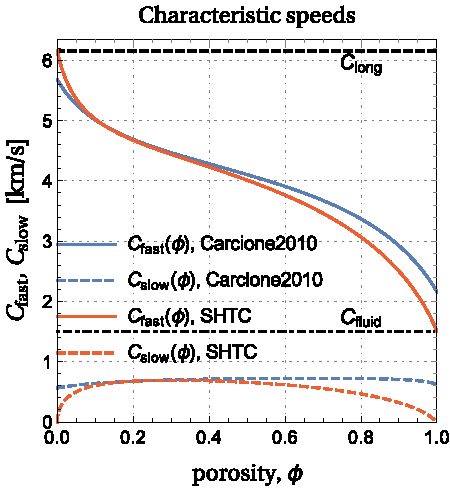
\includegraphics[draft=false,trim=0 -5 0 0,clip, 
		scale=0.75]{Figures/Characteristics}
%		&
%		\includegraphics[draft=false,trim=0 40 0 20,clip, 
%		scale=0.42]{Figures/Biot_SHTC_phi_0_2_diff_grain_modulus}
%		\end{tabular} 
		\caption{Comparison of the characteristic speeds for the Biot and SHTC 
		models for the material parameters given in 
		Table\,\ref{tab:parameters}. The Biot model is taken in the version by 
		Carcione et al \cite{Carcione2010}.  
				}  
		\label{fig:diff.grain.modulus}
	\end{center}
\end{figure}


In Fig\,\ref{fig:diff.grain.modulus}, for the two models, we compare the 
dependence of the characteristic velocities $ C_{\rm fast}(\phi) $ and $ C_{\rm 
slow}(\phi) $ of the fast 
and slow modes. Other material parameters 
are given in Table\,\ref{tab:parameters}. Remark that in order to make the 
curves closer to each other, we have had to take the bulk moduli of the solid 
phase slightly different. 

One may note that in the limit cases 
of $ \phi \to 0 $ (pure solid) and $ \phi \to 1 $ (pure fluid), the behavior of 
the characteristic speeds of the SHTC model more corresponds to what one would 
intuitively 
expects, i.e. the characteristic speeds of the mixture coincide with the 
characteristic speeds of the pure phases (horizontal dashed and dashed-dotted 
lines), while the slow mode vanishes. In 
contrast, in Biot's model the slow mode is presented even in the pure fluid or 
pure solid case. 

\begin{table}[]
	\begin{center}
		\begin{tabular}{llll}
			\hline
			Parameters\hspace{1cm}                   & Biot\hspace{2cm} & 
			SHTC          & 
			Unit                           \\ \hline
			Grain:		& & &\\[1mm]
			\rowcolor[HTML]{ECF4FF} 
			$ \rhos = \rho_2 $      & 2500   &        2500             & kg/m$ 
			^3 
			$                      \\[1mm]
			\rowcolor[HTML]{CBCEFB} 
			$ \Cs  $     &  4000       &   4332        & 
			m/s                              \\[1mm]
			\rowcolor[HTML]{ECF4FF}
			$ \Csh  $  &  -       &   3787        & 
			m/s                              \\[1mm]
			\rowcolor[HTML]{CBCEFB} 
			$ \Ks = K_2 = \rho_2 \Cs^2 $  &   40       &   46.9        & 
			GPa      \\[1mm]
			\rowcolor[HTML]{ECF4FF}
			$ \mus = \mu = \rho_2 \Csh^2 $&   -       &  35.85        & GPa 
			\\[1mm]
			%
			% 		Matrix, $\phi =0.1$		& & &\\[1mm]
			% 		\rowcolor[HTML]{CBCEFB} 
			% 		$ \Km $     & $ 15.33 $       &    -     & 
			%GPa                      \\[1mm]
			% 		\rowcolor[HTML]{ECF4FF} 
			% 		$ \mu_{\rm m} $     & $ 27.56 $       &    -     & 
			% 		GPa                      \\[1mm]
			% 		\rowcolor[HTML]{CBCEFB} 
			% 		$ \tort $     & $ 4.6 $           &   -       & 
			%-                            \\[1mm]
			% 		\rowcolor[HTML]{ECF4FF} 
			% 		$ \kappa $ & $ 2\cdot10^{-14} $      &     -     & m$ ^2 
			%$                	\\[1mm]
			% 		\rowcolor[HTML]{CBCEFB}
			% 		$ \theta_2 $       & - &  $ 9.5 \cdot10^{-7}$ & s  \\[1mm]
			%
			Matrix, $\phi =0.2$:		& & &\\[1mm]
			\rowcolor[HTML]{CBCEFB} 
			$ \Km $     & $ 9.48 $       &    -     & GPa                      
			\\[1mm]
			\rowcolor[HTML]{ECF4FF} 
			$ \mu_{\rm m} $     & $ 24.5 $       &    -     & 
			GPa                      \\[1mm]
			\rowcolor[HTML]{CBCEFB} 
			$ \tort $     & $ 3.75 $           &   -       & 
			-                            \\[1mm]
			\rowcolor[HTML]{ECF4FF} 
			$ \kappa $ & $ 1\cdot10^{-13} $      &     -     & m$ ^2 
			$                	\\[1mm]
			\rowcolor[HTML]{CBCEFB}
			$ \theta_2 $       & - &  $ 3.36\cdot10^{-7}$  & s  \\[1mm]
			%
			% 		Matrix, $\phi =0.3$		& & &\\[1mm]
			% 		\rowcolor[HTML]{CBCEFB} 
			% 		$ \Km $     & $ 6.86 $       &    -     & 
			%GPa                      \\[1mm]
			% 		\rowcolor[HTML]{ECF4FF} 
			% 		$ \mu_{\rm m} $     & $ 21.43 $       &    -     & 
			% 		GPa                      \\[1mm]
			% 		\rowcolor[HTML]{CBCEFB} 
			% 		$ \tort $     & $ 3.97 $           &   -       & 
			%-                            \\[1mm]
			% 		\rowcolor[HTML]{ECF4FF} 
			% 		$ \kappa $ & $ 1\cdot10^{-12} $      &     -     & m$ ^2 
			%$                	\\[1mm]
			% 		\rowcolor[HTML]{CBCEFB}
			% 		$ \theta_2 $       & - &  $ 1.3 \cdot10^{-5}$ & s  \\[1mm]
			%
			Fluid:		& & &\\[1mm]
			\rowcolor[HTML]{ECF4FF} 
			$ \rhof=\rho_1 $ & 1040        &     1040       & kg/m$ ^3 
			$              \\[1mm]
			\rowcolor[HTML]{CBCEFB} 
			$ \Cf $ & 1500        &     1500       & 
			m/s                              \\[1mm]
			\rowcolor[HTML]{ECF4FF} 
			$ \Kf =K_1=\rhof \Cf^2$     & 2.34          &   2.34       & 
			GPa                   
			\\[1mm]
			\rowcolor[HTML]{CBCEFB} 
			$ \eta $  & $ 10^{-3} $&    -      & Pa$ \cdot $ s             
			\\[1mm]
			\hline
		\end{tabular}
		\caption{ Material parameters for the Biot and SHTC model. Here, 
		$C_{\rm s}$ and $C_{\rm f}$ are the bulk sound speeds in the solid and 
		fluid accordingly.}
		\label{tab:parameters}
	\end{center}
\end{table}


\subsubsection{Dispersion relations and sound speeds}


In this section, we perform the plain wave analysis of the SHTC and Biot 
models. Moreover, we shall 
consider only longitudinal waves. In this case the vector of SHTC state 
variables reduces to 
\begin{equation}
\QQ = (v_1,w_1,p,s_{11}).
\end{equation}
After linearizing the right hand-side of system \eqref{eqn.1Dfull} in a 
neighborhood of $ \QQ = \QQ_0 + \qq $, where $ \qq 
$ is a small perturbation of the equilibrium state $ \QQ_0 = (0,0,p_0,0) $, one obtains
\begin{equation}\label{eqn.perturb}
\qq_t + \mathbb{A}\qq_x = \mathbb{S}\qq,
\end{equation}
where the matrices $ \mathbb{A} $ and $ \mathbb{S} = \pd\SS/\pd\QQ $ are taken 
at the equilibrium state $ \QQ_0 $ and read as
\begin{equation}\label{eqn.1d.matrices}
\mathbb{A} = \left( \begin{array}{cccc}
0 & 0 & \rho^{-1} & \alpha_{2}\rho^{-1} \\ 
0 & 0 & R & 0 \\ 
K & K' & 0 & 0 \\ 
-\frac43\mu & 0 & 0 & 0
\end{array} \right), \qquad
\mathbb{S} = \left( \begin{array}{cccc}
0 & 0 & 0 & 0 \\ 
0 & -\frac{1}{\theta_2'} & 0 & 0 \\ 
0 & 0 & 0 & 0 \\ 
0 & 0 & 0 & 0
\end{array} \right).
\end{equation}

We then look for the solution that have the form
\begin{equation}\label{eqn.qq}
\qq = \tilde{\qq} e^{\text{i}(\omega t - k x)}
\end{equation}
representing a plane harmonic wave of real frequency $ \omega $ and complex wave number $ k $ 
propagating in the direction $ x $, and $ \tilde{\qq} = const $ is the constant 
vector of amplitudes. 
By substituting \eqref{eqn.qq} in \eqref{eqn.perturb}, one obtains the homogeneous linear system on 
$ \tilde{\qq} $ \cite{Ruggeri1992,Ruggeri2015}
\begin{equation}\label{eqn.lin.dispers}
\left(\mathbb{I} - \frac{k}{\omega} \mathbb{A} + \frac{\text{i}}{\omega} \mathbb{S} \right) 
\tilde{\qq} = 0
\end{equation}
where $ \mathbb{I} $ is the identity matrix of the same size as $ \mathbb{A} $ 
and $ \mathbb{S} $. From \eqref{eqn.lin.dispers}, one obtains the dispersion relation for 
\eqref{eqn.1Dfull}
\begin{equation}\label{eqn.dispers.rel}
\det\left(\mathbb{I} - \frac{k}{\omega} \mathbb{A} + \frac{\text{i}}{\omega} \mathbb{S} \right) = 0.
\end{equation}
The phase velocity $ V_{\rm ph} $ (sound speed) and the attenuation factor $ a 
$ are then given by
\begin{equation}
V_{\rm ph} = \frac{\omega}{{\rm Re}(k)}, \qquad a = -{\rm Im}(k).
\end{equation}
In addition, it is convenient to use the attenuation per wavelength 
\cite{Ruggeri2015}
\begin{equation}\label{atten.wavelength}
a_\lambda = a \lambda = \frac{2 \pi V_{\rm ph} a }{\omega} = -2 \pi \frac{{\rm 
Im}(k)}{{\rm Re}(k)},
\end{equation}
where $ \lambda $ is the wavelength.

One can find that the four solutions to \eqref{eqn.dispers.rel} with matrices 
\eqref{eqn.1d.matrices} are 
	\begin{equation}
	k(\omega) = \pm \omega \sqrt{\frac{X+Y - {\rm i}(Y+Z)/\Omega\pm \sqrt{4 Y 
	(X-Z)({\rm i}/\Omega-1) + 
	({\rm i}(Y+Z)/\Omega - (X + Y))^2}}{2(X-Z)Y}},
	\end{equation}
where $ X, Y $, and $ Z $ are defined in \eqref{speeds.SHTC}, and $ \Omega = 
\omega \theta_2' $ is the non-dimensional frequency.

Performing the same analysis for the Biot equations \eqref{eqn.Biot.model}, one 
obtains that the dispersion relation is a bi-quadratic equation 
\begin{subequations}
	\begin{equation}\label{Biot.disp}
		\lambda^4 + a_2 \lambda^2 + a_0 = 0,
	\end{equation}
	\begin{equation}\label{a2.Biot}
		a_2 = \omega  \left(-\frac{\omega  (\tort \rhof 
		(\lambdau +2 \muu )+M \phi  (\rho -2 \alpha  \rhof))}{\phi 
		M \left(\lambdau +2 \muu - \alpha ^2 M\right)}+\frac{{\rm i} \eta  
		(\lambdau +2 \muu )}{\kappa M \left(\lambdau +2 \muu - \alpha ^2 
		M\right)}\right),
	\end{equation}
	\begin{equation}\label{a0.Biot}
		a_0 = \omega ^3 \left(\frac{\rhof \omega  (\tort \rho -\rhof \phi 
		)}{\phi M  \left(\lambdau +2 \muu - \alpha ^2 M\right)}-\frac{{\rm i} 
		\eta  
		\rho }{\kappa M \left(\lambdau +2 \muu - \alpha ^2 M\right)}\right).
	\end{equation}
\end{subequations}

Finally, we plot the phase velocities $ V_{\rm ph}(\omega) $ and attenuation 
factor per wavelength $ a_{\lambda}(\omega) $ of the fast and slow sound waves 
for the both models in Fig.\,\ref{fig:Vph.Attenuation}. One 
may note the difference in the high-frequency limit of the fast modes 
which is, in fact, due to the 
difference in the characteristic speeds $ C_{\rm fast} $ and $ C_{\rm slow} $ 
depicted in 
Fig.\,\ref{fig:diff.grain.modulus}. Indeed, recall that the characteristic 
speeds (the eigenvalues of the homogeneous hyperbolic system) are the 
high-frequency limits ($ \omega \to \infty $) of the sound speeds (the 
eigenvalues of the non-homogeneous system \eqref{eqn.perturb}) 
\cite{Ruggeri1992,Ruggeri2015,DPRZ2016}.
The slow mode dispersion curves of the both models are almost 
indistinguishable, see 
Fig.\,\ref{fig:Vph.Attenuation}, second column.

Another conclusion is the big difference ($ \sim 10^3 $) in the attenuation 
factor $ a_\lambda $ of the fast and slow modes for the both models in the low 
frequency region, see Fig.\,\ref{fig:Vph.Attenuation}, second row.

\begin{figure}[!htbp]
	\begin{center}
			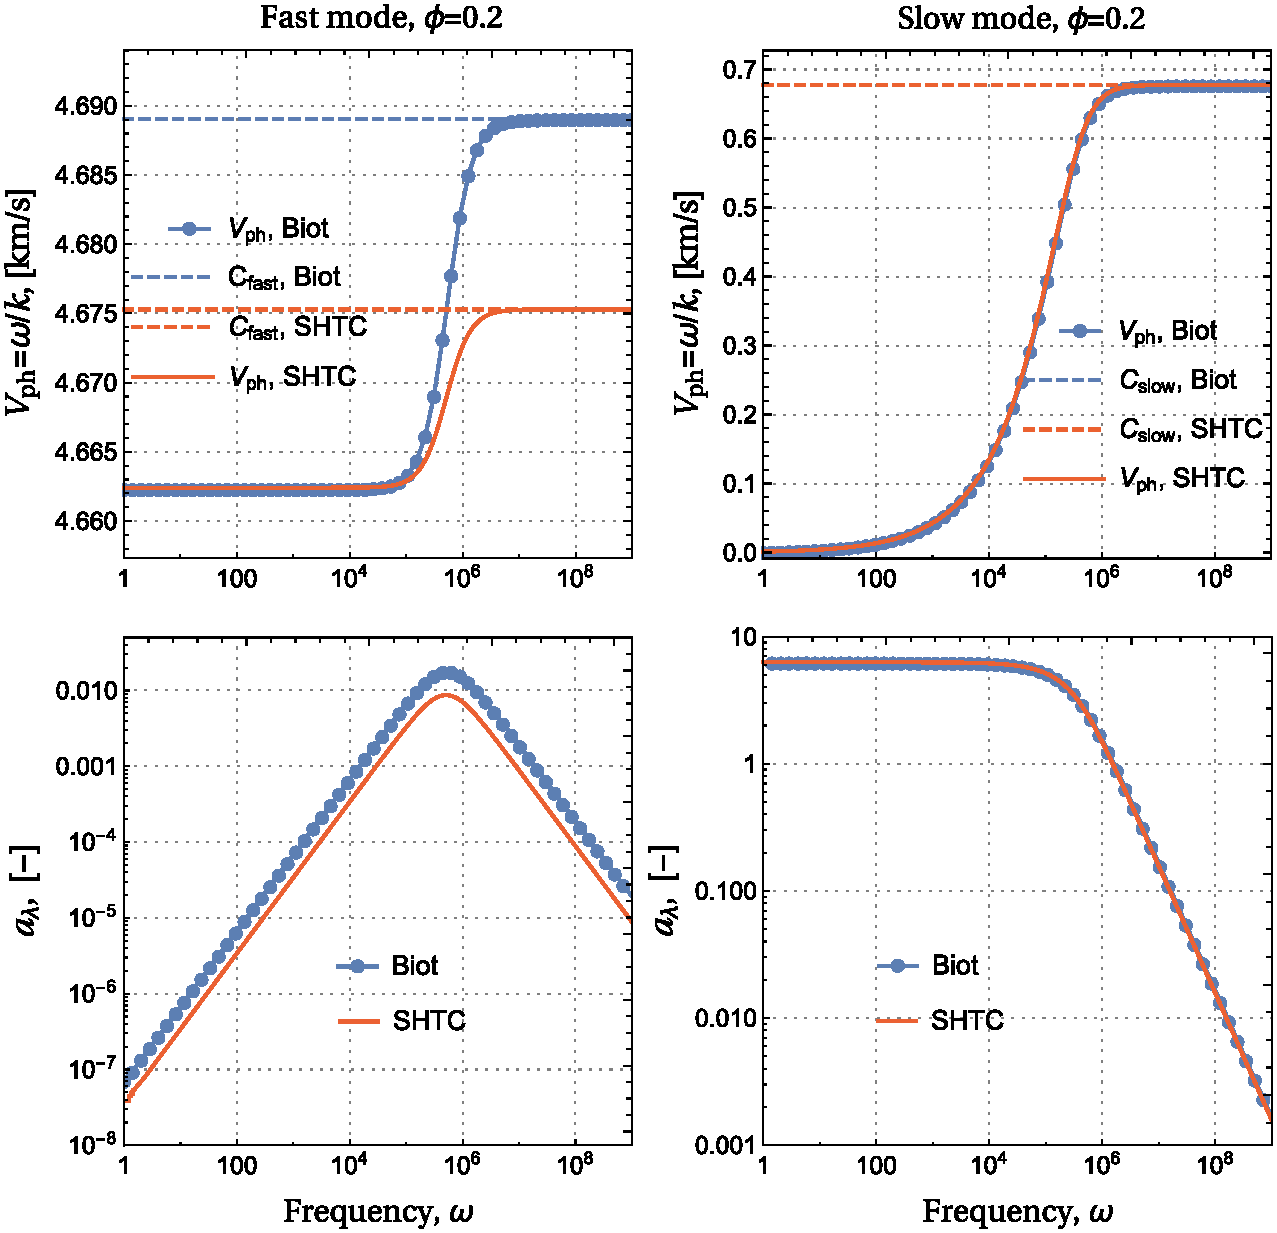
\includegraphics[draft=false,trim=0 0 0 0,clip, 
			scale=0.42]{Figures/Vph-AttenuationLog}
		\caption{Phase velocities (first row) and attenuation factors per 
			wavelength (second row) for the fast (first column) and slow 
			(second column) modes of the SHTC and Biot models. The material 
			parameters are given in Table\,\ref{tab:parameters}.  
		}  
		\label{fig:Vph.Attenuation}
	\end{center}
\end{figure}



%\begin{figure}
%	\begin{center}
%		
%\includegraphics[draft=false,width=0.70\textwidth]{Figures/Biot_SHTC_diff_grain_phi_0_2_symb}
%	\end{center}
%	\vspace{-8mm}
%	\caption{{\footnotesize \it {\color{red}Porosity, $\phi=0.2$:}Comparison of the phase 
%velocities $V_{\rm ph}=\omega/k$  for the 
%	SHTC 
%	(red curves) and Biot (blue curves) models for the parameters from Table\,\ref{tab.parameters}: 
%	fast pressure waves (a) and slow pressure waves 
%	(b). The dashed blue  and red lines are the characteristic speeds for the Biot model and SHTC 
%	model.}}
%	\label{fig.dispersion}
%\end{figure}


\section{Numerical test problems for small amplitude wave 
propagation}\label{sec.numerics}

\subsection{Finite difference implementation}
To discretize the governing equations, the velocity-stress formulation, 
proposed for elastic-wave equations  \cite{Levander1988,Virieux1986} is used. 
The choice of the numerical scheme on staggered grids looks very natural due to 
the fact that equations form the symmetric first order system of evolution 
equations for the components of mixture and relative velocities, pressure and 
shear stress.

Following the notations from \cite{Virieux1986} and \cite{Graves1996}, we 
introduce the time-space grid with integer nodes $t^{n}=n\Delta t$, 
$x_{i}=i\Delta 
x$, $y_{j}=j\Delta y$  and half-integer nodes $t^{n+1/2}=(n+1/2)\Delta t$, 
$x_{i+1/2}=(i+1/2)\Delta x$, $y_{j+1/2}=(j+1/2)\Delta y$ , where  $\Delta t$, 
$\Delta x$ and $\Delta y$ denote the grid steps along the temporal and spatial 
coordinates.

 For a discrete function $f_{i,j}^{n}=f(t^{n},x_{i},y_{j})$ defined in the grid 
 nodes,  let us introduce the second-order  centered finite-difference 
 operators:
\begin{equation}
    D_t[f]_{i, j}^{n} = \frac{(f)_{i, j}^{n+1/2} - (f)_{i, j}^{n-1/2}}{\Delta t}, \qquad A_t[f]_{i, j}^{n} = \frac{(f)_{i, j}^{n+1/2} + (f)_{i ,j}^{n-1/2}}{2},
    \label{Dt}
\end{equation}
\begin{equation}
    D_x[f]_{i, j}^n = \frac{(f)_{i+1/2, j}^{n} - (f)_{i-1/2, j}^{n}}{\Delta x}, \qquad D_y[f]_{i, j}^n = \frac{(f)_{i, j+1/2}^{n} - (f)_{i, j-1/2}^{n}}{\Delta y}.
    \label{Dx}
\end{equation}

The material parameters are constant within each grid cell 
$[x_{i-1/2}, x_{i+1/2}] \times[ y_{j-1/2}, y_{j+1/2}]$ and allowed to have 
discontinuities aligned with the grid lines. This condition provides the 
second-order of convergence even for discontinuous material parameters 
\cite{Moszo2002}.

The wavefield components are defined at different time-space grid nodes. The 
components of the mixture and relative velocities are defined as $(v_x)_{i+1/2, 
j}^{n}$, $(v_y)_{i, j+1/2}^{n}$, $(w_x)_{i+1/2, j}^{n}$, $(w_y)_{i, 
j+1/2}^{n}$, the pressure and normal components of the deviatoric stress as 
$(p)_{i,j}^{n+1/2}$,  $(s_{xx})_{i,j}^{n+1/2}$, $(s_{yy})_{i,j}^{n+1/2}$, and 
the shear stress as $(s_{xy})_{i+1/2, j+1/2}^{n+1/2}$.

To construct the finite difference scheme, we apply the finite volume 
approximation  or balance law technique \cite{Samarskii2001}. Thus, the 
discrete form 
of equations \eqref{stress.velocity} reads
\begin{subequations}
\begin{equation}\label{eq:v1}
\begin{array}{c}
D_t[v_x]_{i+1/2 ,j}^{n-1/2} =- \left \langle 1/\rho^{0} \right \rangle_{i+1/2,j}D_x[P]_{i+1/2 ,j}^{n-1/2} +\\
+ \left \langle\alpha_{2}^{0}/ \rho^{0} \right \rangle_{i+1/2,j} \left( D_x[s_{xx}]_{i+1/2, j}^{n-1/2} + D_y[s_{xy}]_{i+1/2, j}^{n-1/2} \right), 
\end{array}
\end{equation}
\begin{equation}\label{eq:v2}
\begin{array}{c}
D_t[v_y]_{i ,j+1/2}^{n-1/2} =- \left \langle 1/\rho^{0} \right \rangle_{i,j+1/2}D_y[P]_{i ,j+1/2}^{n-1/2} +\\
+ \left \langle\alpha_{2}^{0}/ \rho^{0} \right \rangle_{i,j+1/2} \left( D_x[s_{xy}]_{i, j+1/2}^{n-1/2} + D_y[s_{yy}]_{i, j+1/2}^{n-1/2} \right), 
\end{array}
\end{equation}
\begin{equation}\label{eq:w1}
\begin{array}{c}
D_t[w_x]_{i+1/2 ,j}^{n-1/2} =- \left \langle 1/\rho_{1}^{0}-1/\rho_{2}^{0} \right \rangle_{i+1/2,j}D_x[P]_{i+1/2 ,j}^{n-1/2} - \\
- \left \langle c_{1}^{0}c_{2}^{0}/\theta_{2} \right \rangle_{i+1/2,j}A_t[w_x]_{i+1/2 ,j}^{n-1/2} ,
\end{array}
\end{equation}
\begin{equation}\label{eq:w2}
\begin{array}{c}
D_t[w_y]_{i ,j+1/2}^{n-1/2} =- \left \langle 1/\rho_{1}^{0}-1/\rho_{2}^{0} \right \rangle_{i,j+1/2}D_y[P]_{i ,j+1/2}^{n-1/2} - \\
- \left \langle c_{1}^{0}c_{2}^{0}/\theta_{2} \right \rangle_{i,j+1/2}A_t[w_y]_{i ,j+1/2}^{n-1/2} ,
\end{array}
\end{equation}
\begin{equation}\label{eq:s11}
D_t[s_{xx}]_{i ,j}^{n} = (\mu)_{i ,j} \left (\frac{4}{3} D_x[v_x]_{i ,j}^{n} - \frac{2}{3} D_y[v_y]_{i ,j}^{n}\right ) -  (\alpha_{2}^{0}/\tau)_{i,j} A_t[s_{xx}]_{i,j}^{n},
\end{equation}
\begin{equation}\label{eq:s22}
D_t[s_{yy}]_{i ,j}^{n} = (\mu)_{i ,j} \left (\frac{4}{3} D_y[v_y]_{i ,j}^{n} - \frac{2}{3} D_x[v_x]_{i ,j}^{n}\right ) - (\alpha_{2}^{0}/\tau)_{i,j}  A_t[s_{yy}]_{i,j}^{n},
\end{equation}
\begin{equation}\label{eq:s12}
\begin{array}{c}
D_t[s_{xy}]_{i+1/2 ,j+1/2}^{n} = \left \{ \mu \right \}_{i+1/2 ,j+1/2} \left ( D_x[v_y]_{i+1/2 ,j+1/2}^{n} + D_y[v_x]_{i+1/2 ,j+1/2}^{n}\right ) -\\
-  \left \{ \alpha_{2}^{0}/\tau  \right \}_{i+1/2 ,j+1/2} A_t[s_{xy}]_{i+1/2 ,j+1/2}^{n},
\end{array}
\end{equation}
\begin{equation}\label{eq:p}
\begin{array}{c}
D_t[P]_{i ,j}^{n}  = -  (K)_{i ,j}  \left (D_x[v_x]_{i ,j}^{n} +D_y[v_y]_{i ,j}^{n}\right ) - \\
-\left ( (\rho_{2}^{0}-\rho_{1}^{0})\alpha_{1}^{0}\alpha_{2}^{0}K/\rho^{0}\right )_{i ,j}\left (   D_x[w_x]_{i ,j}^{n} +  D_y[w_y]_{i ,j}^{n} \right ),
\end{array}
\end{equation}
\end{subequations}
where the effective medium parameters on the staggered grids are obtained as 
the volume arithmetic or harmonic averaging \cite{Moszo2002}:
\begin{equation}\label{eq:notations}
\begin{array}{c}
\left \langle f\right \rangle_{i+1/2,j}=(f_{i,j}+f_{i+1,j})/2, \qquad 
\left \langle f\right \rangle_{i,j+1/2}=(f_{i,j}+f_{i,j+1})/2,\\[2mm]
\left \{ f \right \}_{i+1/2 ,j+1/2}  =\left \lfloor   \left(   1/f_{i,j}+1/f_{i+1,j}+1/f_{i,j+1}+1/f_{i+1,j+1}\right) /4\right \rfloor ^{-1}.
\end{array}
\end{equation}

The obtained 2D velocity-stress finite difference scheme is second-order in 
time and space.  Note that the approximation can be easily improved by using 
higher order operators.  The well-known Courant-Friedrich-Lax (CFL) stability 
criterion also holds for this case. Thus, the time step must be 
chosen small enough in order the fastest characteristic wave (P-wave) 
$C_{max}$ 
travels the distance smaller than the spatial discretization step:
$$
\Delta t C_{max}\sqrt{\frac{1}{{\Delta x}^{2}}+\frac{1}{{\Delta y}^{2}}}\leq 1.
$$

A forcing function $f(t,x,y)$ is introduced as the source term on the right 
hand side of the pressure equation or the equations for the normal components 
of 
the deviatoric stress in system \eqref{stress.velocity}. In both cases, a 
volumetric-type source term is obtained. Furthermore, the source function is 
defined as the product of Dirac's delta in space and Ricker's wavelet in time 
\begin{equation}
f(t)=(1-2\pi ^{2} f_{0}^{2}(t-t_{0})^{2})exp[-\pi ^{2}f_{0}^{2}(t-t_{0})^{2}],
\end{equation}
where $f_{0}$ is the source peak frequency and $t_{0}$ is the wavelet delay.

No special care is applied to suppress outgoing waves with the help of absorbing boundary conditions (for example, PML). The simulation is stopped before the waves have reached the boundaries of the computational domain. 
The numerical experiments were conducted on a desktop computer Intel(R) 
Core(TM) i7 3.60 GHz processor.

In the subsequent sections, we illustrate the main features of the 
wavefield formation and propagation depending on the porosity $\phi$, 
friction parameter $\theta_2$, source peak frequency $f_{0}$ and  shear relaxation time $\tau$. Before doing 
this, we start with considering the homogeneous (dissipation-less) case.

\subsection{Dependence on the porosity $\phi$.}

The computational domain $\Omega =[-0.65, 0.65]^{2}$  m was discretized with 
$ N_x \times N_y$ grid points, $N_x = N_y = 3250$, which amounts to 10 points 
per 
slow 
compressional wavelength in $\Omega$ for a source of central frequency 
$f_0=10^{5} $ Hz  and for various values of the porosity $\phi$. The model 
parameters were taken from Table\,\ref{tab:parameters}. The source was located 
in the center of the computational 
domain. Propagation time was chosen equal to $T_{0}= 1.1\cdot10^{-4}$ s  with 
taking into account the source time delay $t_{0}=1/f_{0}$=$ 0.1\cdot10^{-4}$ s. 
The time step was chosen according to 
the classical Courant stability criterion for staggered grids with $CFL = 0.9$. 


Fig.\,\ref{fig:porosity 0}(a) shows a snapshot of the mixture velocity $v^1$  
at time $T_{0}$, on the whole computational domain. The porosity parameter was 
chosen equal to $\phi$=0, that corresponds to the case of a pure elastic solid. 
In an elastic medium, only one fast P-wave with the velocity  equal to 6155 m/s 
is 
excited from a source of volumetric type. The seismogram on Fig.\,
\ref{fig:porosity 0}(b) confirms the occurrence of this wave with predicted 
velocity. The receivers were located along the $ x $-direction starting from 
the source point towards the boundary with a uniform 
spacing between the receivers.
\begin{figure}[!htbp]
\begin{subfigure}{0.5\linewidth}
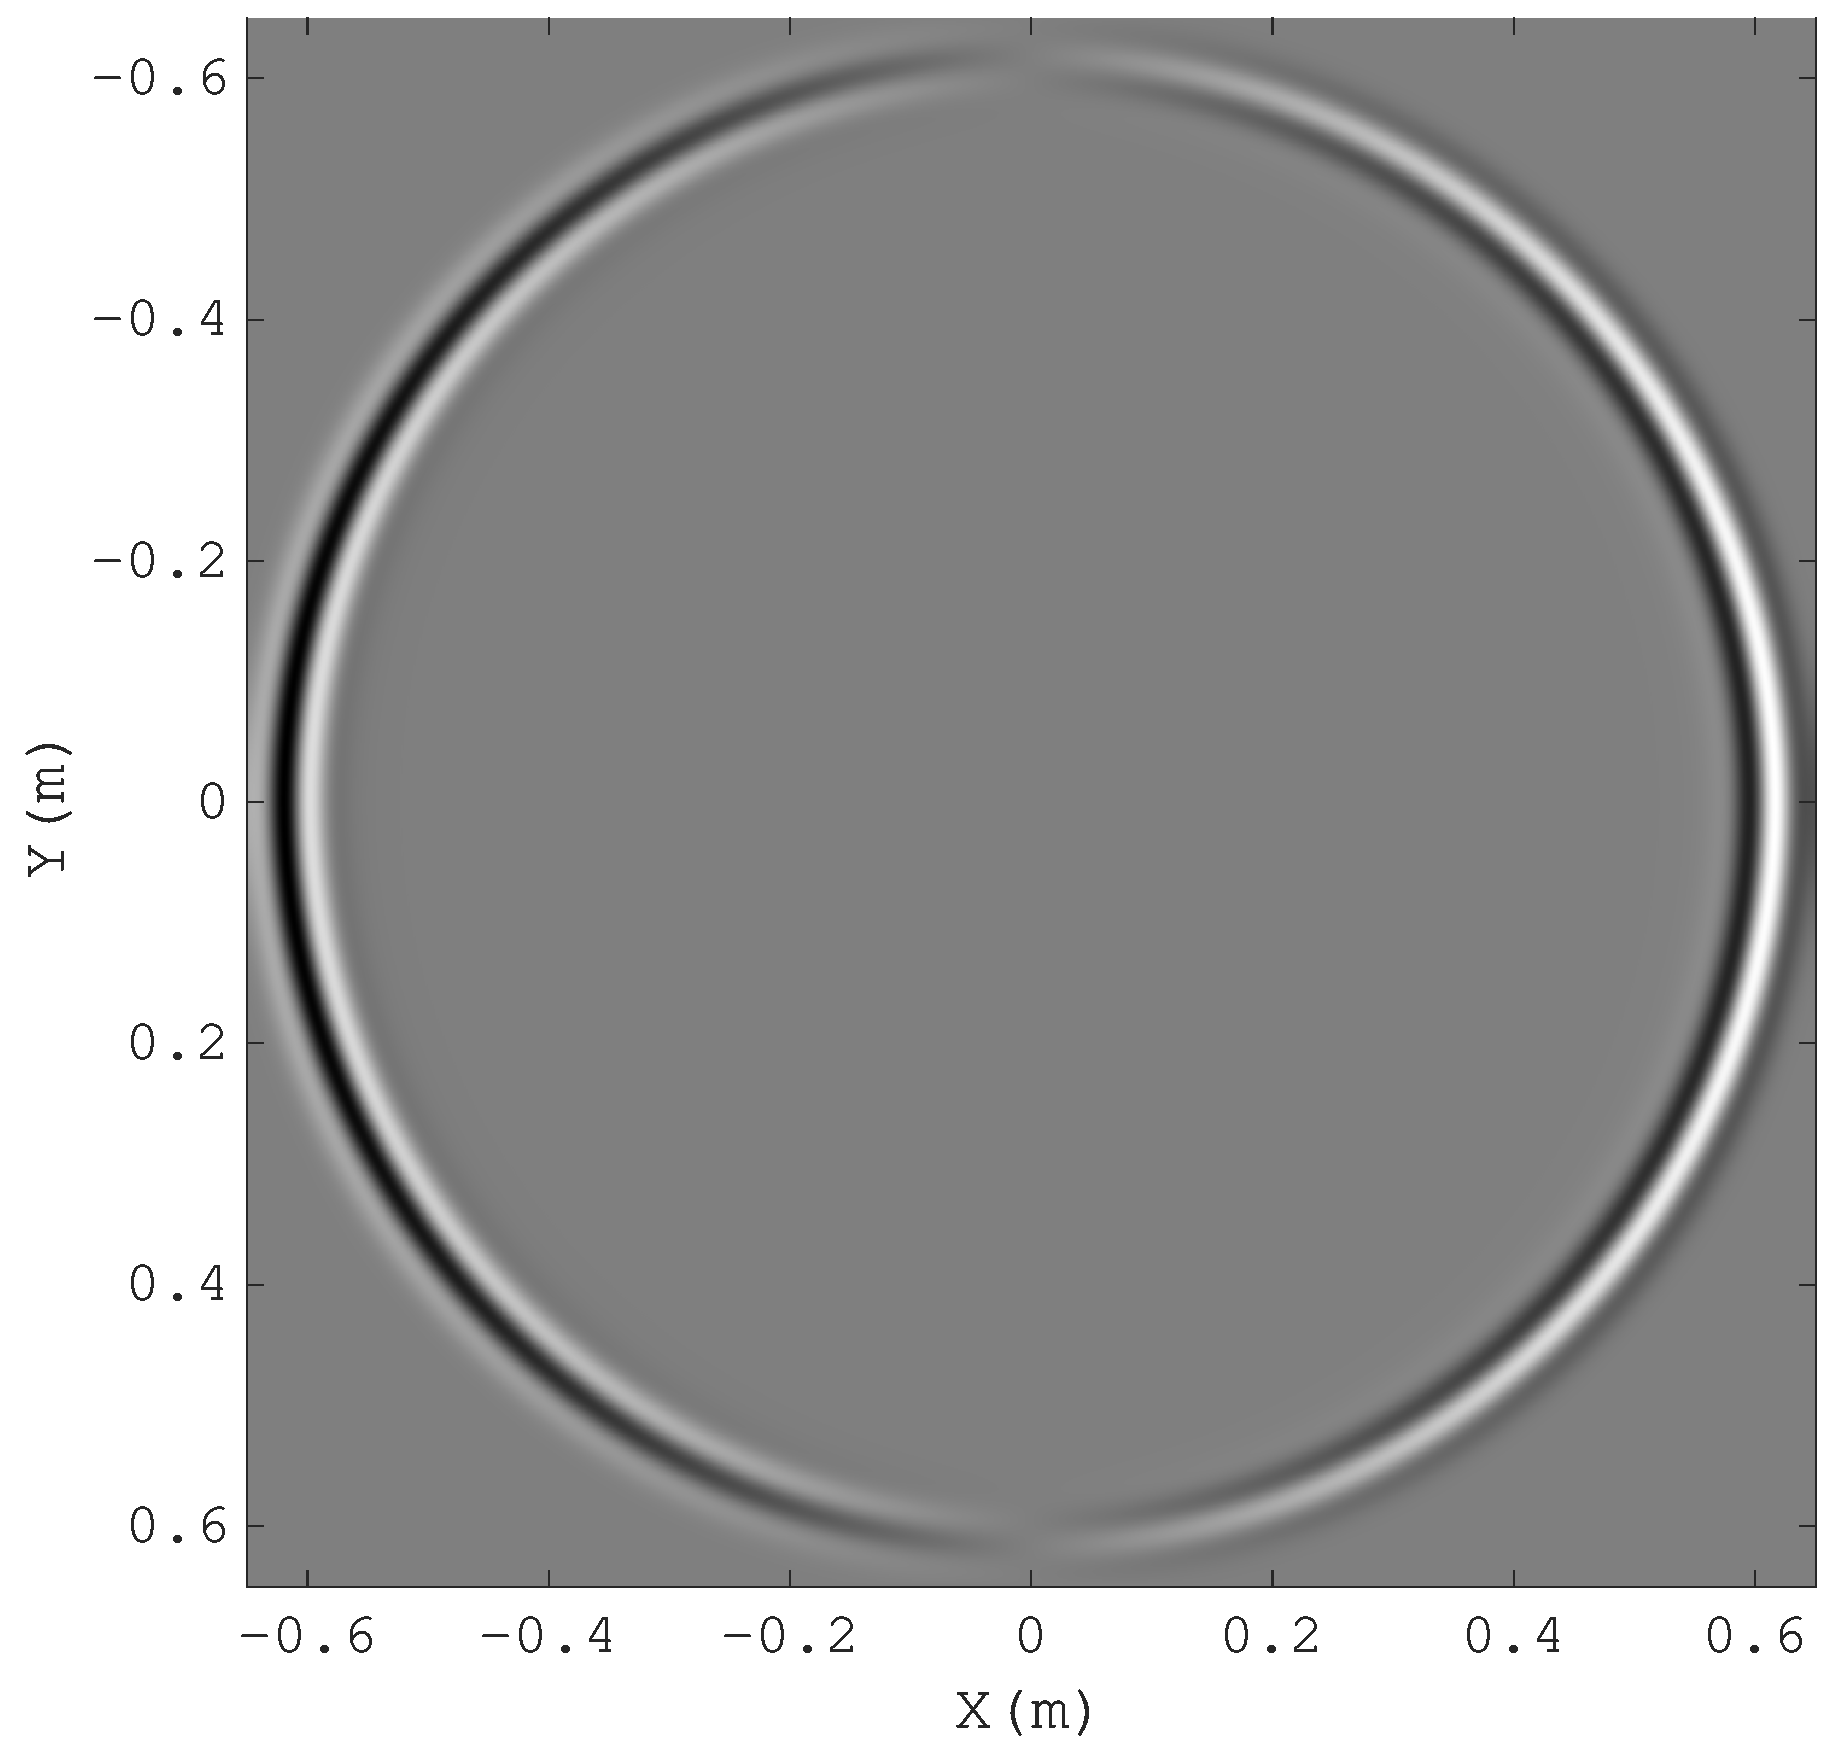
\includegraphics[draft=false,width=0.7\textwidth]{Figures/wave_alfa_s_1}
\caption{}
\end{subfigure}
\hfill
\begin{subfigure}{0.5\linewidth}
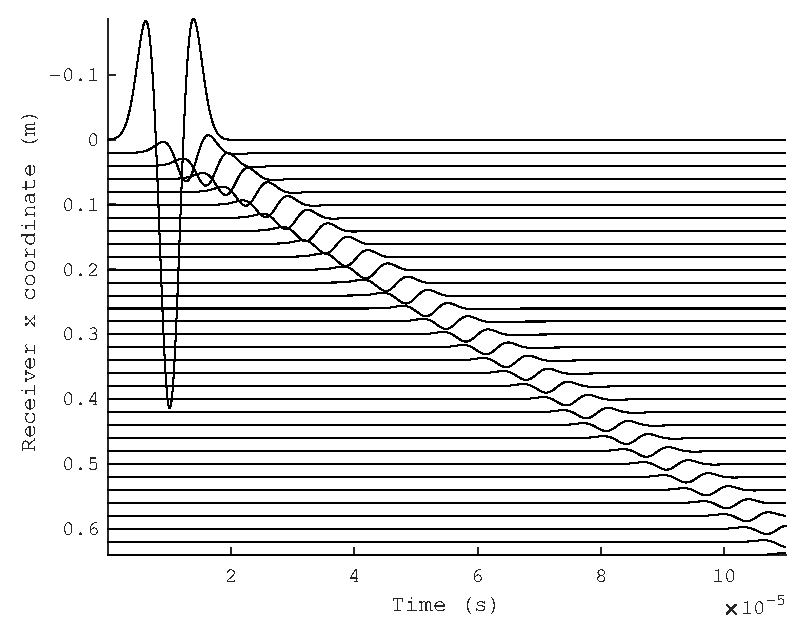
\includegraphics[draft=false,width=0.8\textwidth]{Figures/alfa_s_1}
\caption{}
\end{subfigure}%
\caption{A snapshot at time $T_{0}$ (a) and seismogram (b) of the mixture 
velocity $v^1$  for source of central frequency $f_{0} =10^{5} $ Hz and 
porosity 
parameter $\phi$=0.}
\label{fig:porosity 0}
\end{figure}

The Fig.\,\ref{fig:porosity 1} shows calculations similar to the previous one 
but with the porosity parameter $\phi$=1. This corresponds to the case of pure 
liquid with one pressure wave with the velocity 1500 m/s. The numerical 
propagation velocity can be easily estimated from the computed seismogram in  
Fig.\,\ref{fig:porosity 1}(b) and equal exactly 1500 m/s.
\begin{figure}[!htbp]
\begin{subfigure}{0.5\linewidth}
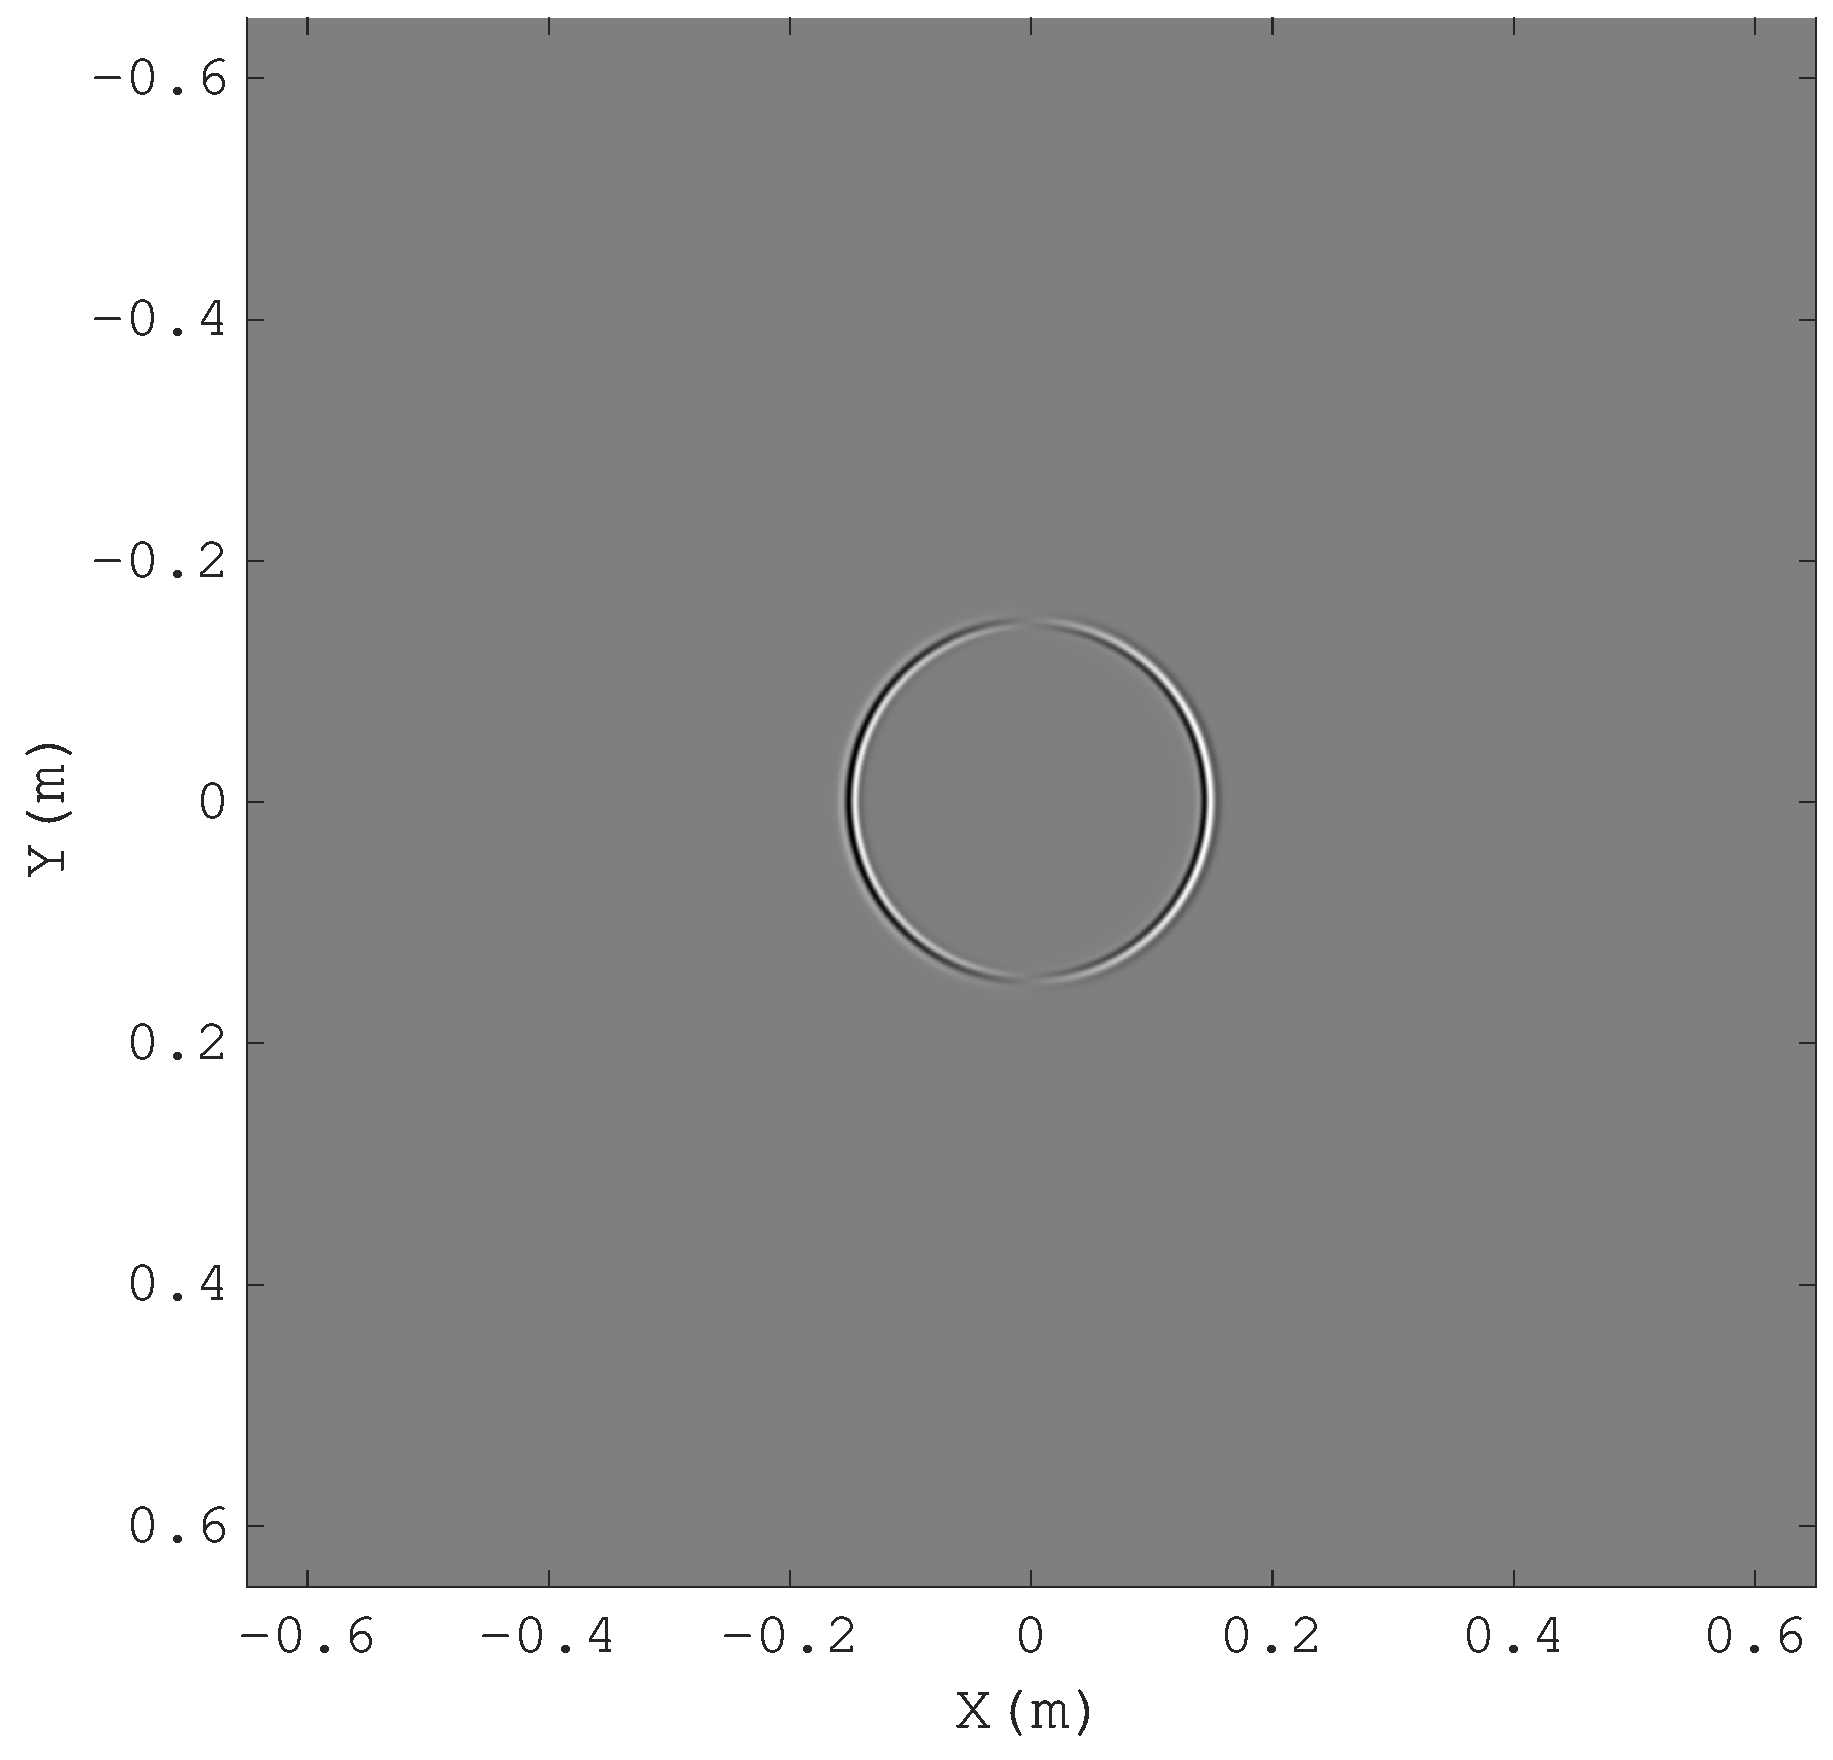
\includegraphics[draft=false,width=0.7\textwidth]{Figures/wave_alfa_s_00}
\caption{}
\end{subfigure}
\hfill
\begin{subfigure}{0.5\linewidth}
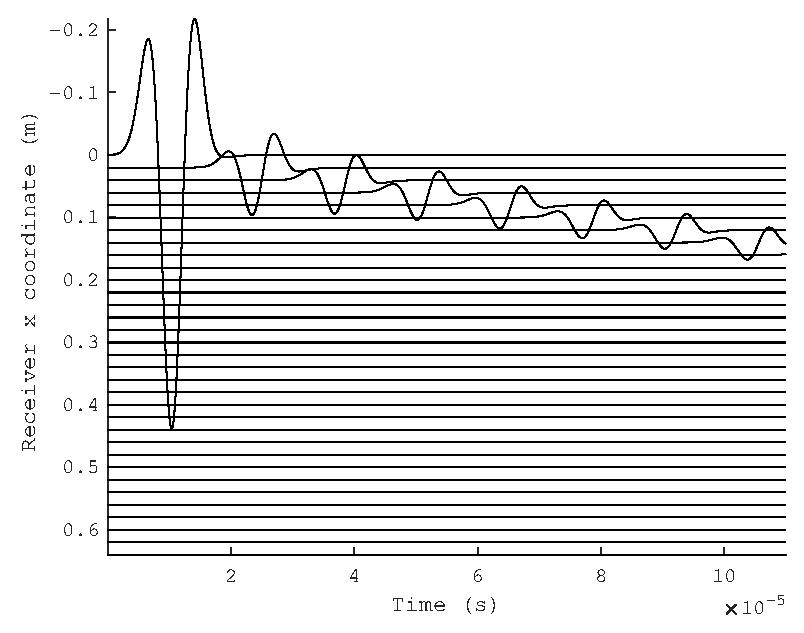
\includegraphics[draft=false,width=0.8\textwidth]{Figures/alfa_s_00}
\caption{}
\end{subfigure}%
\caption{A snapshot at time $T_{0}$ (a) and seismogram (b) of the mixture 
velocity $v^1$  for source of central frequency $f_{0} =10^{5} $ Hz  and 
porosity 
parameter $\phi$=1.}
\label{fig:porosity 1}
\end{figure}

The simulation for the porosity parameter $\phi$=0.5 is shown in 
Fig.\,\ref{fig:porosity 05}. The fast P-wave velocity is estimated at 4100 m/s 
from the
computed seismogram in  Fig.\,\ref{fig:porosity 05}(b) and is consistent with 
the data from Table\,\ref{tab:parameters}. In snap Fig.\,\ref{fig:porosity 
05}(a) we do not observe the predicted slow P-wave because its amplitude is 
very 
small, completely attenuates and is not visible at this time moment. However, 
if we 
zoom in the image, we will be able to see this slow P-wave in 
Fig.\,\ref{fig:porosity 05 zoom}.
\begin{figure}[!htbp]
\begin{subfigure}{0.5\linewidth}
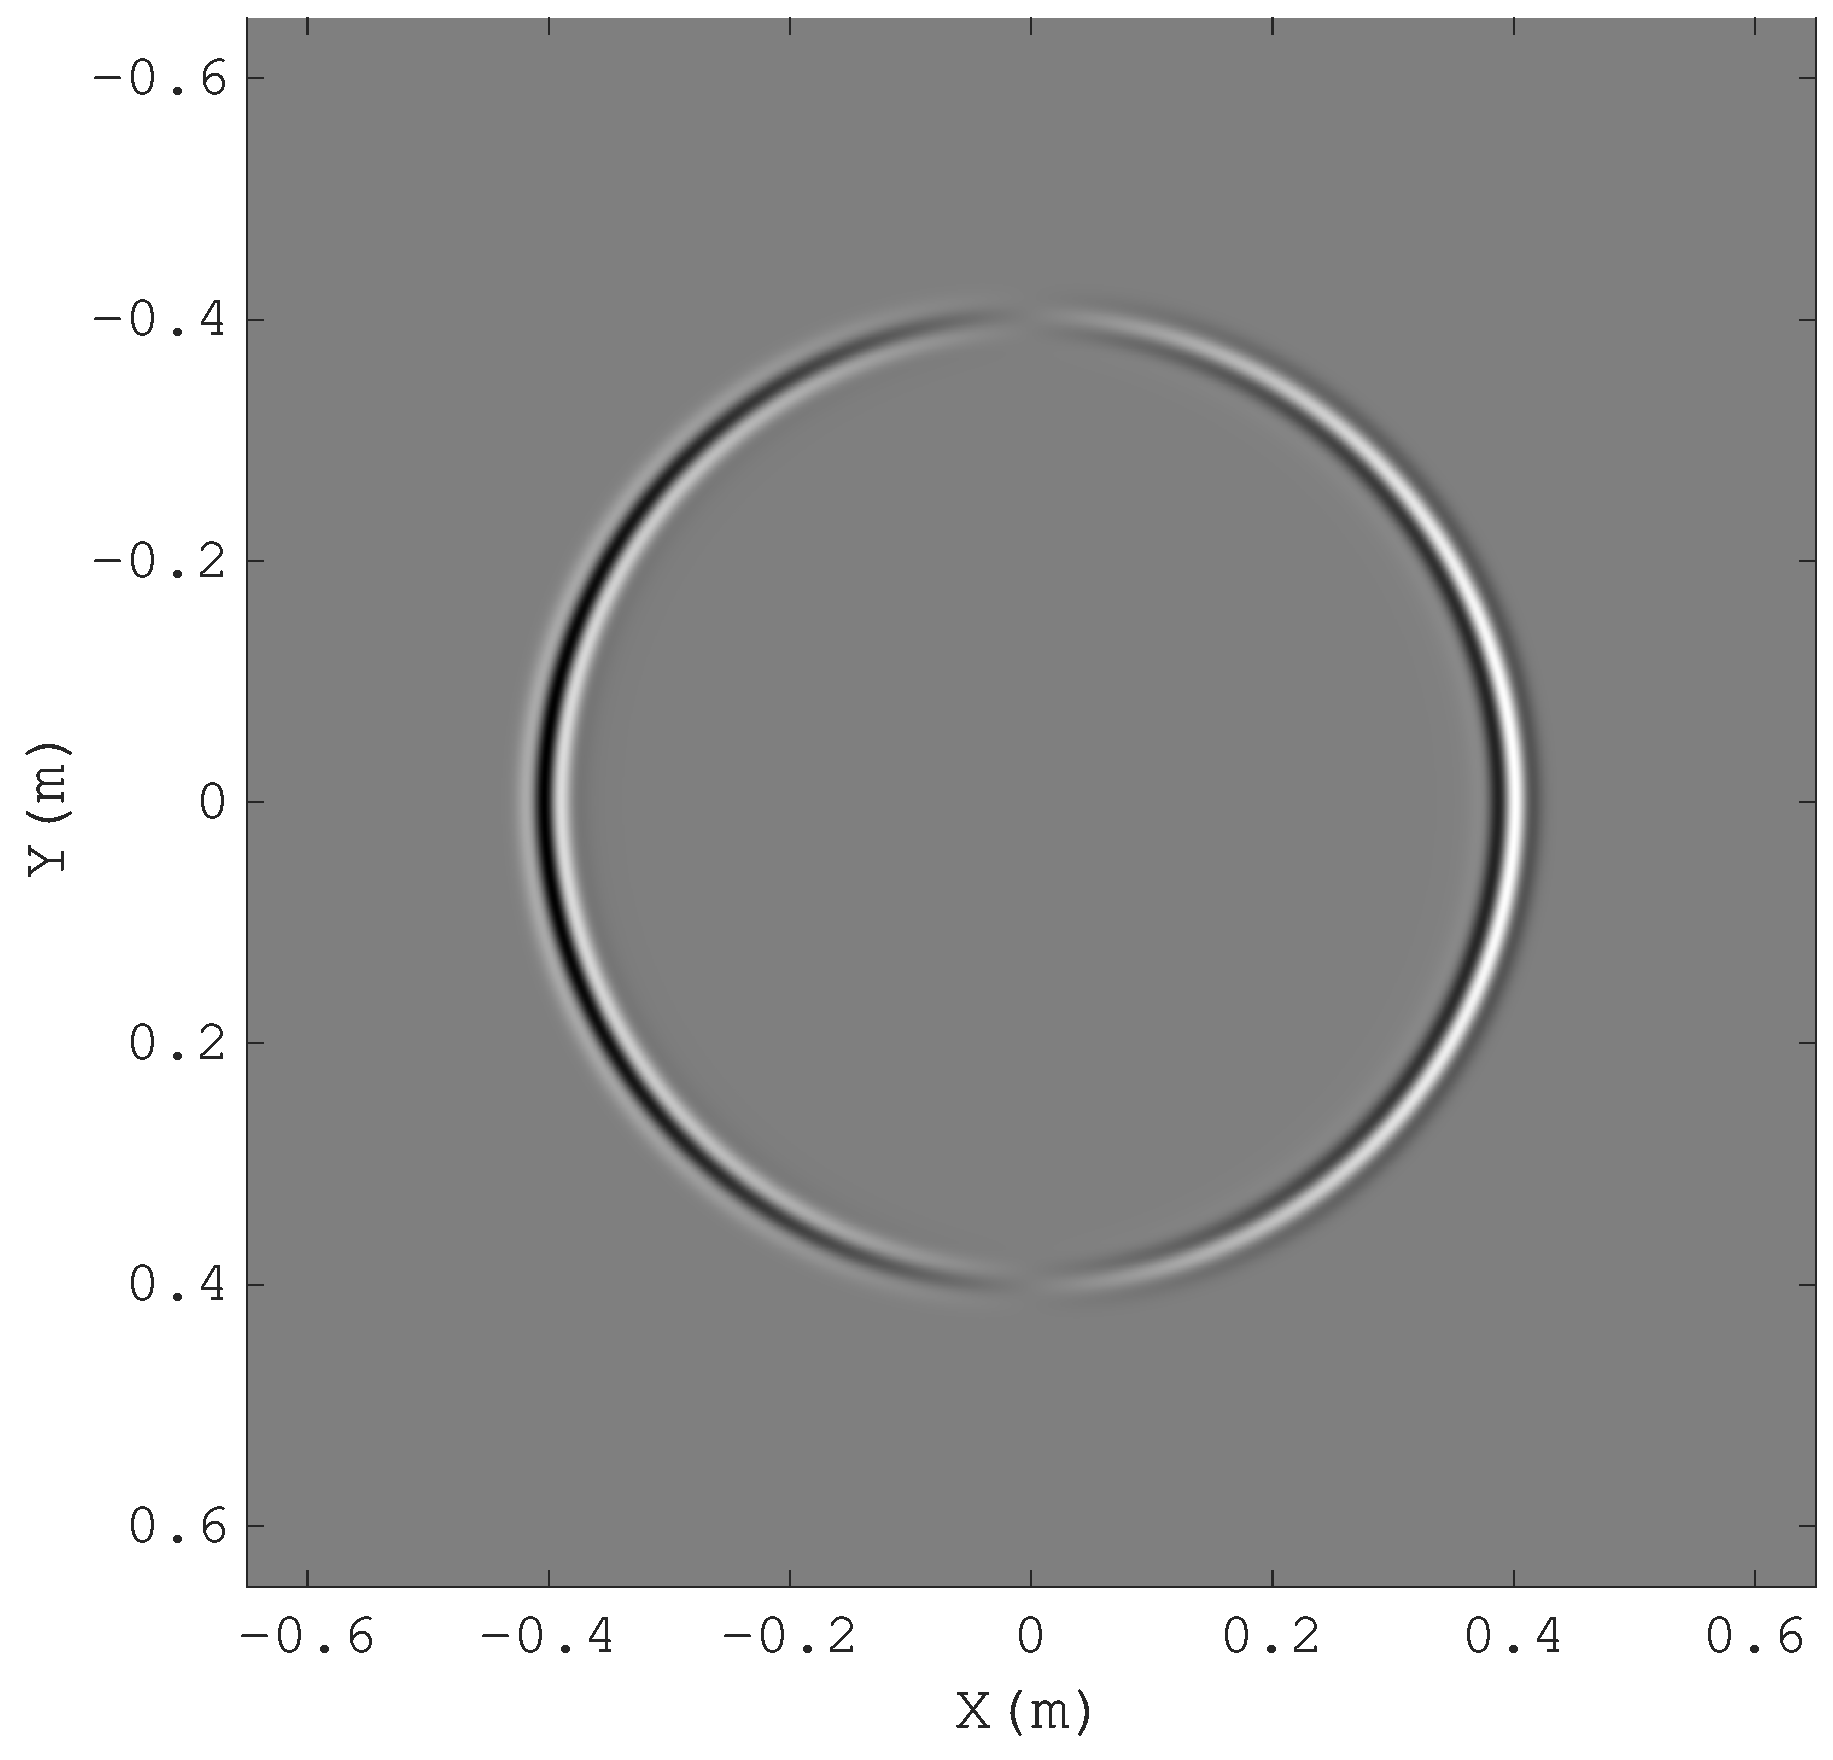
\includegraphics[draft=false,width=0.7\textwidth]{Figures/wave_alfa_s_05}
\caption{}
\end{subfigure}
\hfill
\begin{subfigure}{0.5\linewidth}
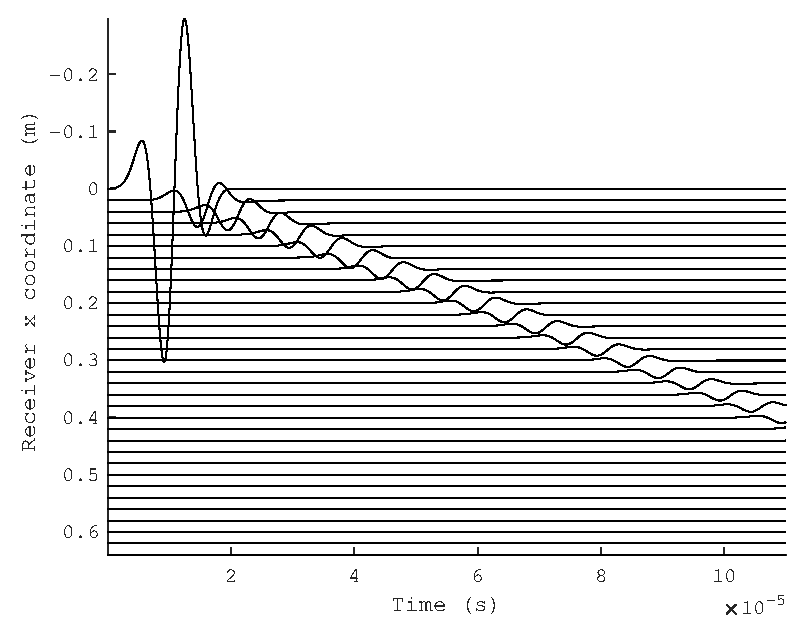
\includegraphics[draft=false,width=0.8\textwidth]{Figures/alfa_s_05}
\caption{}
\end{subfigure}%
\caption{A snapshot at time $T_{0}$ (a) and seismogram (b) of the mixture 
velocity $v^1$  for source of central frequency $f_{0} =10^{5} $ Hz  and 
porosity 
parameter $\phi$=0.5.}
\label{fig:porosity 05}
\end{figure}
\begin{figure}[!htbp]
\begin{subfigure}{0.5\linewidth}
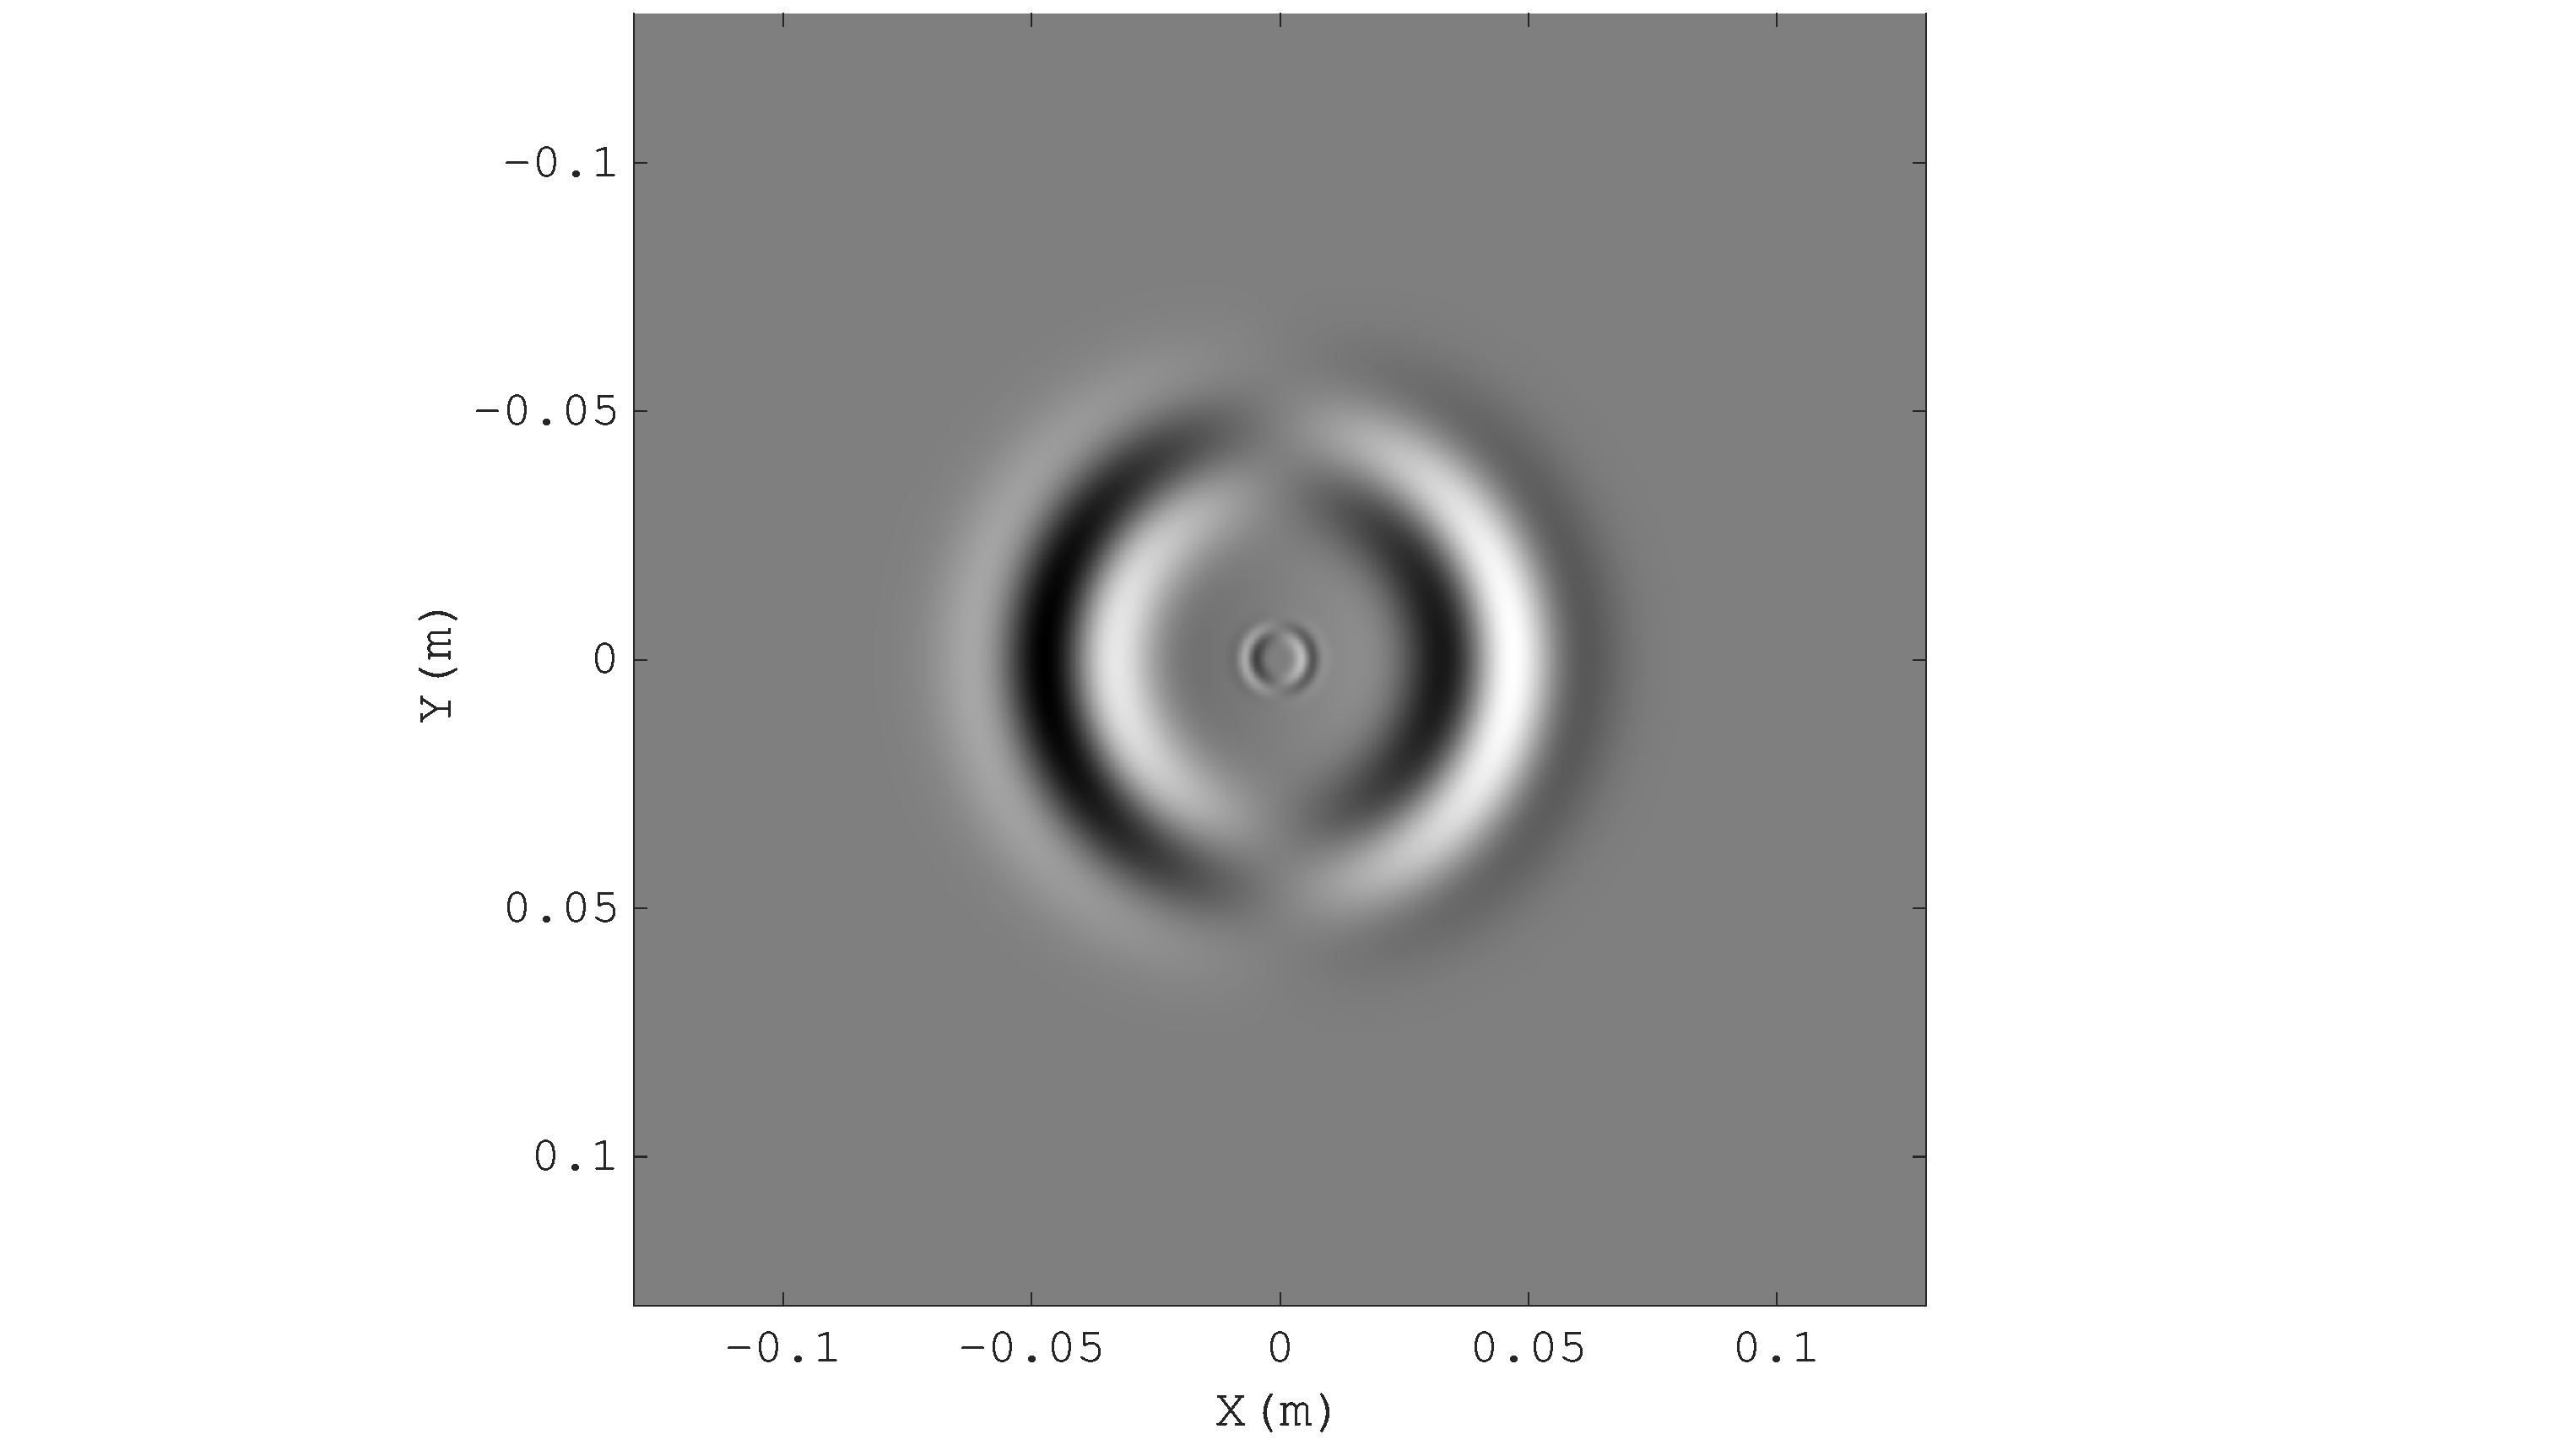
\includegraphics[draft=false,width=1.2\textwidth]{Figures/wave_alfa_s_05_zoom1}
\caption{}
\end{subfigure}
\hfill
\begin{subfigure}{0.5\linewidth}
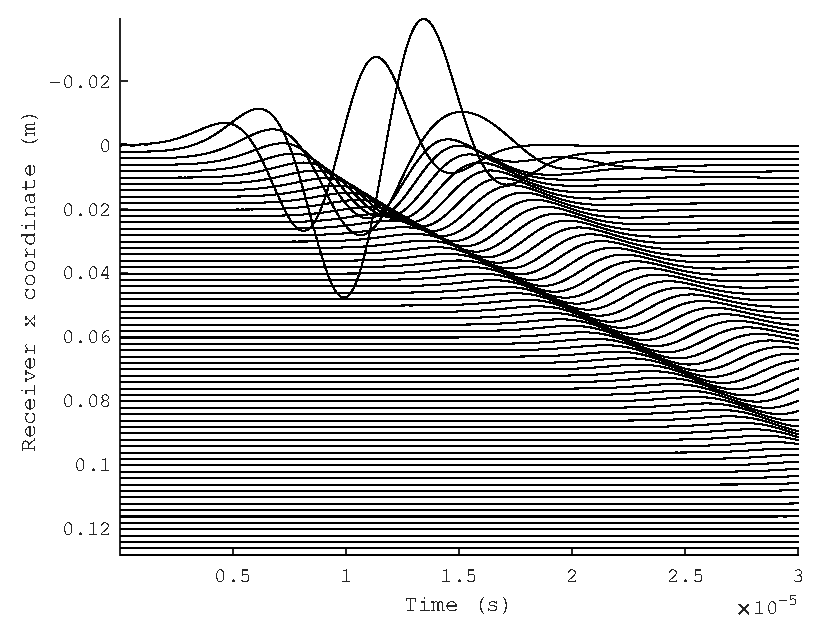
\includegraphics[draft=false,width=0.8\textwidth]{Figures/alfa_s_05_zoom}
\caption{}
\end{subfigure}%
\caption{A zoom snapshot at time $1\cdot10^{-5}s$  (a) and seismogram (b) of the mixture 
velocity $v^1$  for source of central frequency $f_{0} =10^{5} $ Hz and 
porosity 
parameter $\phi$=0.5.}
\label{fig:porosity 05 zoom}
\end{figure}
 A variation of the amplitudes for different parameters $\phi$ can also be 
 seen in Fig.\,\ref{fig:porosity different}, where the wavefield along the 
 $x$-direction for $y=0$ is presented. 
 \begin{figure}[!htbp]
	\begin{center}
		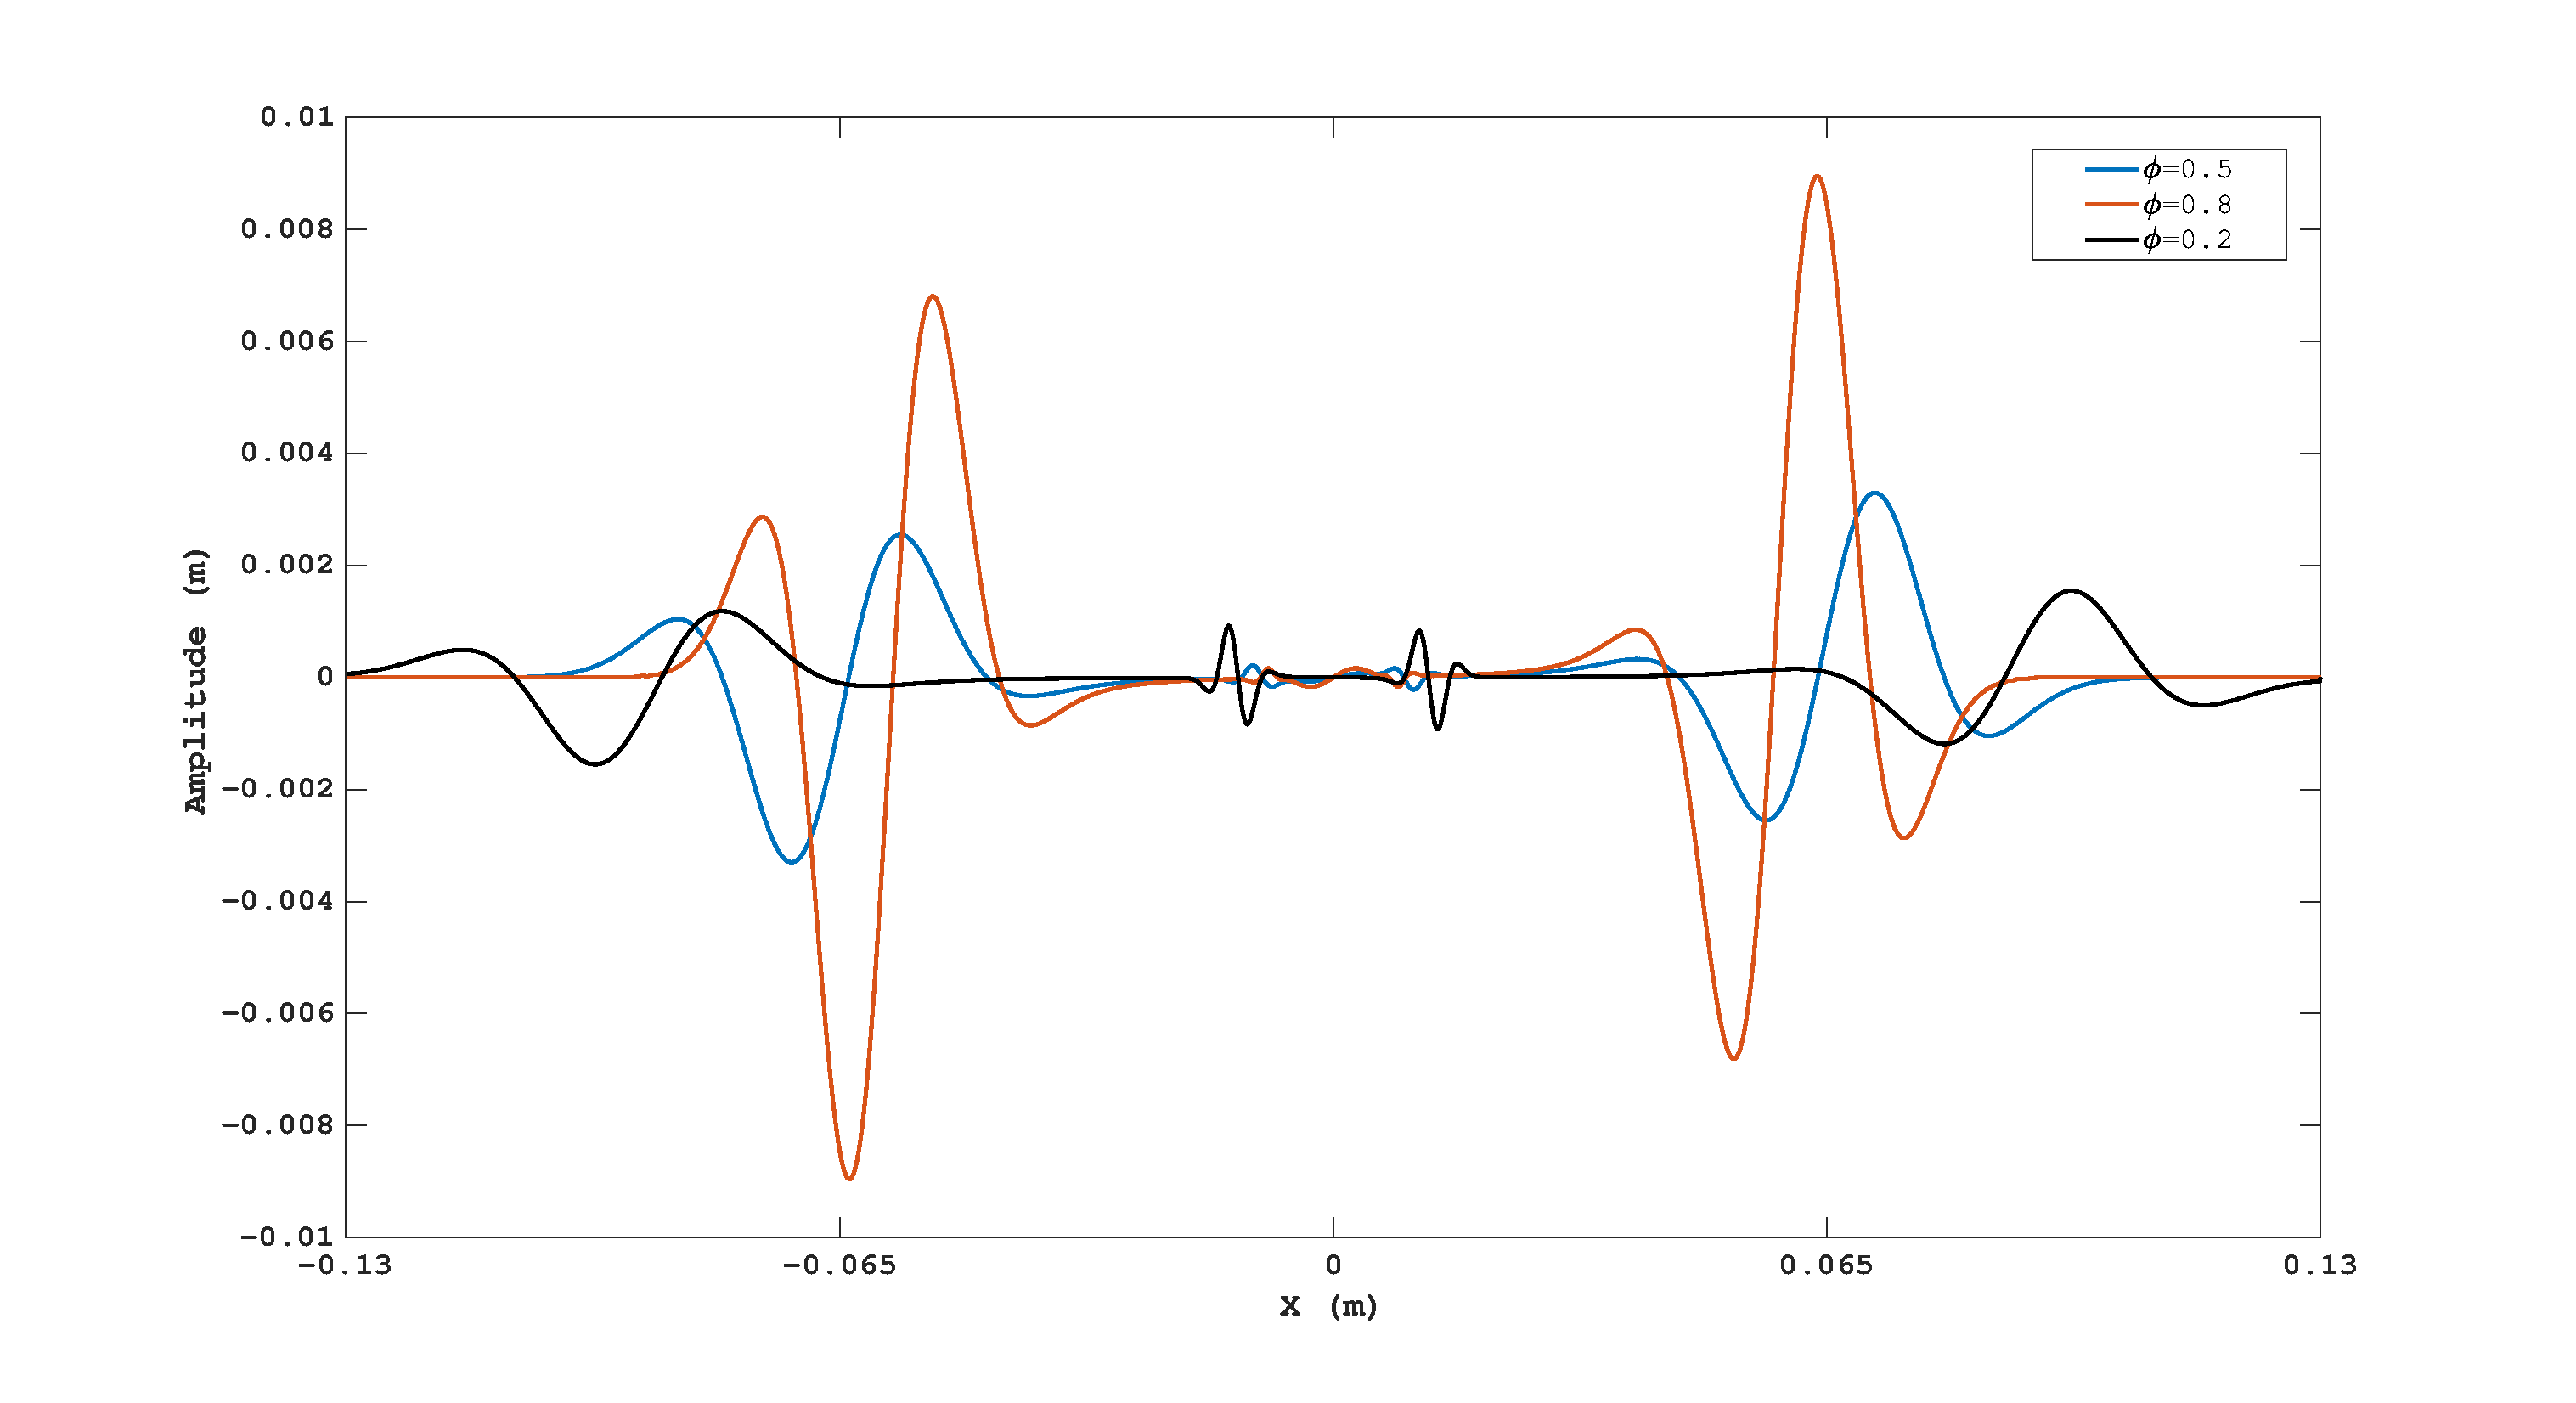
\includegraphics[draft=false,width=1.0\textwidth]{Figures/Compare_alfa}
	\end{center}
\caption{The wavefield distribution along the $x$-direction and $y=0$  at the 
time $2.1\cdot10^{-5}s$ of the mixture velocity $v^1$ for different values of 
$\phi$: $\phi=0.2$ (black), $\phi=0.5$ (blue), $\phi=0.8$ 
(red).}
\label{fig:porosity different}
\end{figure}

Summarizing  the numerical experiments from this section, one can conclude that 
by varying the porosity $\phi$ in system \eqref{stress.velocity}, it is 
possible to correctly describe three states of the medium: liquid, solid and 
poroelastic.

\subsection{Dependence on the friction $ \theta_2 $.}

In this section, we study the behavior and properties of the fast and slow 
P-waves, depending on the parameter $\theta_2$. This parameter is presented as 
a denominator on the right hand side of the second equation in system 
\eqref{stress.velocity}. By analogy with the Bio model, $\theta_2$ can be 
viewed as the friction parameter because it controls the interfacial friction 
in multiphase medium and leads to the wave dispersion and attenuation.

Consider the same homogeneous numerical model as in the previous sections with 
$ \theta_2$ equal to $3.36\cdot10^{-7}$ from Table\,\ref{tab:parameters}. Let 
us observe the behavior of the  P-waves if we twice increase or twice decrease 
this parameter. The Fig.\,\ref{fig:compare_friction}(a-c) shows snapshots of 
the mixture velocity $v^1$ for these three values of $ \theta_2$. It can be 
observed a significant wave amplitude variations only for slow P-wave. A more 
detailed variation of the amplitudes can be seen in 
Fig.\,\ref{fig:compare_friction_line}, where the wavefield along the 
$x$-direction 
at $y=0$ is presented. The analysis of this graph demonstrates an increase in 
the 
amplitude of  the slow P-wave with the increase $\theta_2$ 
and vice versa. We also observe a change in the waveform of slow waves, while 
the fast wave remains almost unchanged.

Summarizing  the numerical experiments from this section, one can conclude, 
that by varying the parameter $\theta_2$ in system \eqref{stress.velocity}, it 
is possible to affect the amplitude and  propagation velocity of the slow 
P-wave. One of the interesting applications, in our opinion, can be the 
solution of the inverse problem of determining the coefficient $\theta_2$ by 
analyzing the ratio of the amplitudes of the fast and slow waves in a field 
experiment.
\begin{figure}[!htbp]
\begin{subfigure}{0.3\linewidth}
\centering
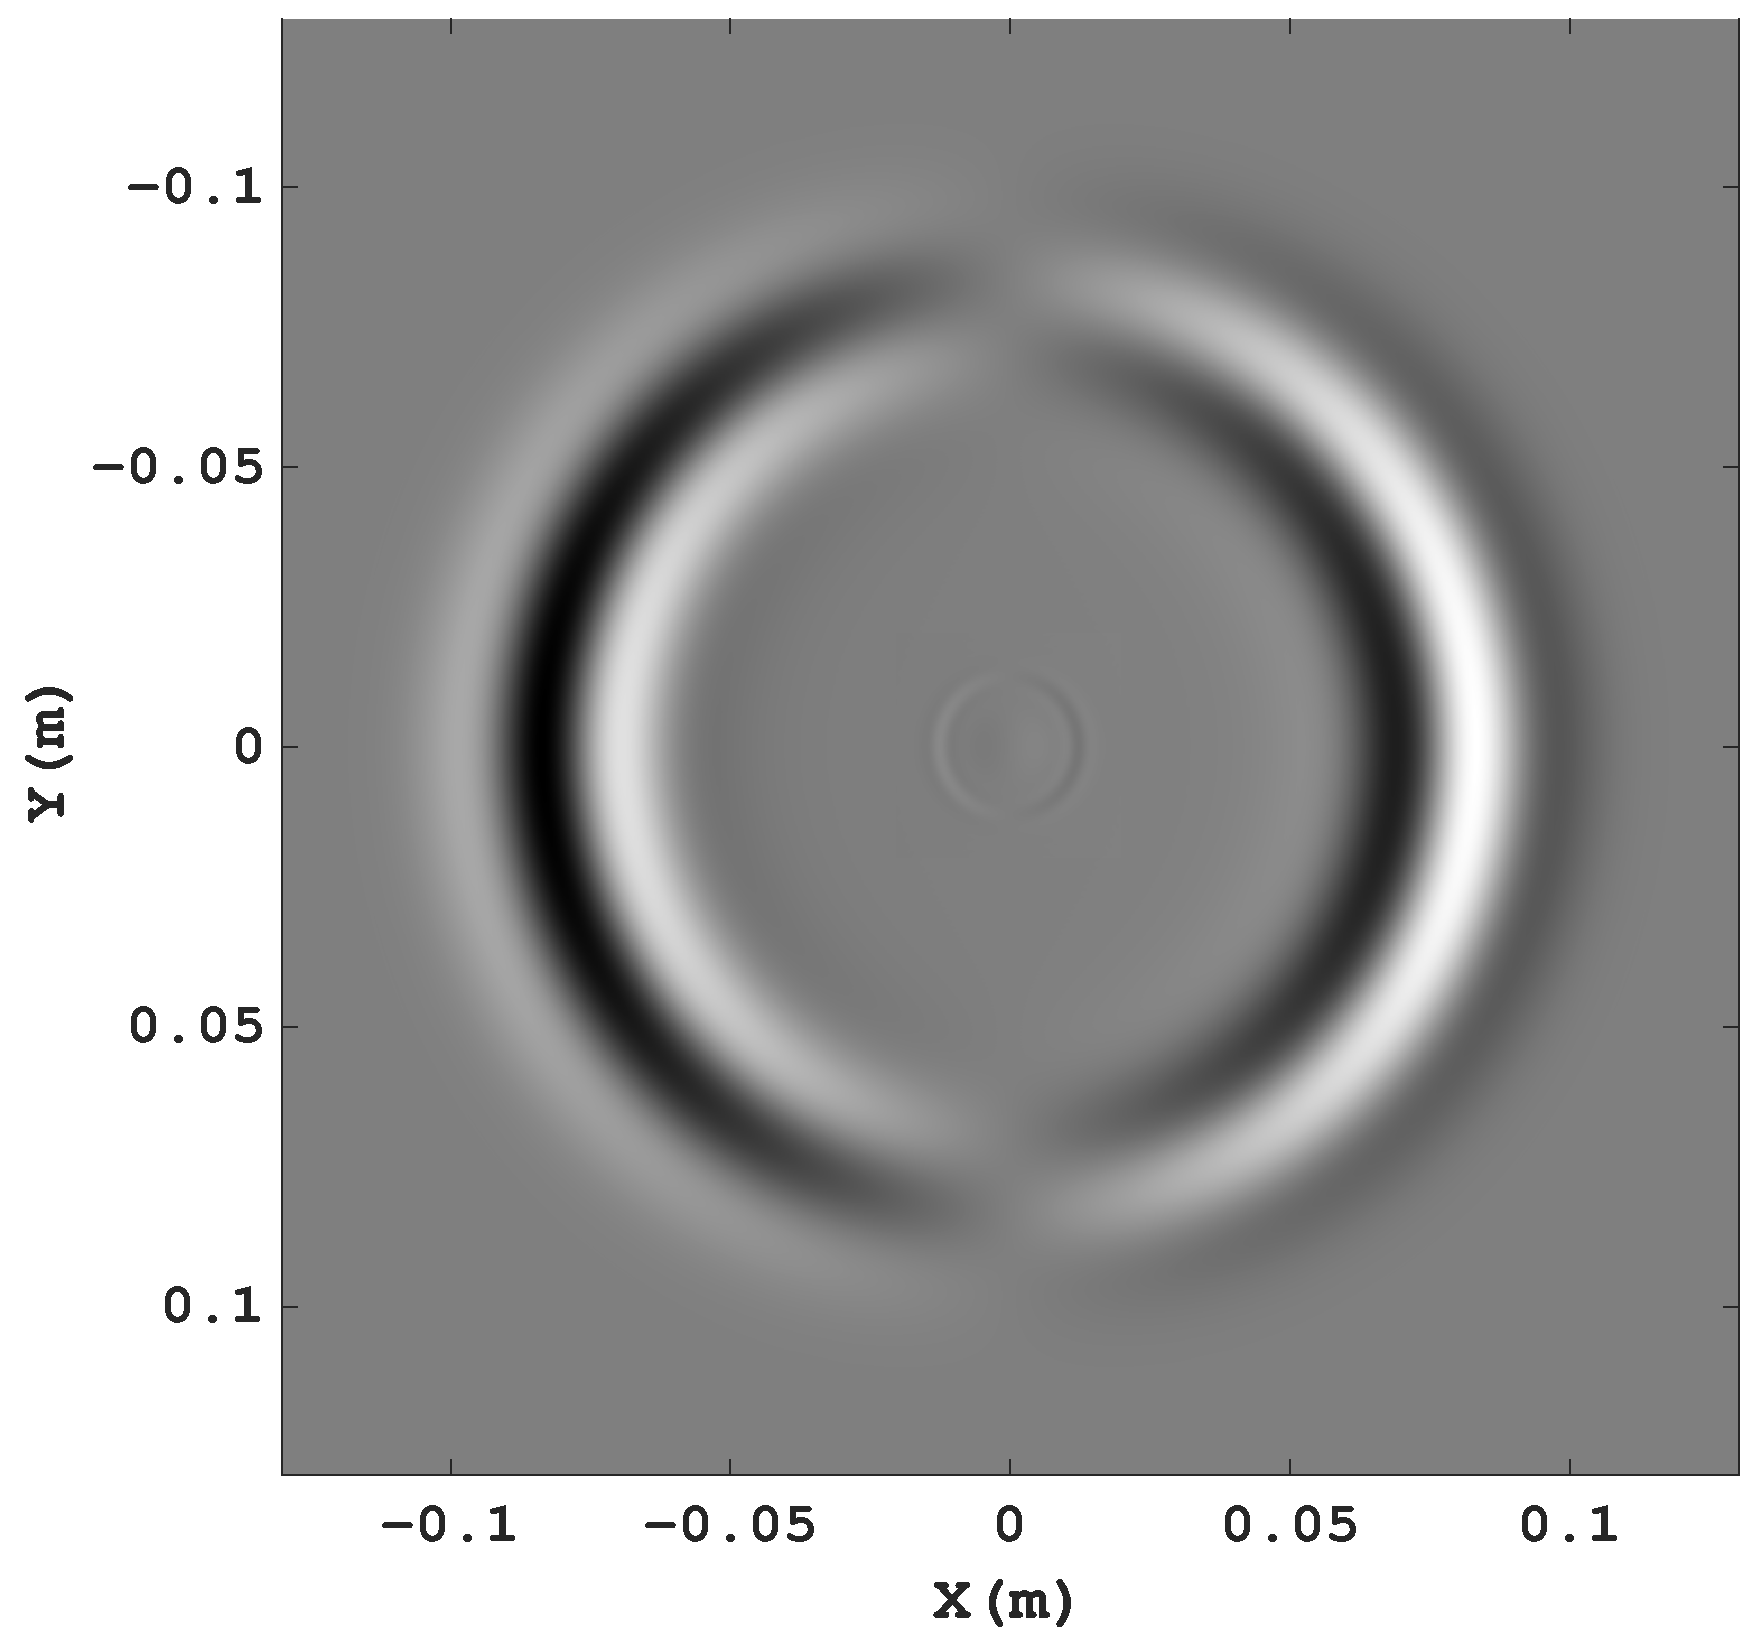
\includegraphics[draft=false,width=1\textwidth]{Figures/Xi_11_new}
\caption{$ \quad\quad \theta_2=3.36\cdot10^{-7} $}
\end{subfigure}
\hfill
\begin{subfigure}{0.3\linewidth}
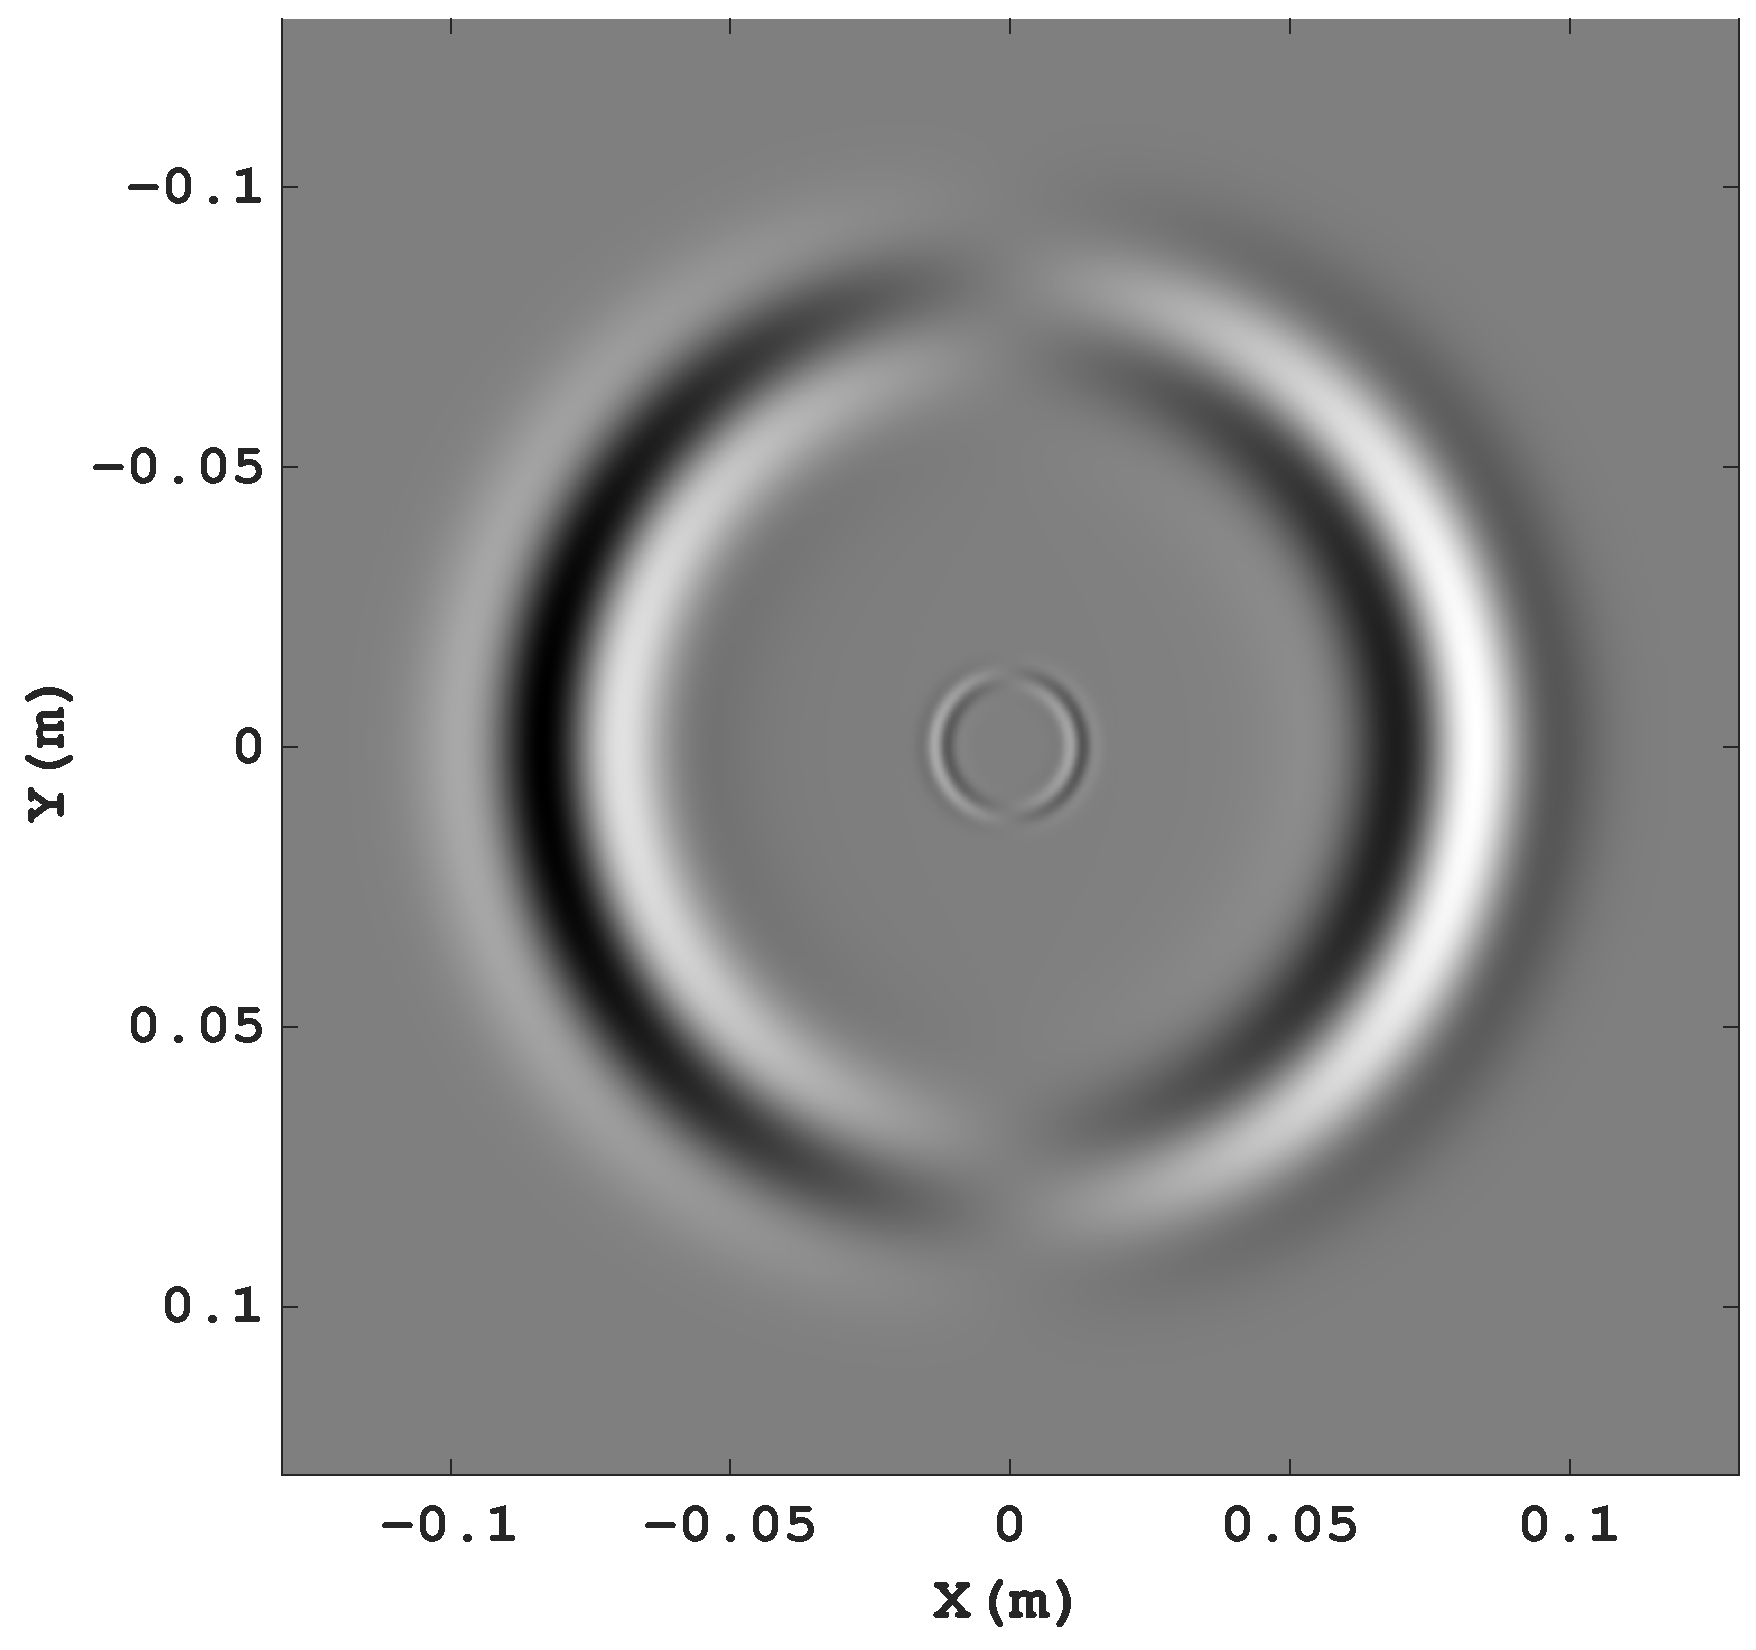
\includegraphics[draft=false,width=1\textwidth]{Figures/Xi_21_new}
\caption{$ \quad\quad \theta_2=2\cdot3.36\cdot10^{-7} $}
\end{subfigure}%
\hfill
\begin{subfigure}{0.3\linewidth}
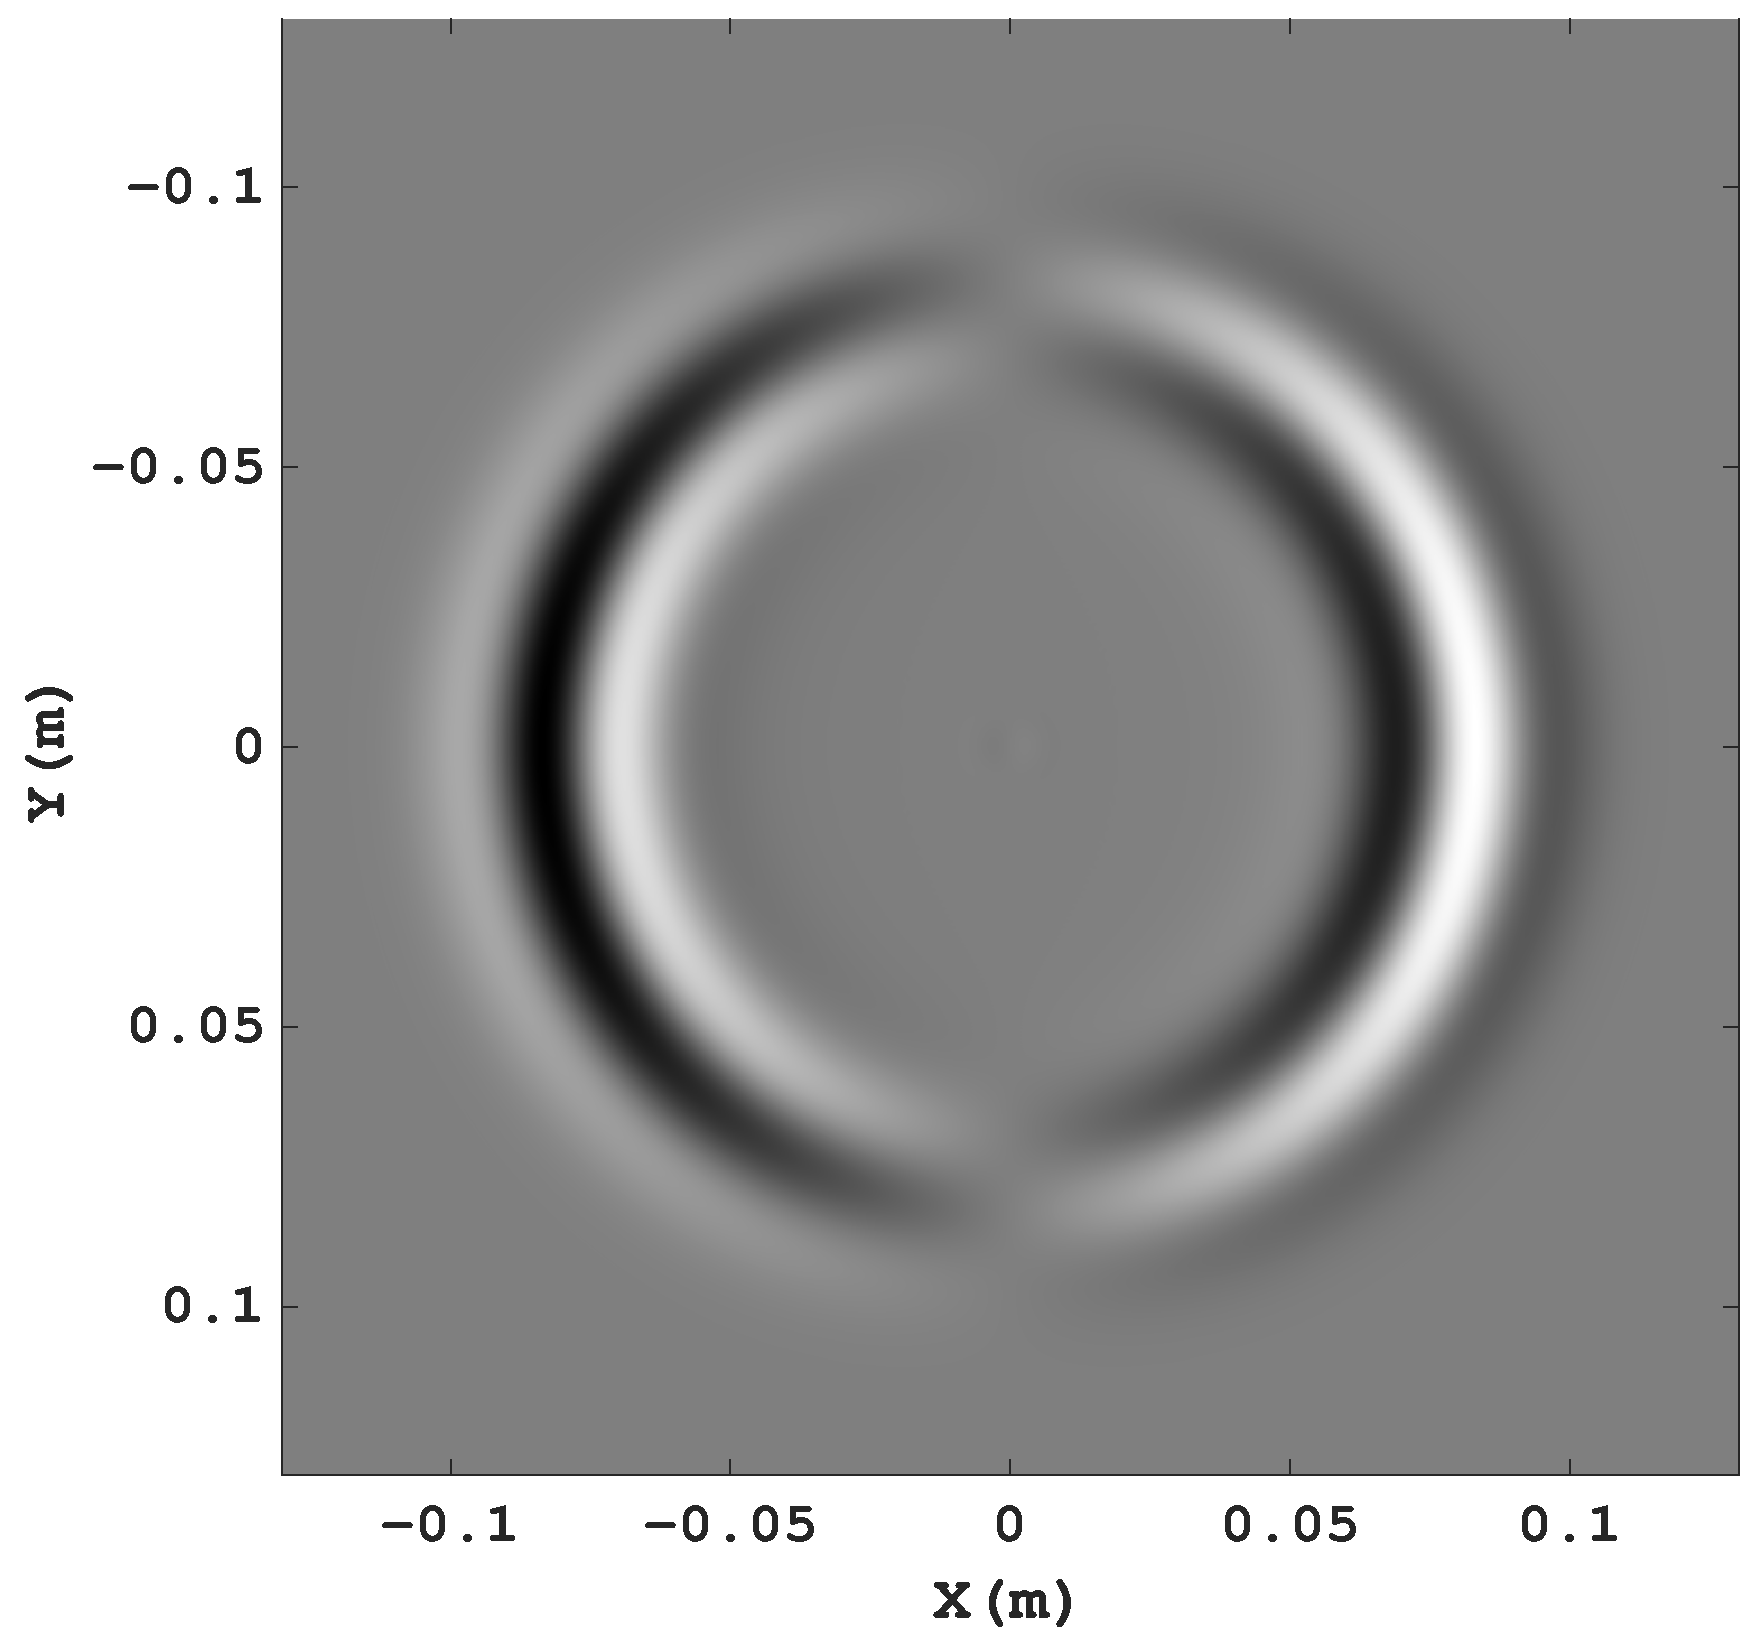
\includegraphics[draft=false,width=1\textwidth]{Figures/Xi_31_new}
\caption{$ \quad\quad \theta_2=1/2\cdot3.36\cdot10^{-7} $}
\end{subfigure}%
\caption{Snapshots at time $2.1\cdot10^{-5}s$ of the mixture velocity $v^1$ for different values of $ \theta_2 $.}
\label{fig:compare_friction}
\end{figure}
\begin{figure}[!htbp]
	\begin{center}
		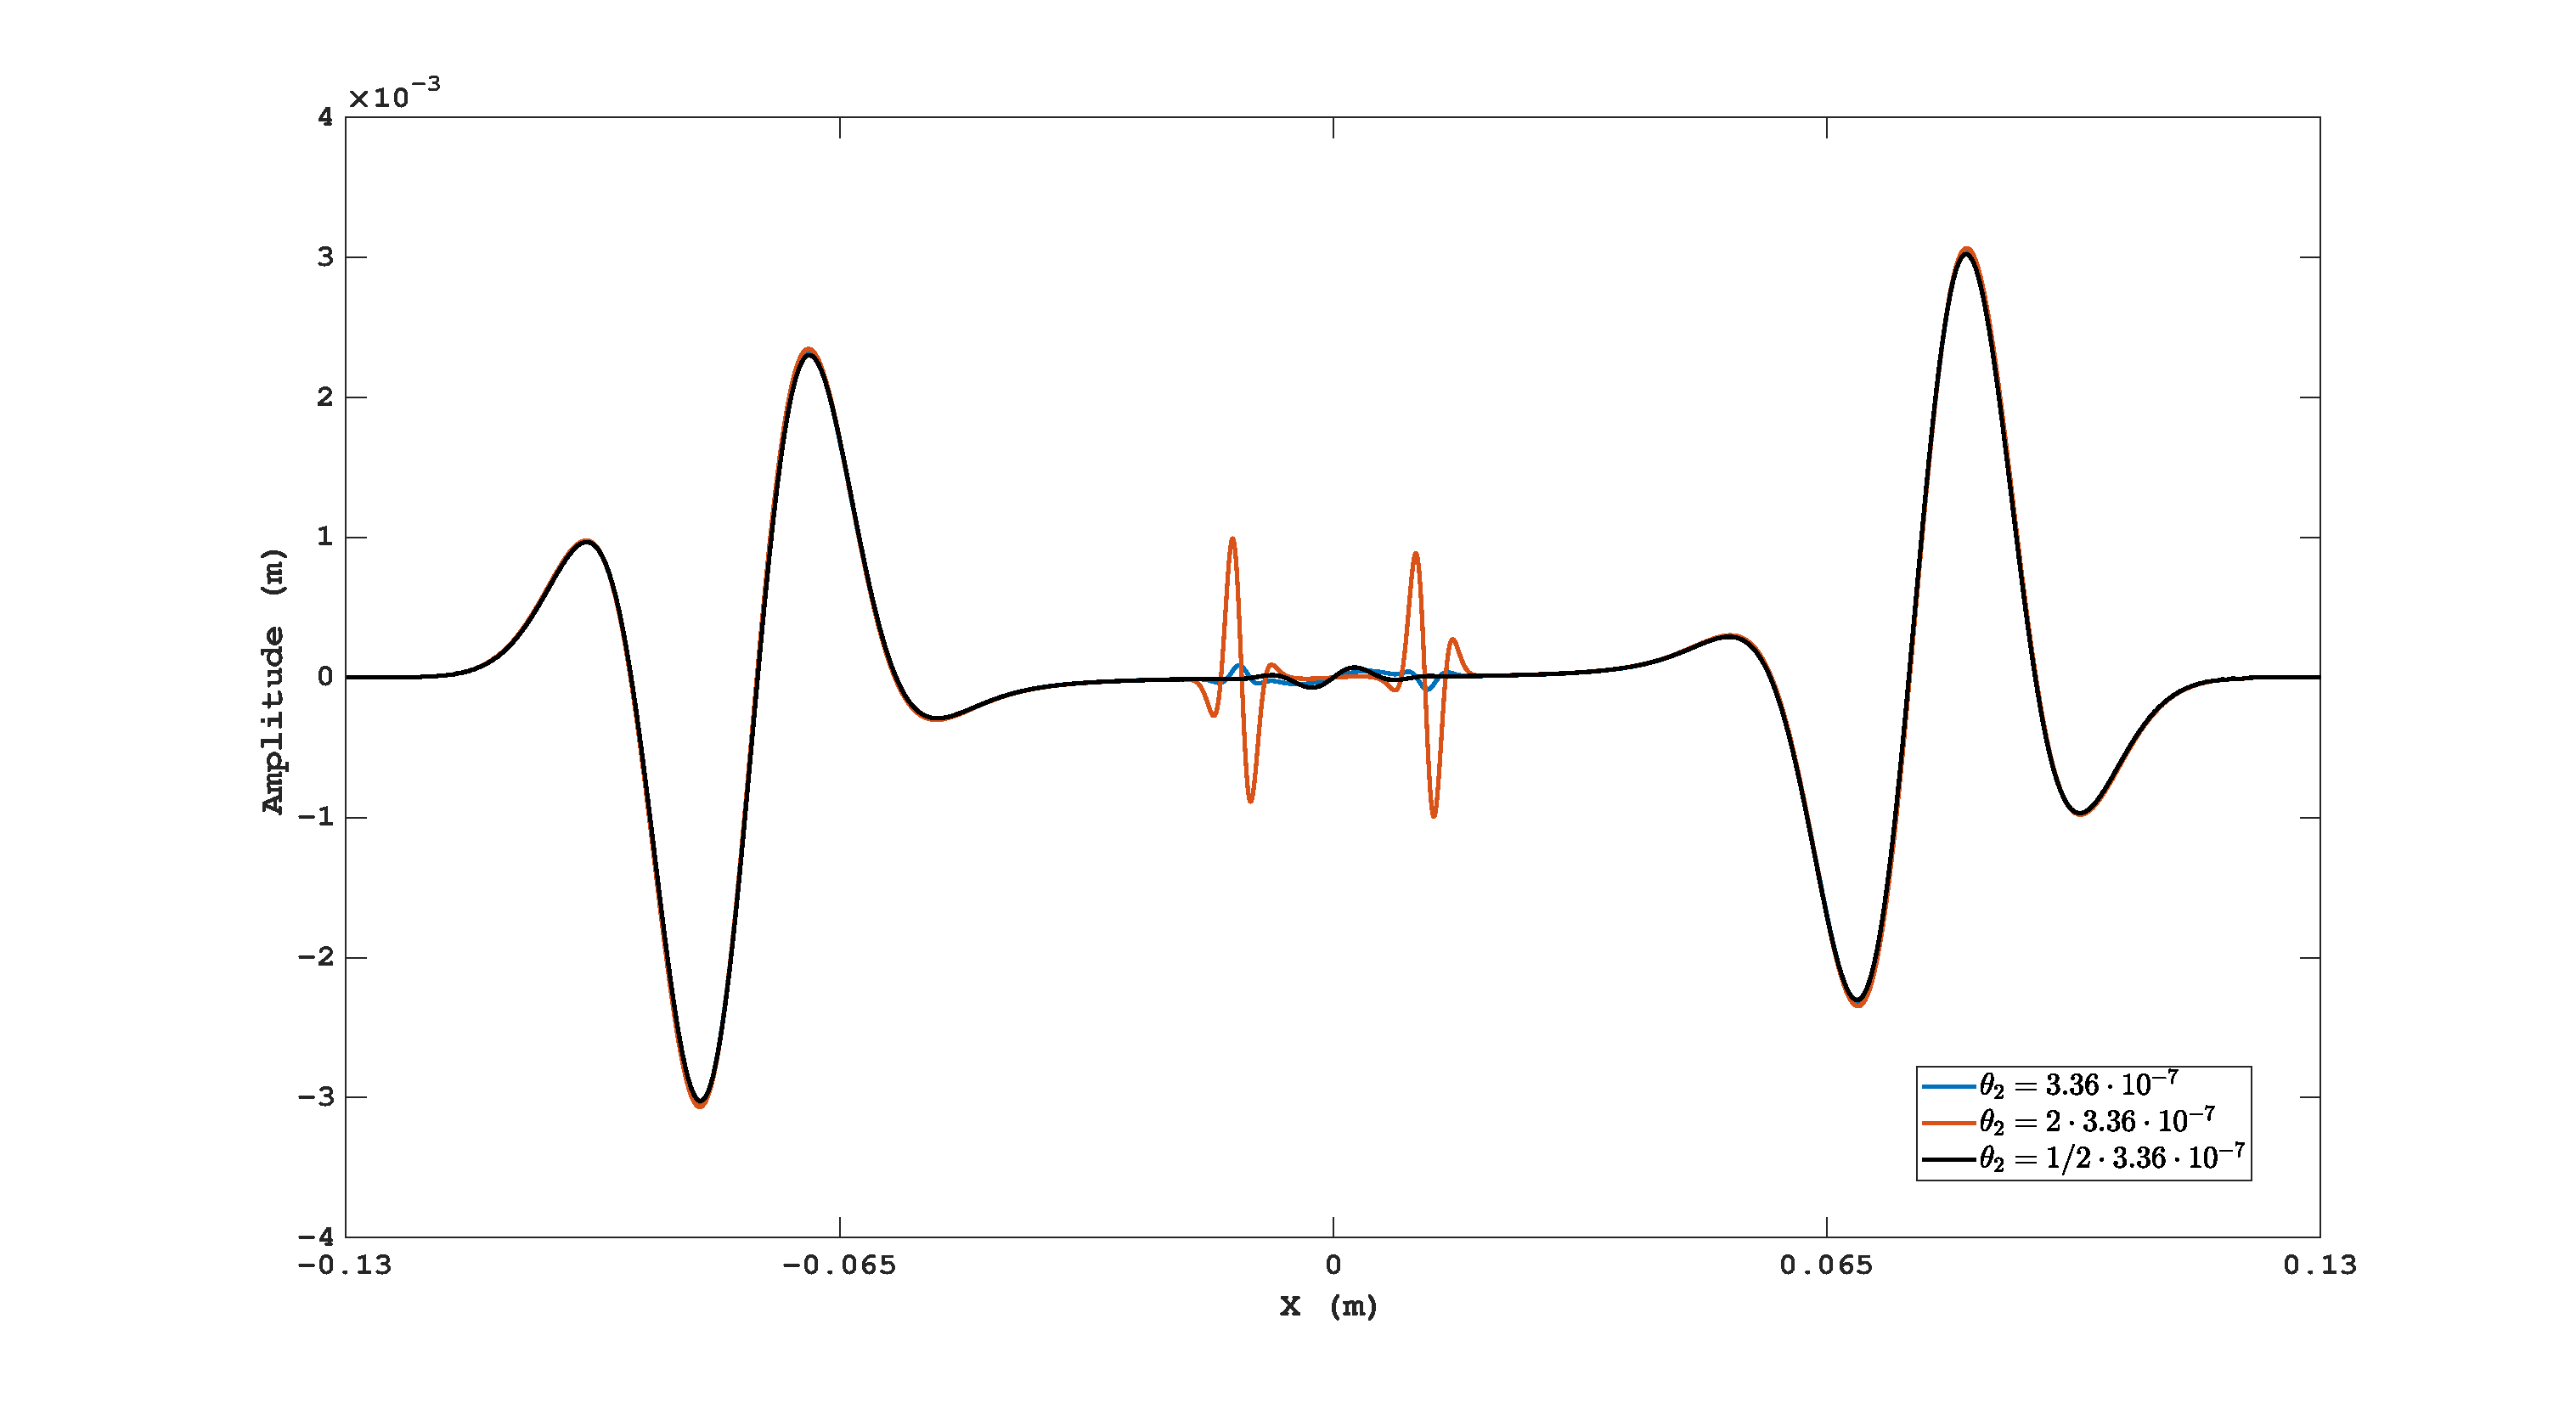
\includegraphics[draft=false,width=1.0\textwidth]{Figures/Compare_Xi_1}
	\end{center}
	\caption{A comparison at time $2.1\cdot10^{-5}$ s of the mixture velocity 
	$v^1$ for different values of $ \theta_2 $: $ \theta_2 
	=3.36\cdot10^{-7}$ (blue), $ \theta_2=2 \cdot 3.36\cdot10^{-7} $ (red), $ 
	\theta_2=1/2 \cdot 3.36\cdot10^{-7} $ (black).}
	\label{fig:compare_friction_line}
\end{figure}

\subsection{Dependence on the frequency $f_{0}$.}\label{sec.frequency}

In this section, we study the dispersion of the wave velocity depending on the 
source 
peak frequency $f_{0}$  based on of the same homogeneous numerical model 
with 
parameters from Table \ref{tab:parameters} as in the previous sections. 
The dispersion curves in Fig.\,\ref{fig:diff.grain.modulus} show the main 
velocity changes in the range of $10^{4}-10^{6}$ Hz. Because of a difference in 
three order of magnitude in the frequency range, the comparison will be done 
not 
within the framework of one computational domain but for three different 
domains. Thus, we use the 10 orders of magnitude scaling of the both space and 
time. Fig.\,\ref{fig:compare_frewuency} presents 
snapshots and Fig.\,\ref{fig:compare_frewuency_trace} presents seismograms of 
the mixture velocity $v^1$ for different frequencies. For each time frequency, 
a snapshot is recorded at the time $5/{f_{0}}$ (including the shift wavelet 
delay $1/{f_{0}}$) for the square domains with the side of $ 5 $ m (for 
$f_{0}=10^{4}$), $0.5$  m (for 
$f_{0}=10^{5}$) and $0.05$  m (for $f_{0}=10^{6}$). The time 
and size are chosen in such a way that in the isotropic elastic case 
we can obtain three identical snapshots. As it is expected for the poroelastic 
case, 
we 
observe wavefield differences which are most clearly seen in seismograms: the 
lower the frequency, the stronger the dispersion and attenuation of the slow 
P-wave. 
%To estimate the phase velocity and attenuation of a slow wave, we use 
%the spectral ratio technique 
%\cite{Gurevich2015}, \cite{Caspari2019}
%and estimate the quality factor $Q=2.12$, the 
%phase velocity $v_{p}=420 $ m/s for the frequency $f_{0}=10^{5}$ Hz and $Q=10$, 
%the phase velocity $v_{p}=670 $ m/s  for the frequency $f_{0}=10^{6}$ Hz. 
To estimate the phase velocity, we use 
the spectral ratio technique 
\cite{Gurevich2015}, \cite{Caspari2019}
and obtain the 
phase velocity $v_{p}=420 $ m/s for the frequency $f_{0}=10^{5}$ Hz and
$v_{p}=670 $ m/s  for the frequency $f_{0}=10^{6}$ Hz. 
It is not possible to make 
similar estimation for the frequency $f_{0}=10^{4}$ due to a low amplitude of slow wave. We 
can conclude that the attenuation of a slow P-wave is sufficiently strong even 
for high frequencies.
\begin{figure}[!htbp]
\begin{subfigure}{0.3\linewidth}
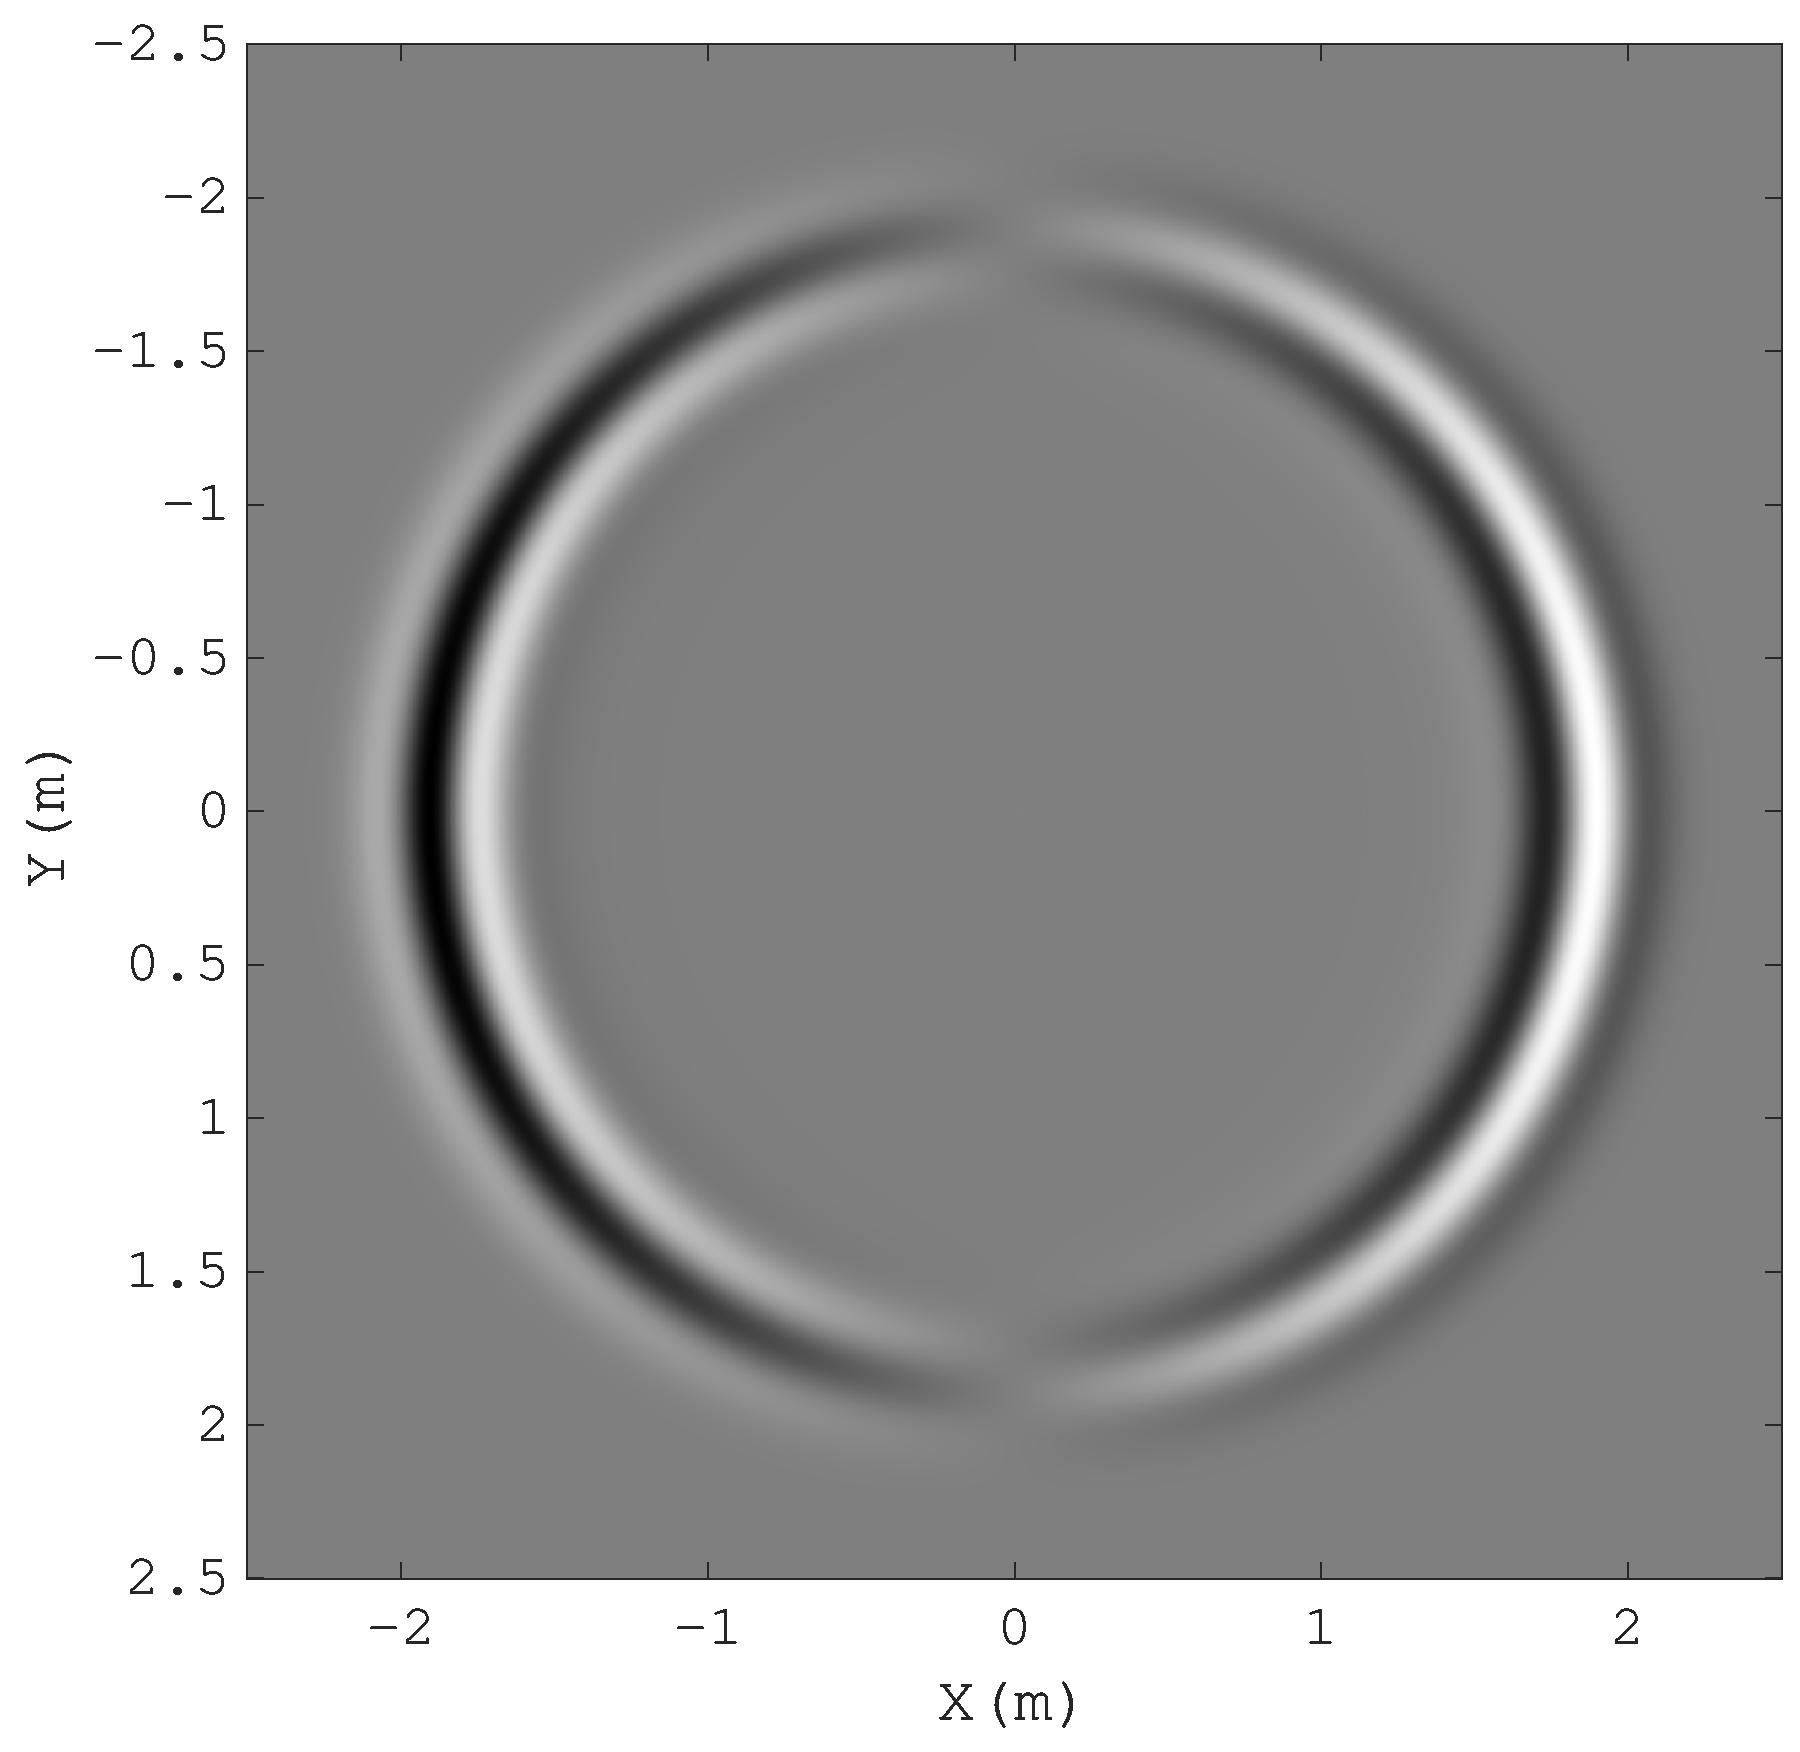
\includegraphics[draft=false,width=1\textwidth]{Figures/frec_big_10_4}
\caption{$\quad\quad f_0=10^{4} $}
\end{subfigure}
\hfill
\begin{subfigure}{0.3\linewidth}
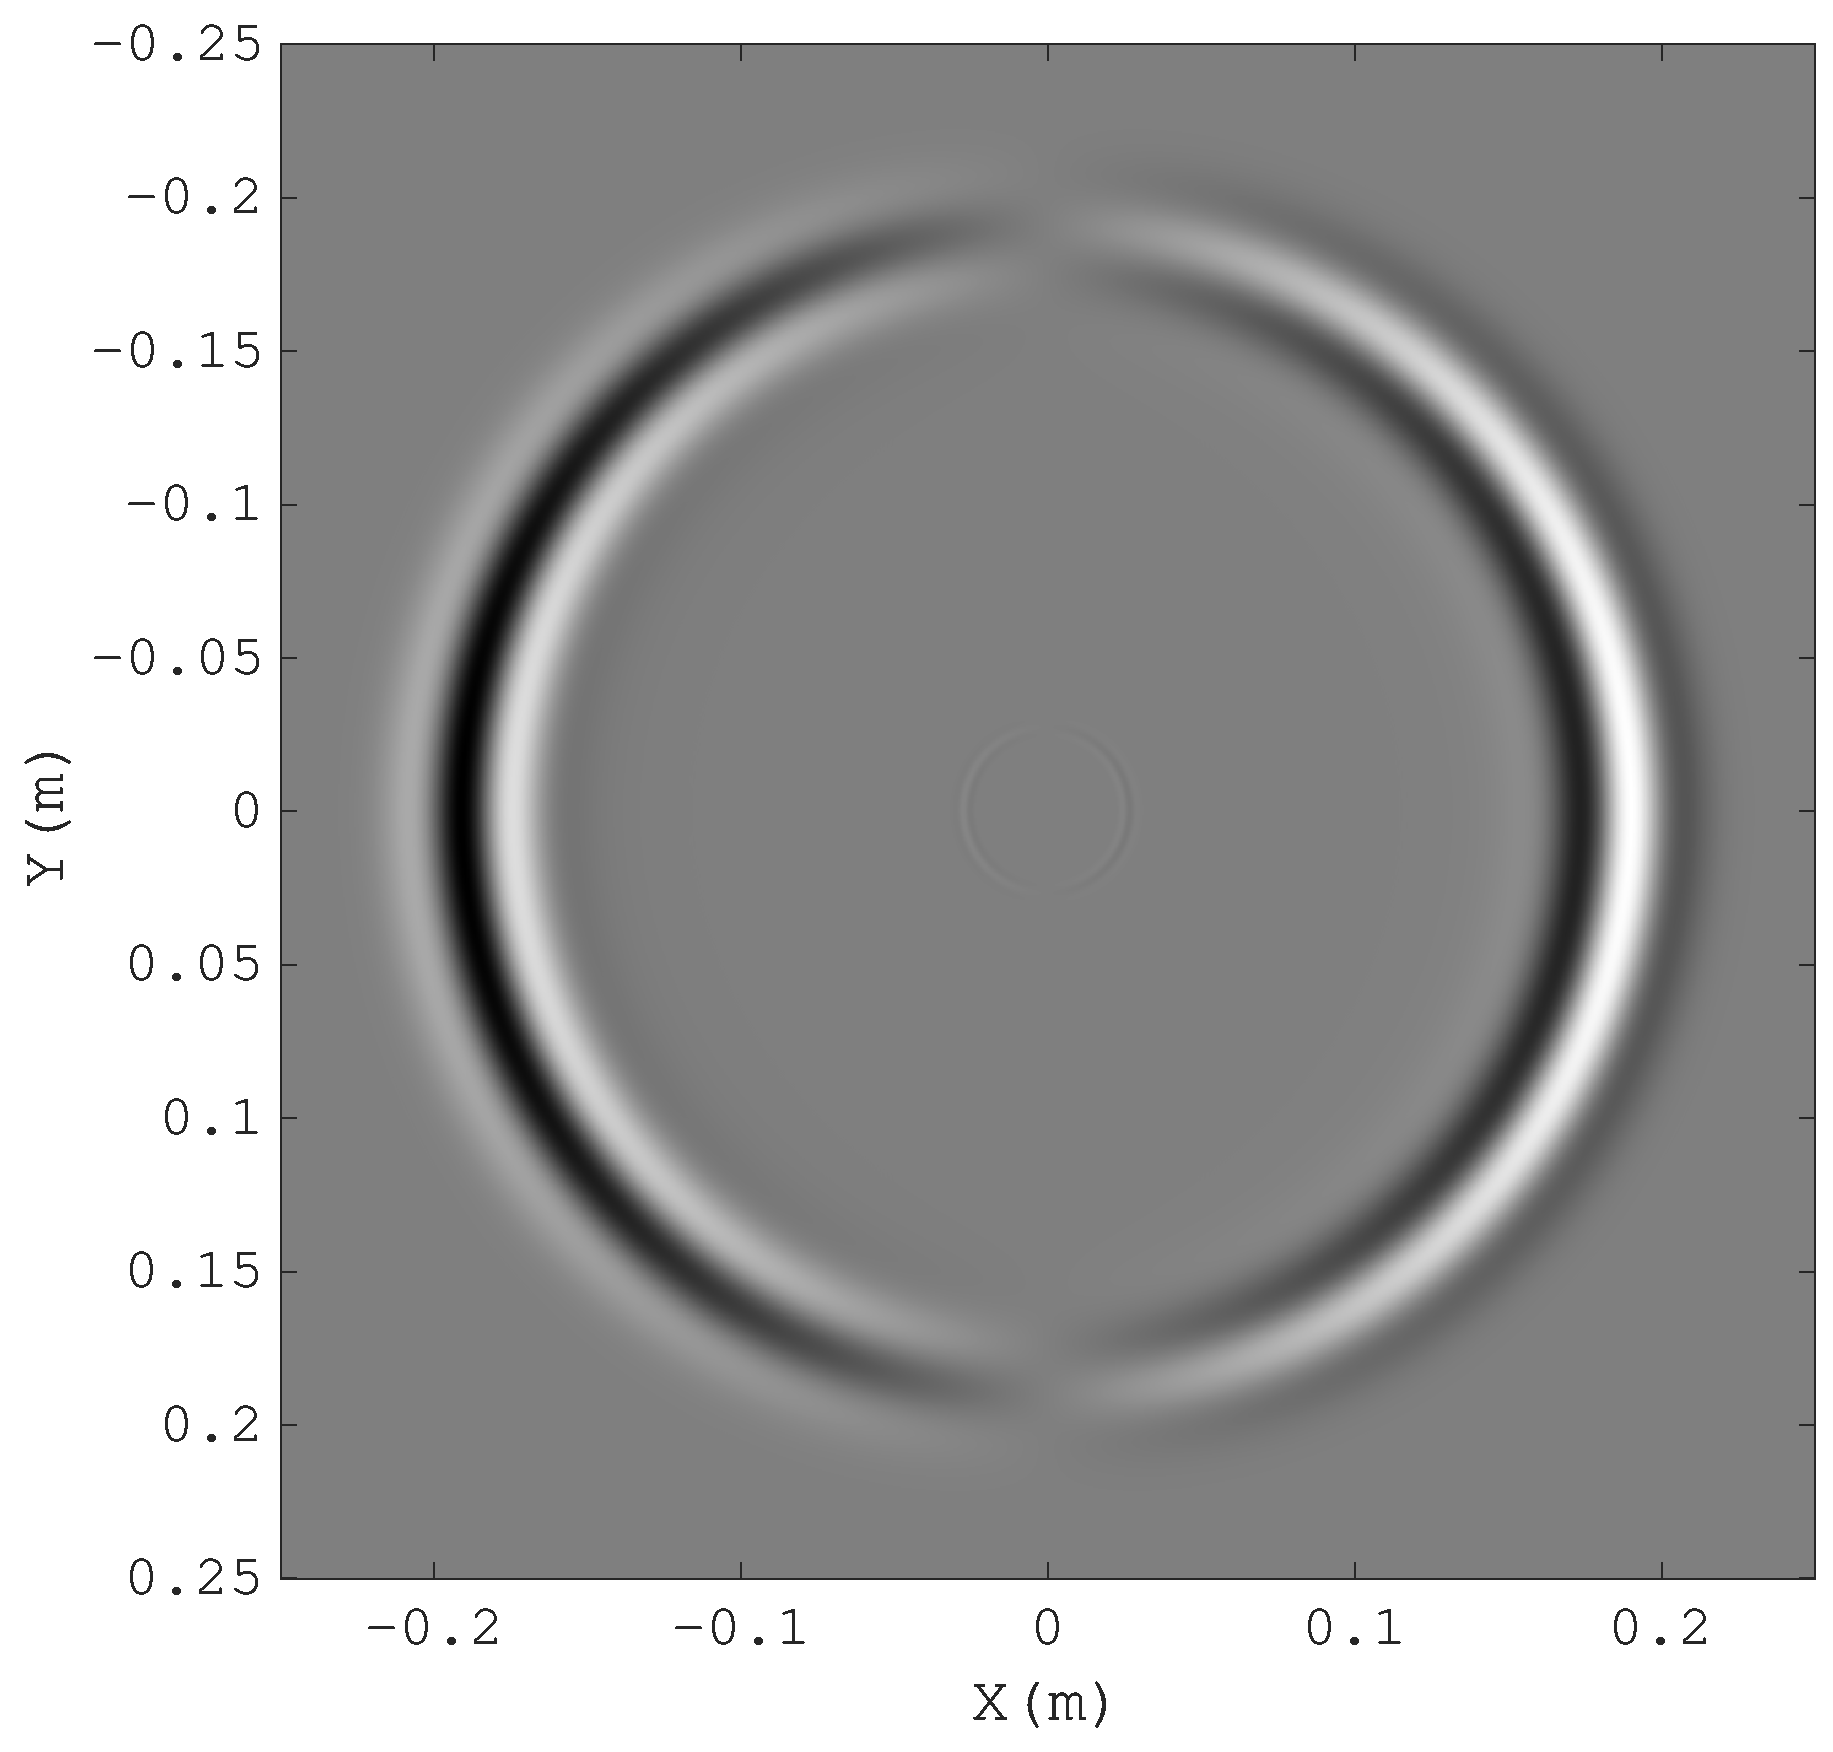
\includegraphics[draft=false,width=1\textwidth]{Figures/frec_big_10_5}
\caption{$\quad\quad f_0=10^{5} $}
\end{subfigure}%
\hfill
\begin{subfigure}{0.3\linewidth}
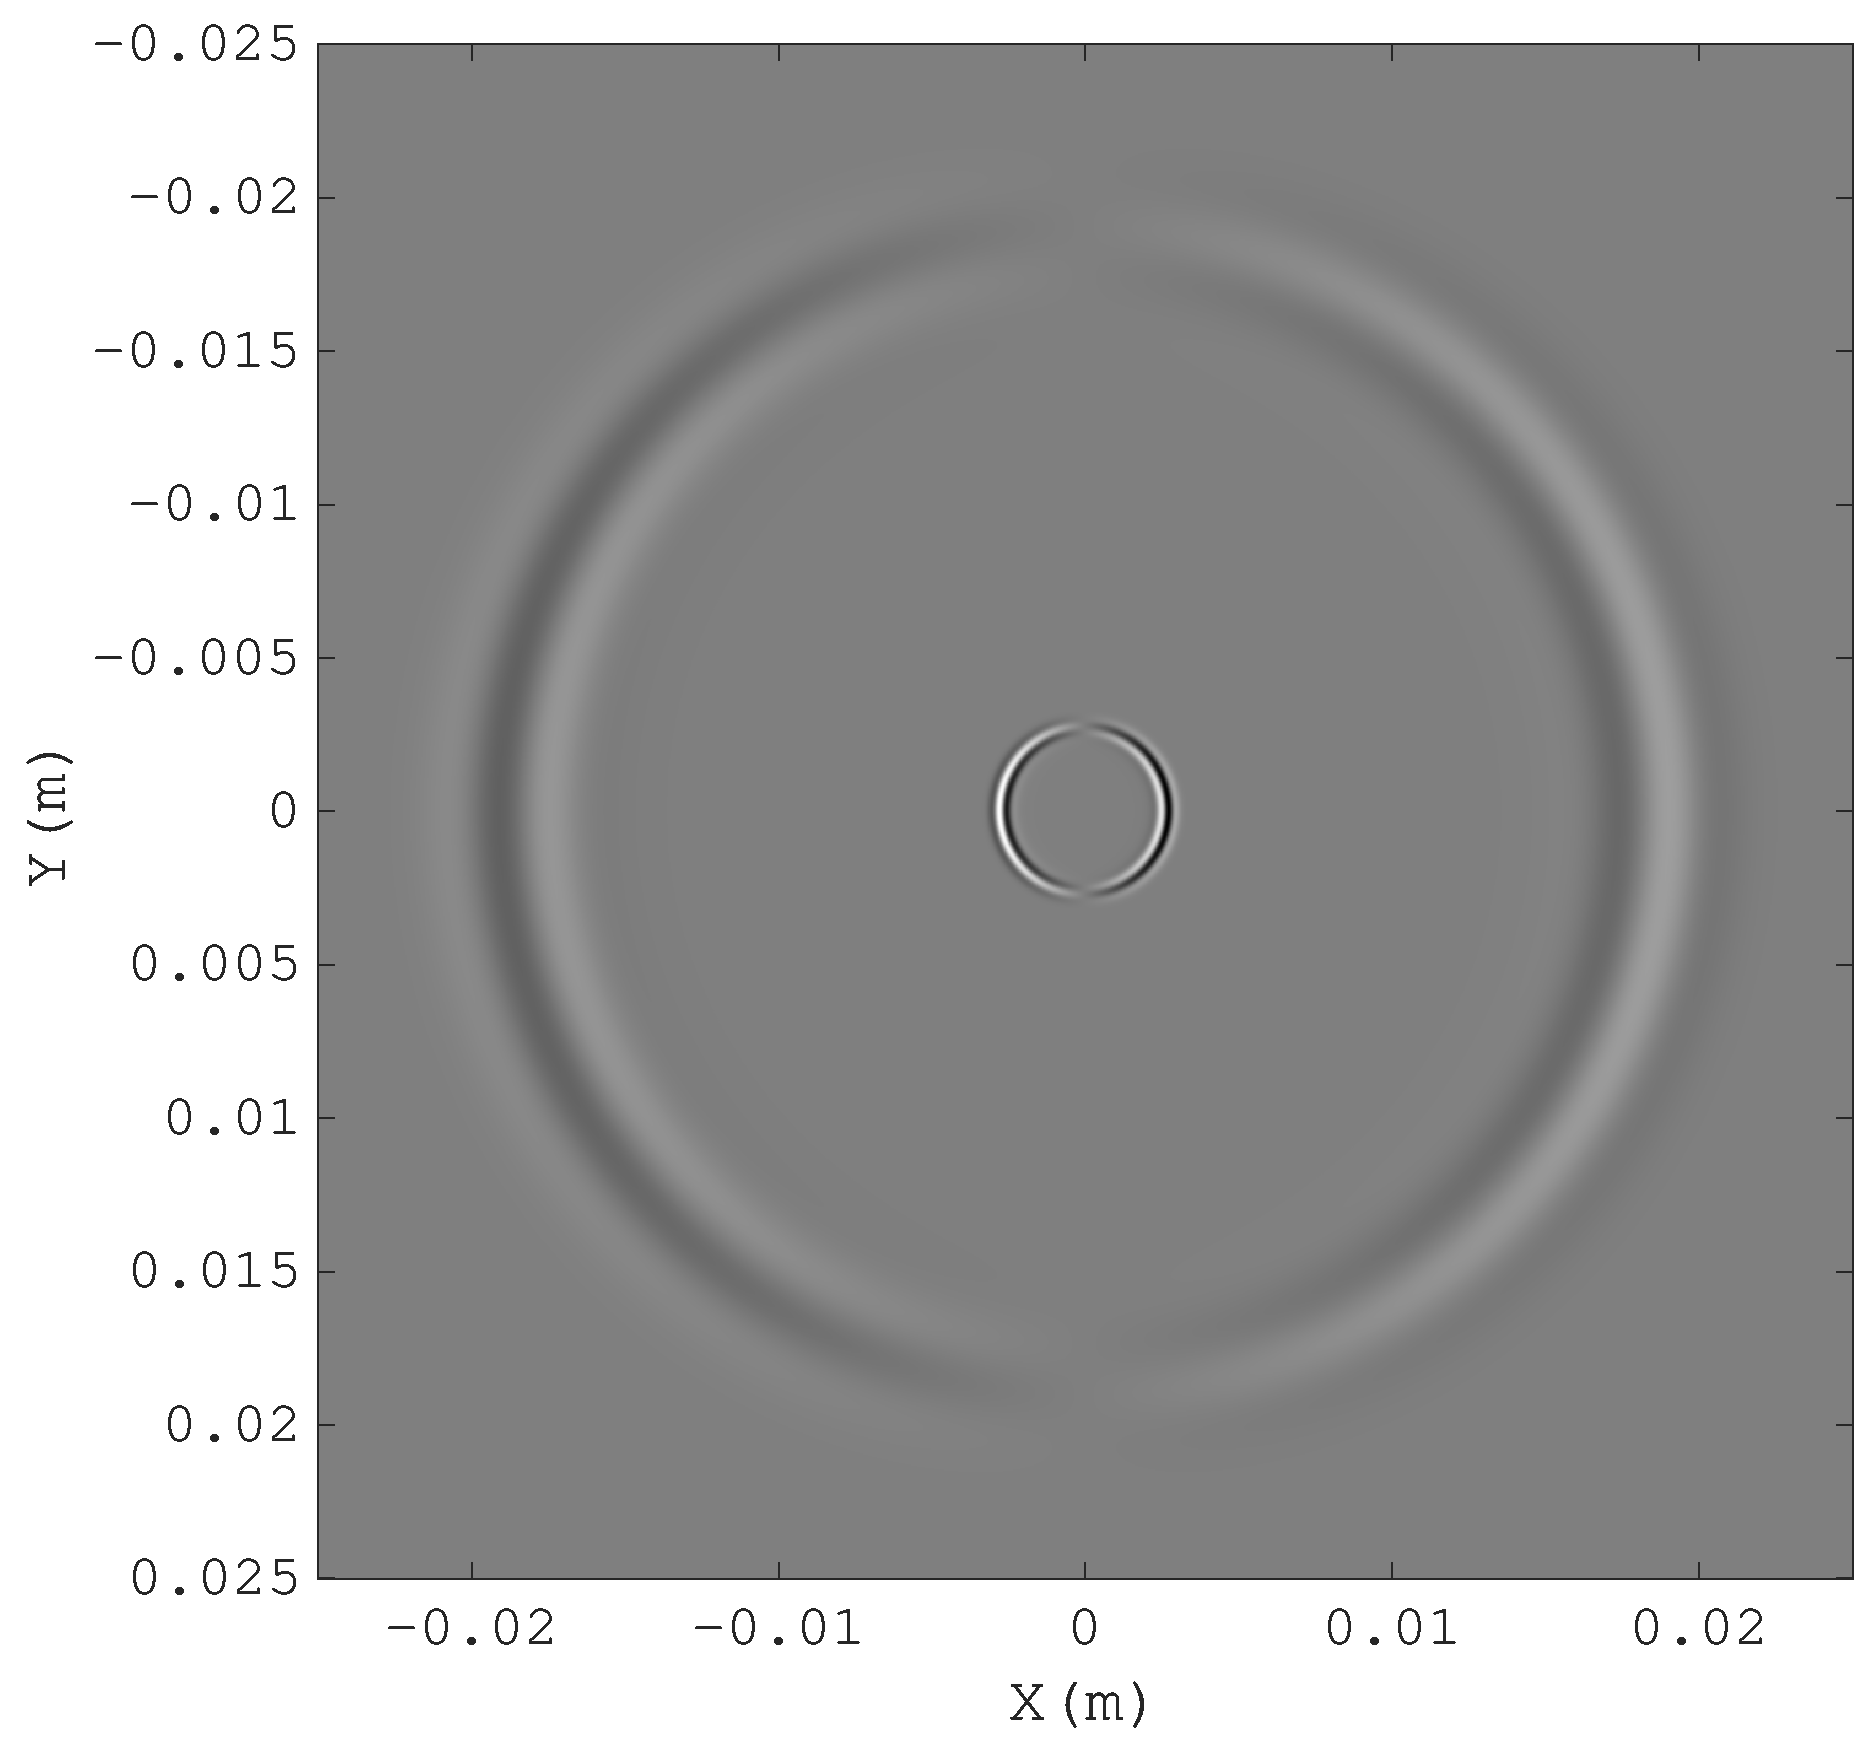
\includegraphics[draft=false,width=1\textwidth]{Figures/frec_big_10_6}
\caption{$\quad\quad f_0=10^{6} $}
\end{subfigure}%
\caption{  Snapshots of the mixture velocity $v^1$ for different frequencies: 
$f_0=10^{4}$ Hz (a), $f_0=10^{5}$ Hz (b), $f_0=10^{6}$ Hz (c) .  }
\label{fig:compare_frewuency}
\end{figure}

\begin{figure}[!htbp]
\begin{subfigure}{0.3\linewidth}
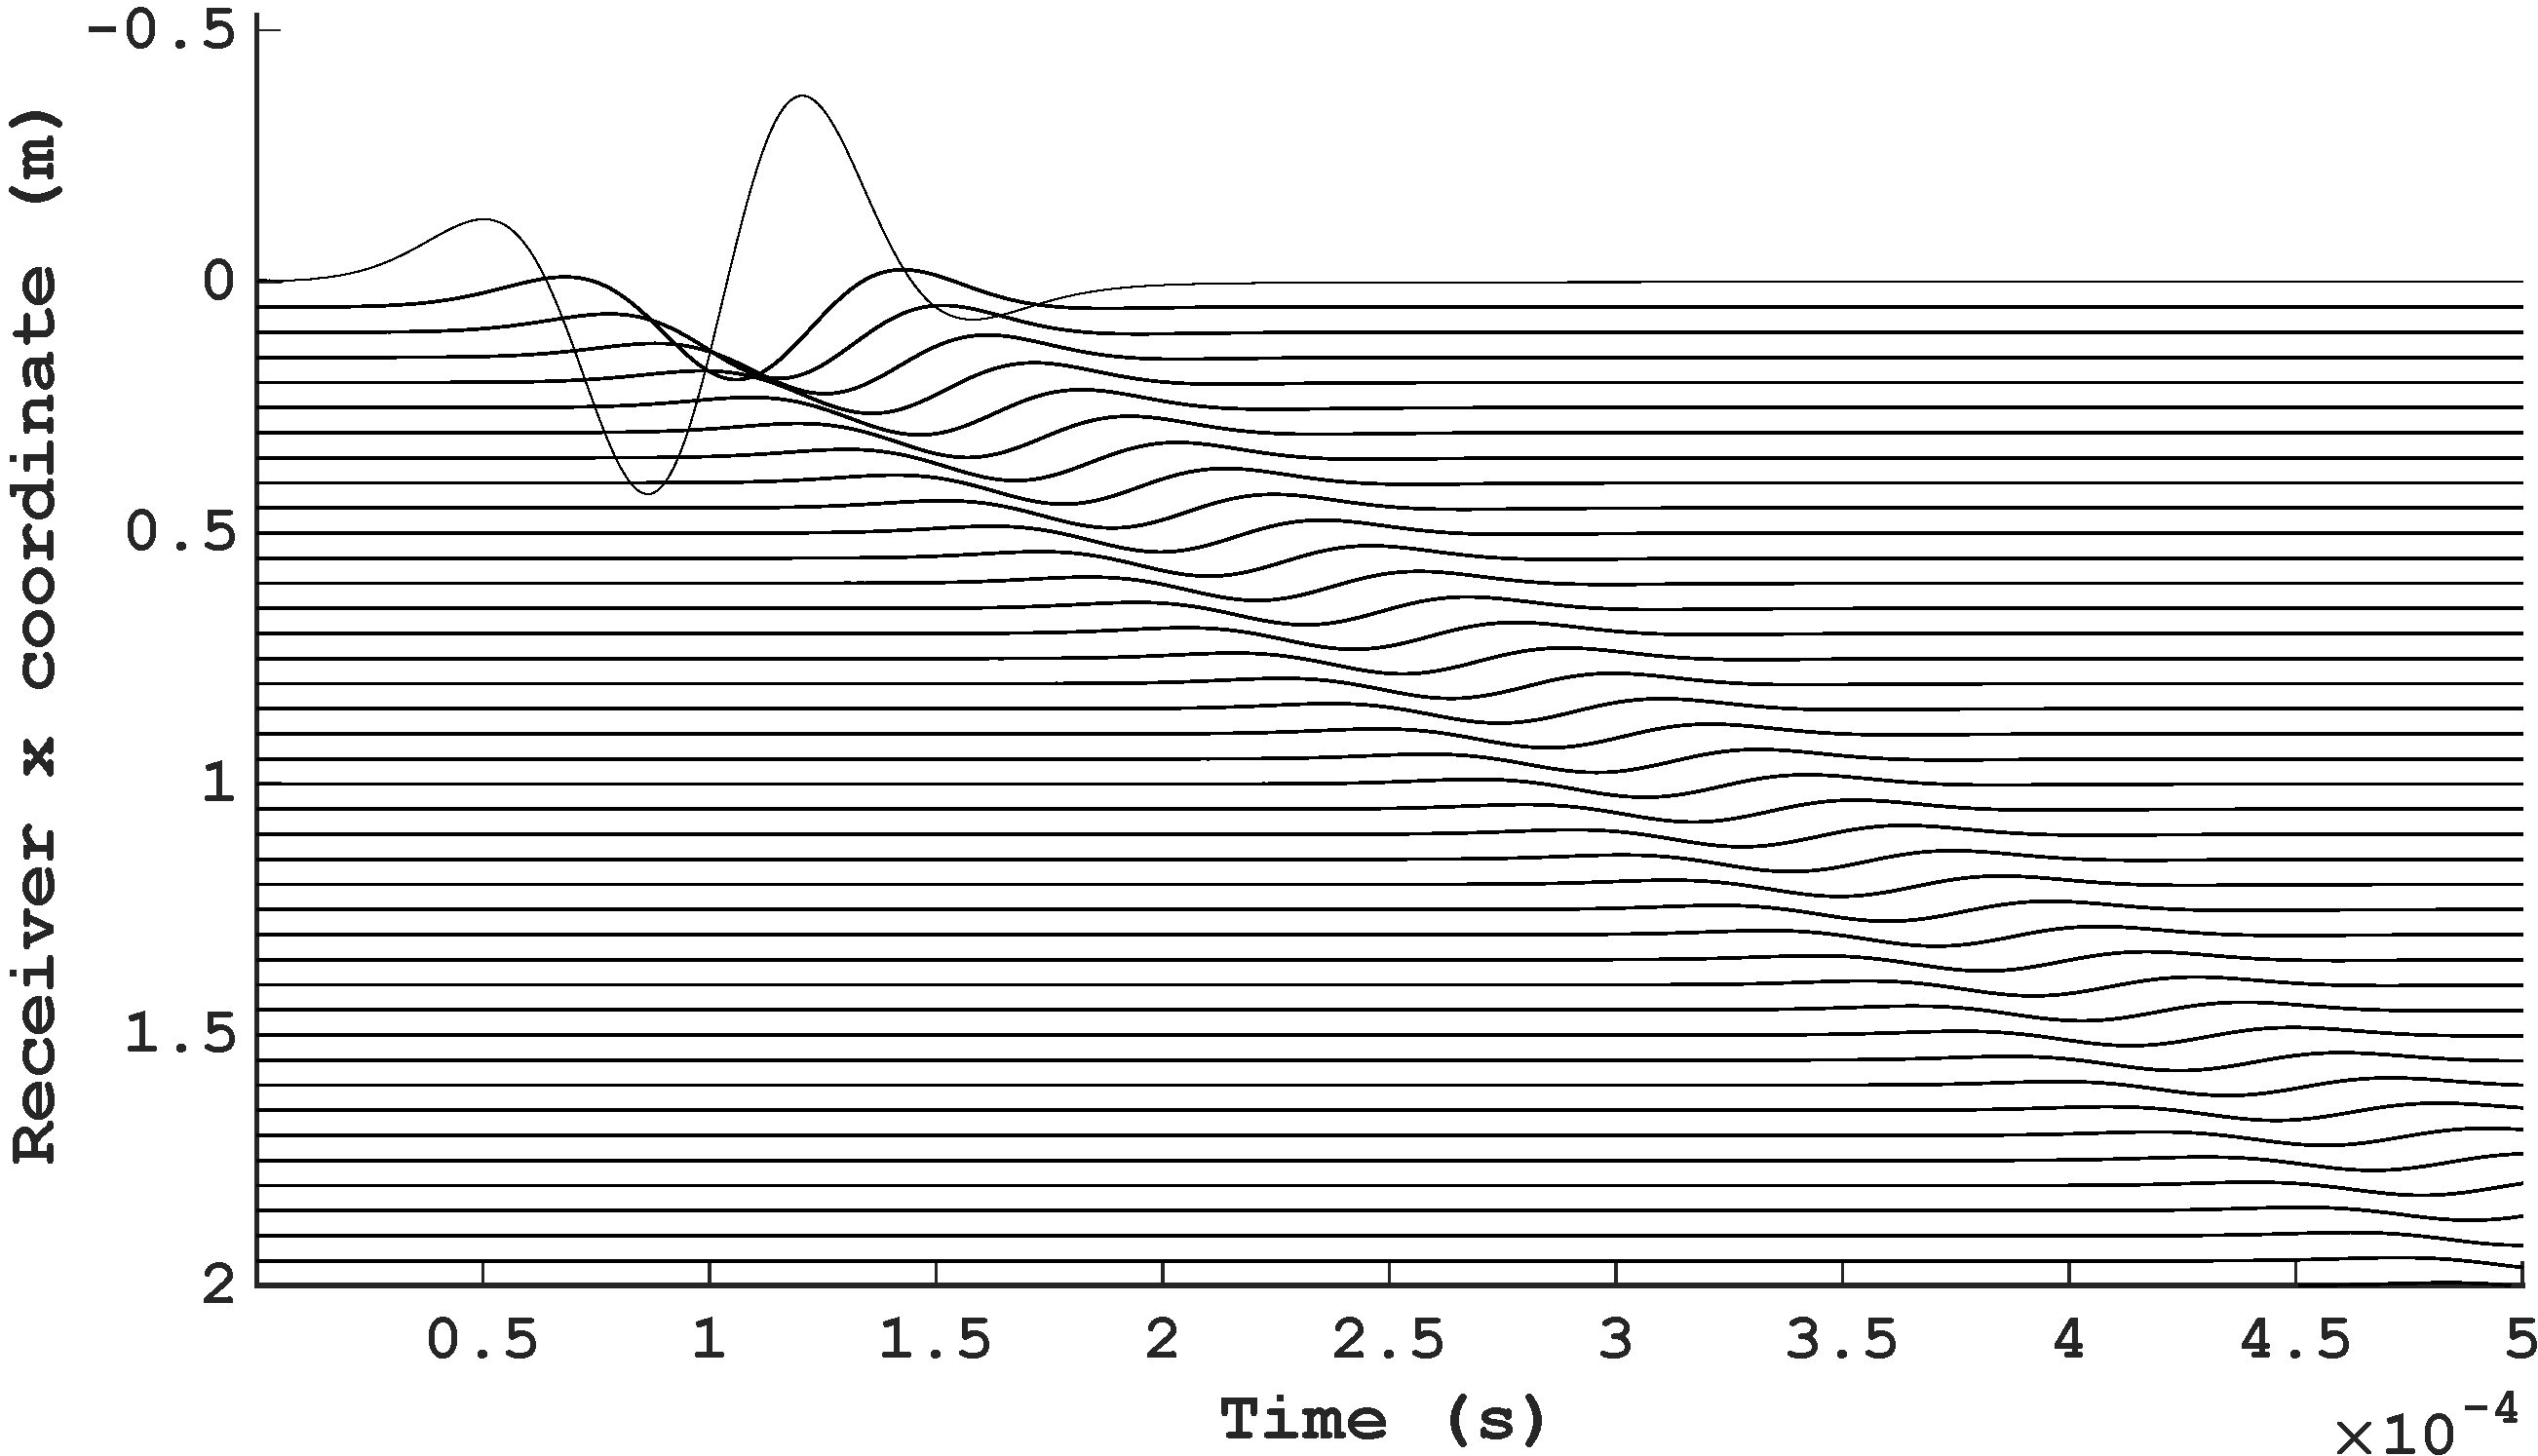
\includegraphics[draft=false,width=1\textwidth, 
height=0.15\textheight]{Figures/frec_10_4_new2}
\caption{$\quad\quad f_0=10^{4} $}
\end{subfigure}
\hfill
\begin{subfigure}{0.3\linewidth}
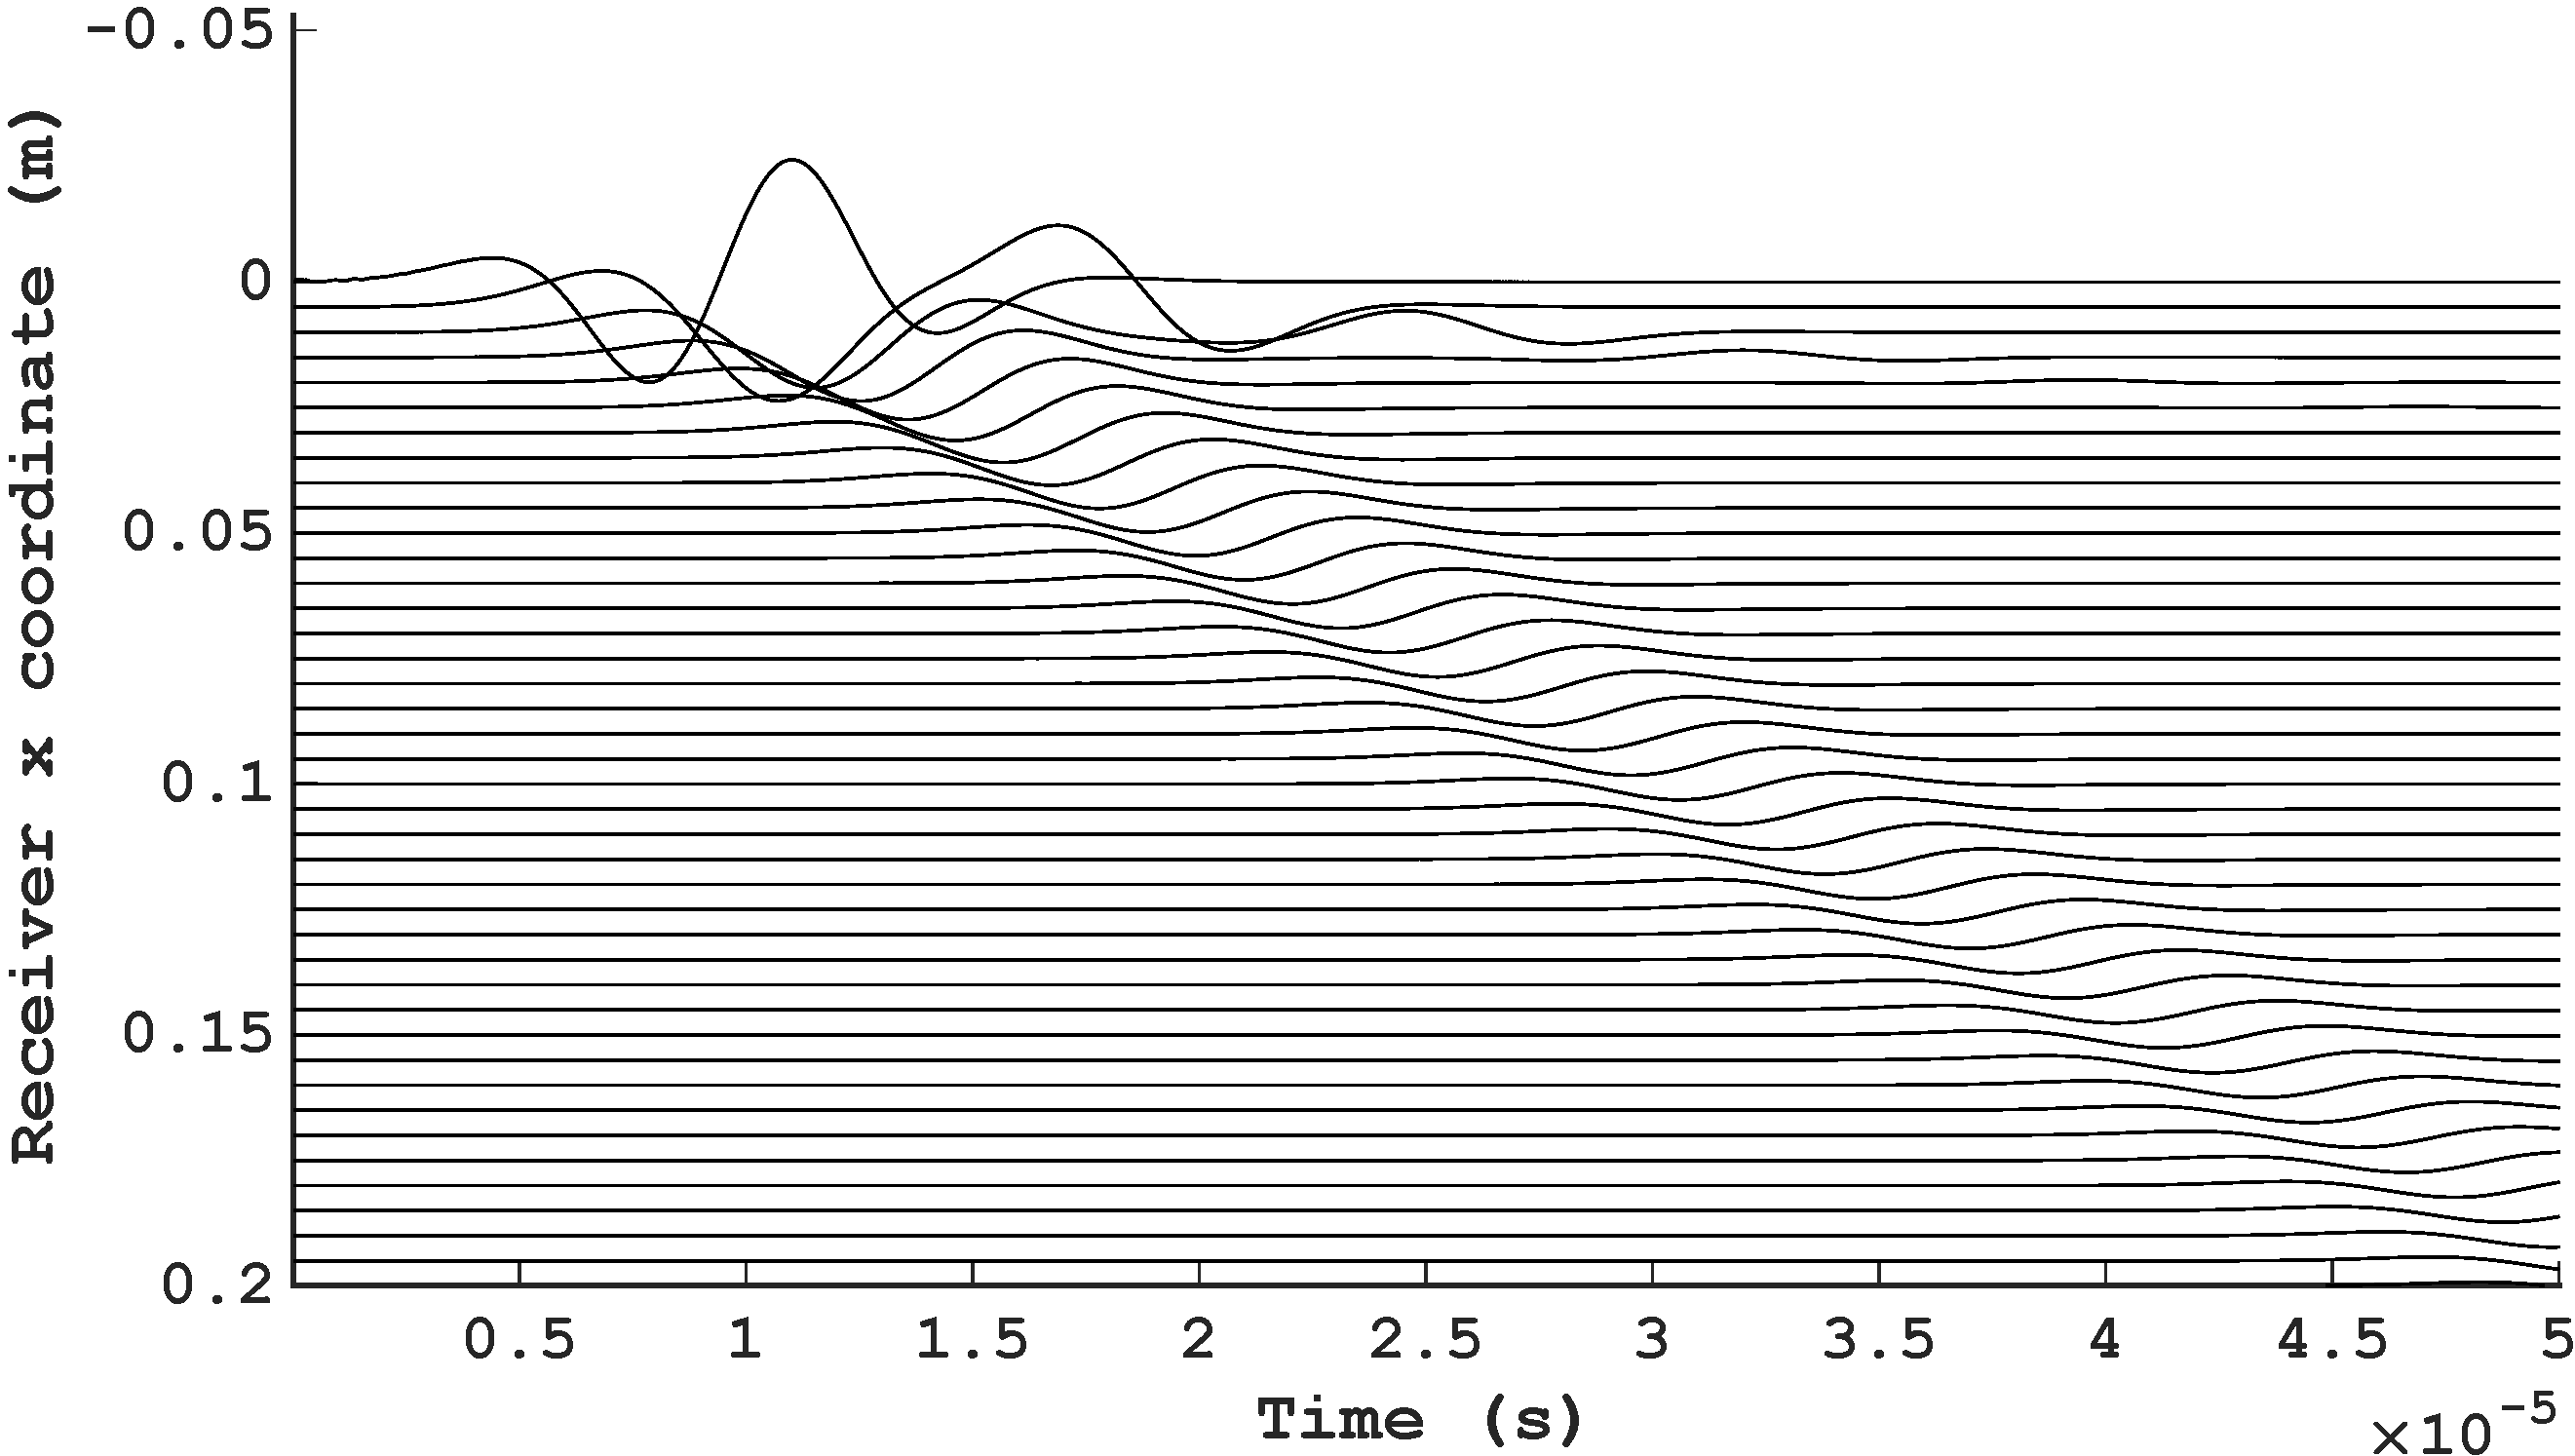
\includegraphics[draft=false,width=1\textwidth, 
height=0.15\textheight]{Figures/frec_10_5_new2}
\caption{$\quad\quad f_0=10^{5} $}
\end{subfigure}%
\hfill
\begin{subfigure}{0.3\linewidth}
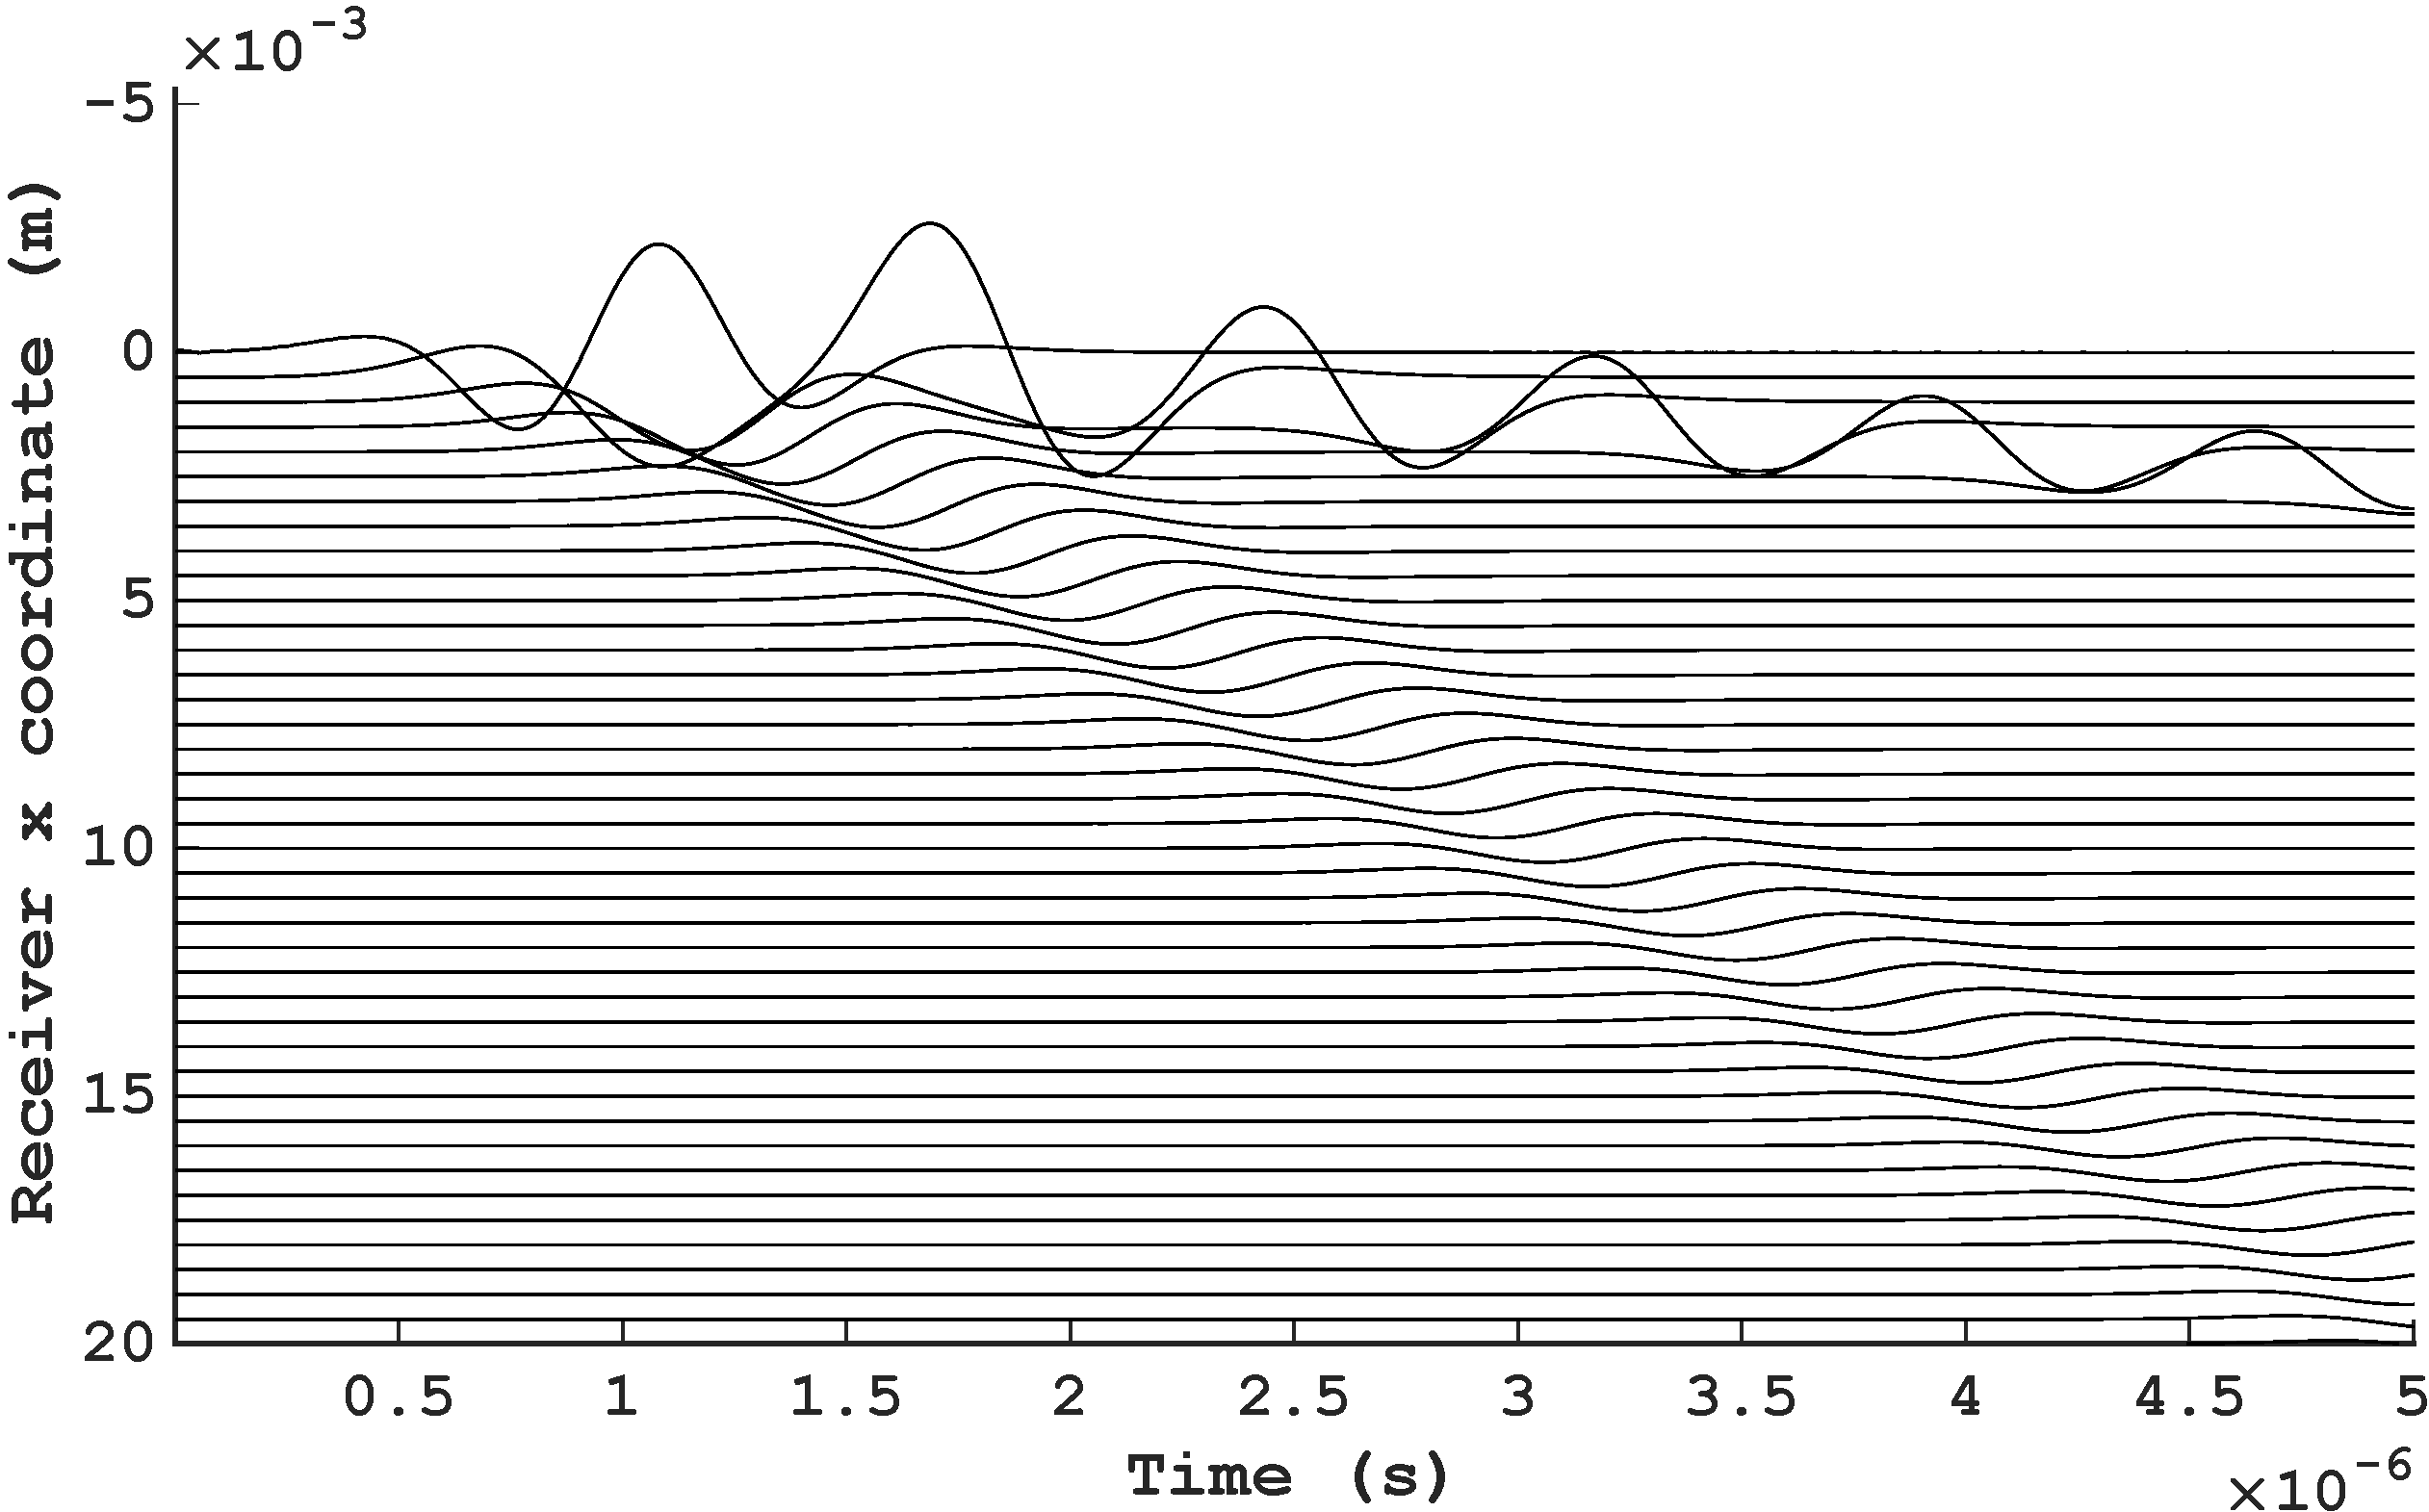
\includegraphics[draft=false,width=1\textwidth, 
height=0.15\textheight]{Figures/frec_10_6_new2}
\caption{$\quad\quad f_0=10^{6} $}
\end{subfigure}%
\caption{ A seismograms of the mixture velocity $v^1$ for different frequencies: $f_0=10^{4}$ Hz (a), $f_0=10^{5}$ Hz (b), $f_0=10^{6}$ Hz(c) .  }
\label{fig:compare_frewuency_trace}
\end{figure}

%PS Reference: (Gurevich and Pevzner 2015, Appendix B: in Caspari et al, 2019. %Reference: Gurevich B. and Pevzner R. 2015. How frequency dependency of Q affects %spectral ratio estimates. Geophysics 80, A39–A44.; Caspari E., Novikov M., Lisita V., %Barbosa N. D., Quintal B., Rubino J. G., Holliger K., 2019, Attenuation mechanisms in %fractured fluid-saturated porous rocks: a numerical modelling study, Geophysical %Prospecting, 67, 935–955, doi: 10.1111/1365-2478.12667).

\subsection{Dependence on the shear relaxation time.}


The aim of this section is to show that there is an additional mechanism of 
energy dissipation embedded in system \eqref{stress.velocity} and controlled 
by the relaxation parameter $\tau$ on the right-hand side of equation
\eqref{sij}. A proper choice of the relaxation time $ \tau $ allows one to 
model 
irreversible (elastoplastic) deformations in the solid matrix, e.g. 
\cite{HYP2016,Hyper-Hypo2019}, or viscous flows \cite{DPRZ2016}.

All the previous numerical examples were done without relaxation of tangential 
shear stresses, that is, the right-hand side in \eqref{sij} vanishes. Formally, 
this corresponds to the case of $\tau=\infty$. It is quite obvious that for 
finite values of
$ \tau $, the mechanism of tangential stresses relaxation provides 
another ability of the model to 
control the wave attenuation. To this end, we again 
consider an 
example from the previous Section\,\ref{sec.frequency} for the frequency 
$f_0=10^{4}$ Hz and compare 
the solution with a similar test but with allowance for the relaxation of 
tangential stresses.
\begin{figure}[!htbp]
	\begin{center}
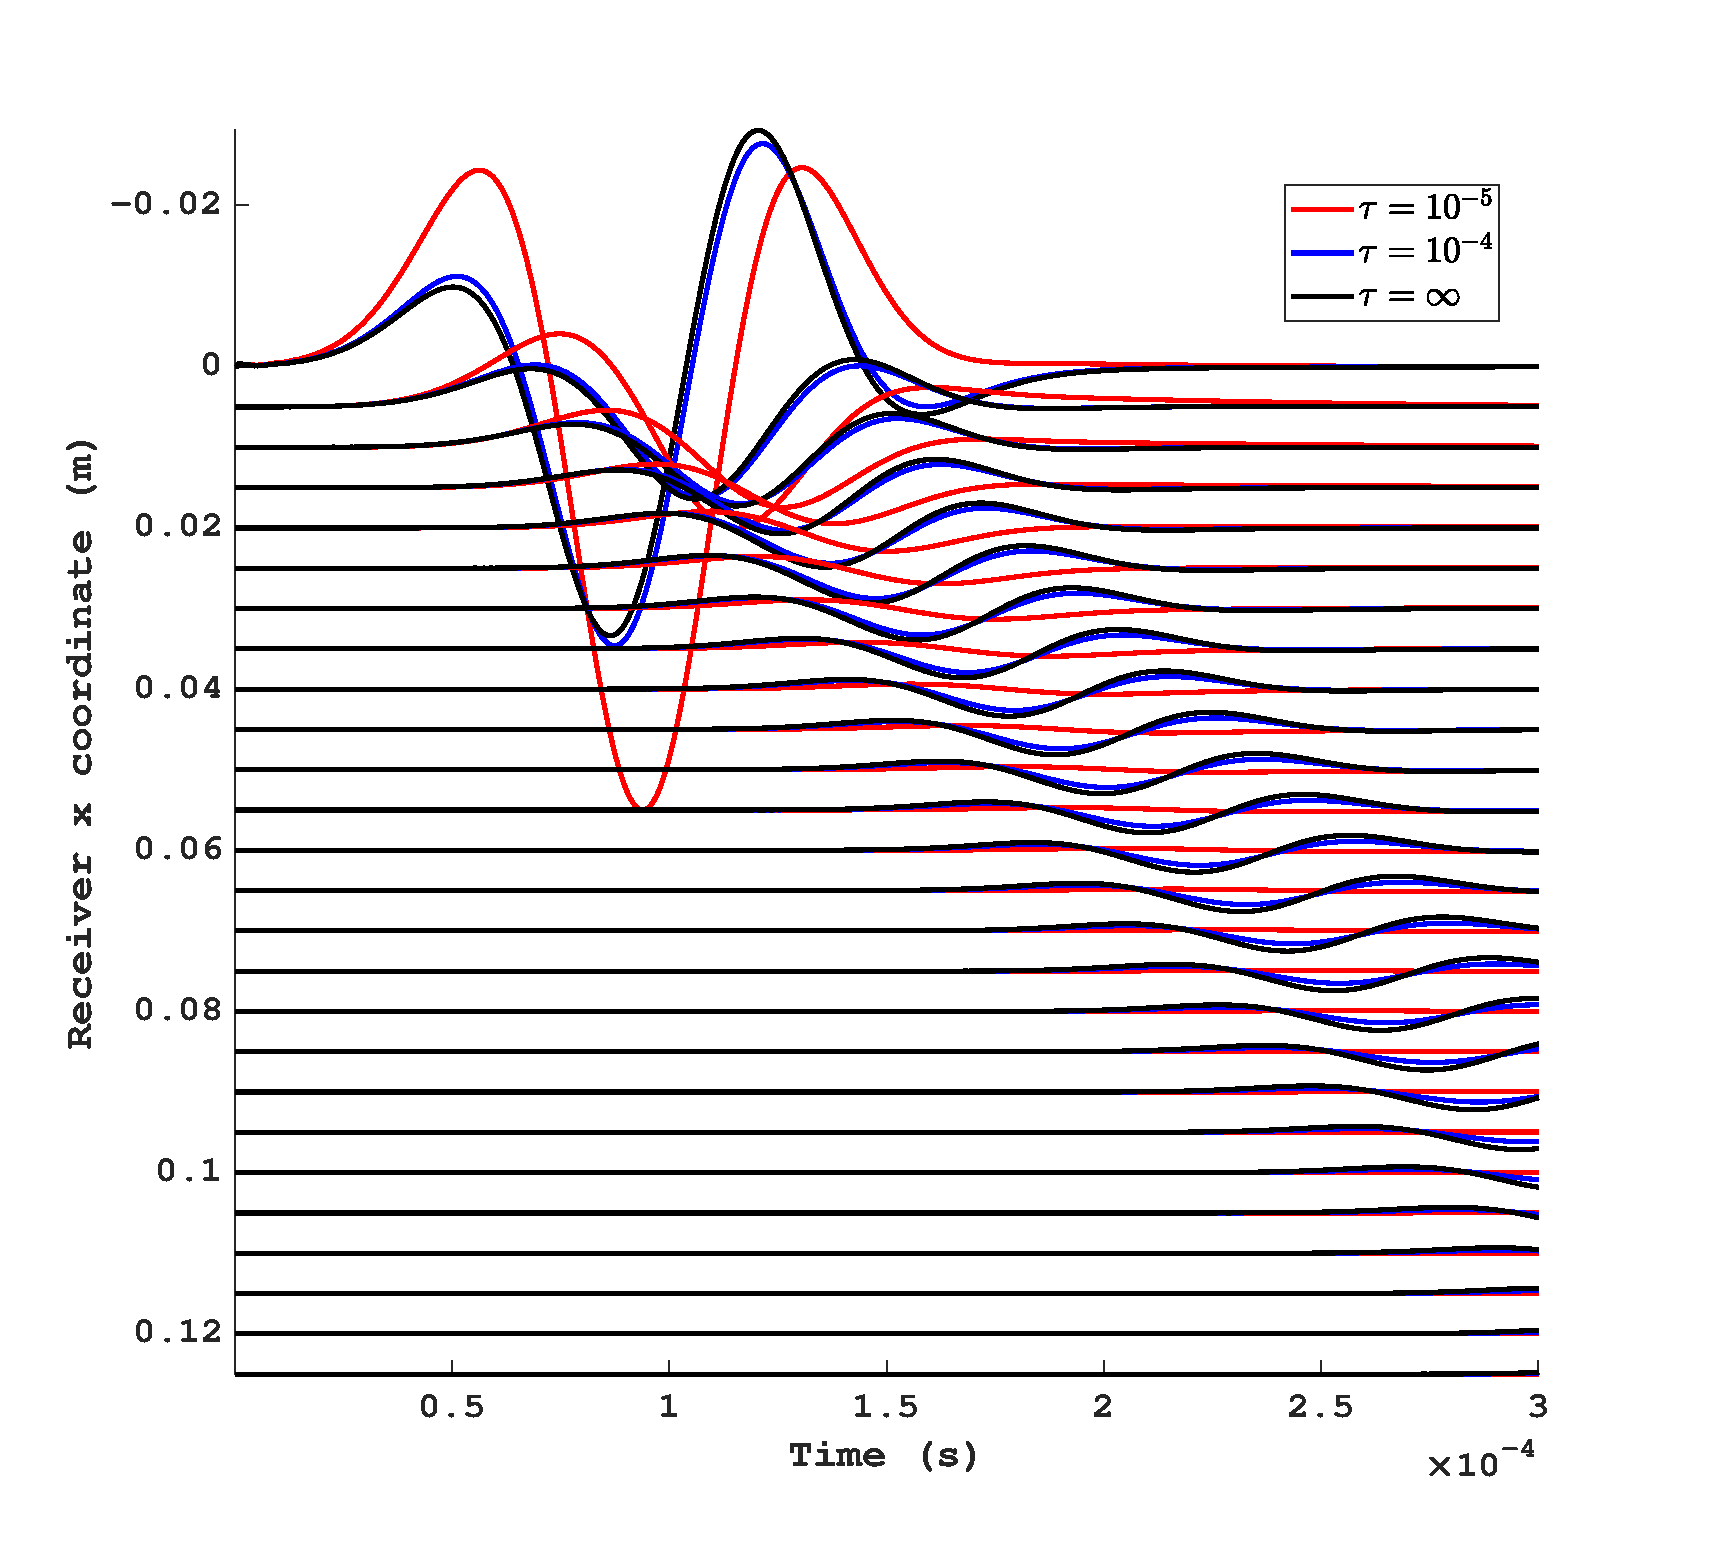
\includegraphics[draft=false,width=0.75\textwidth]{Figures/Compare_dissip_10_4}
	\end{center}
	\caption{{\footnotesize \it  
	Comparison of the seismograms of the mixture velocity $v^1$  for different 
	values of $\tau$:
	no dissipation - black, $\tau=10^{-5}$ - red, $\tau=10^{-4}$ - blue.}}
	\label{fig: Compare_dissip}
\end{figure}
As one would expect, a comparison of the seismograms in Fig.\,\ref{fig: Compare_dissip} shows that the relaxation of tangential stresses leads to the dispersion and attenuation of seismic waves. On the receivers that are far away, it is seen that the smaller $\tau$, the greater the attenuation. On the near receivers, the dispersion probably gives the predominant effect.


\subsection{Layered media.}

This test illustrates the interface effects between a pure fluid, poroelastic 
and 
pure elastic media on the example of a three-layered medium with the material 
parameters from Table 
\ref{tab:parameters}. The size of the computational domain is $0.025$\,m in the 
$ x $ and $ y $ directions. The upper layer is water, the lower layer is the
elastic 
medium and in the middle, from $-0.005$ m to $0.005$ m, there is a poroelastic 
layer with porosity $\phi$=0.2. The source of central frequency $f_0=10^{6}$ Hz 
is located in the water at the point $x=0, y=-0.01$. 

In order to present all types of waves let us consider snapshots  for the total 
velocity vector  for different moments of time. We strongly amplified the 
wavefield amplitude in Fig.\,\ref{fig: layered_snap} to be able to pick out the 
slow compressional waves on the snaps. In order to interpret the waves arising 
in the medium, we use capital 'P' to mark P-waves  and capital 'S' to 
mark S-waves. The subscript 'r'  indicates the reflected waves, while 
subscript 't'  indicates the transmitted waves. Also, we use the 
subscript 's' to identify a slow P-wave and subscript 'f' to identify the 
pressure wave in the fluid layer.

A source in the water excites a pressure wave (denoted as P$_\textrm{f}$ in 
Fig.\,\ref{fig: 
layered_snap}) which propagates towards the a poroelastic layer.
This wave then reflects from the bottom of the water-poroelastic interface 
(P$_\textrm f$P$_\textrm r$) and generates a fast transmitted P-wave 
(P$_\textrm f$P$_\textrm t$),  slow 
transmitted P-wave (P$_\textrm f$P$_\textrm s$) and transmitted 
S-wave (P$_\textrm f$S$_\textrm t$) in the  poroelastic medium. Afterwards, 
these waves generate the 
family of transmitted and reflect waves (including transmitted P-wave 
(P$_\textrm f$P$_\textrm t$P$_\textrm t$) and S-wave 
(P$_\textrm f$S$_\textrm t$S$_\textrm t$) and 
reflected slow P-wave (P$_\textrm f$P$_\textrm t$P$_\textrm s$)) from the  
upper and lower boundaries of 
the poroelastic layer. 

In this example, we see the correct propagation of all types of waves, 
predicted by elasticity and poroelasticity theories: the slow waves arise only 
in poroelastic layer, only pressure wave propagate in a liquid, while the  
longitudinal and shear waves appear in the elastic medium.
\begin{figure}[!htbp]
	\begin{center}
	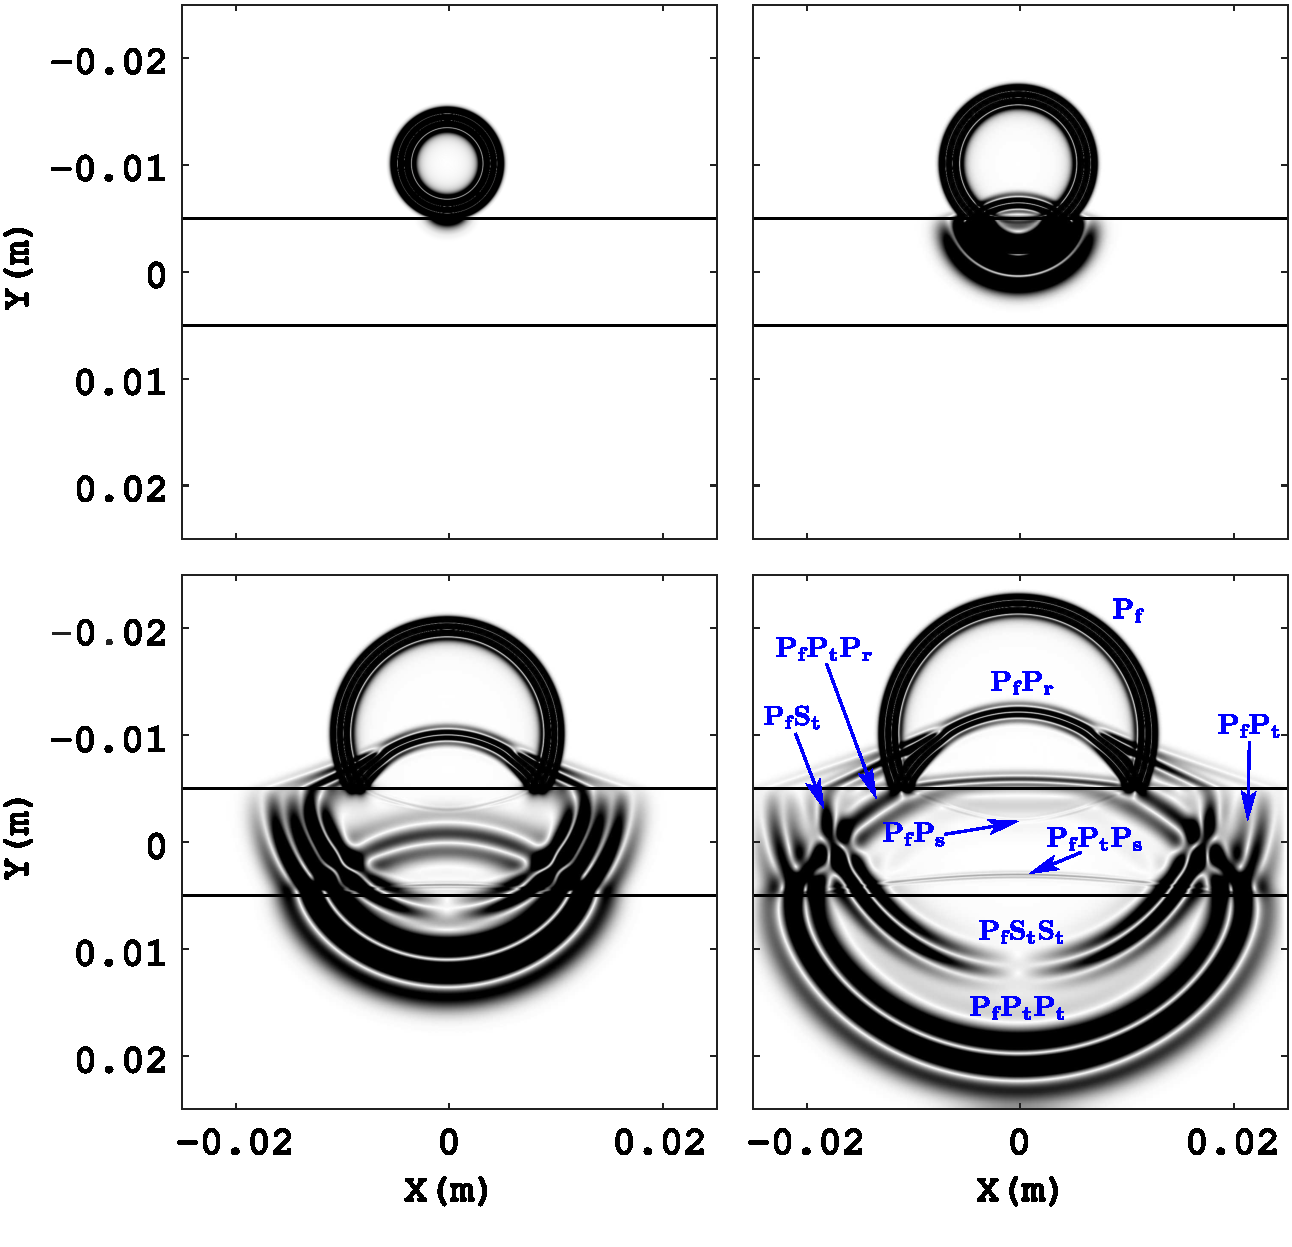
\includegraphics[draft=false,width=0.8\textwidth]{Figures/Layered_media_u1_u2_v4}
	\end{center}
	\caption{{\footnotesize \it  Snapshots of $ ||v||^2 $ for the layered medium: water (upper 
	layer, $ \phi=1 $), poroelastic (middle layer,  $ \phi=0.2 $) and elastic 
	solid  (bottom layer, $ \phi=0 $).}}
	\label{fig: layered_snap}
\end{figure}


\section{Conclusions}

An extension of the unified model of continuum fluid and solid mechanics 
\cite{DPRZ2016} for compressible fluid flows in elastoplastic porous media has 
been proposed.
The derivation  is based on the Symmetric Hyperbolic 
Thermodynamically Compatible (SHTC) theory \cite{SHTC-GENERIC-CMAT} and the 
resulting model represents the coupling of the unified continuum model from 
\cite{DPRZ2016} with the SHTC model for two-phase compressible flows from 
\cite{RomDrikToro2010}.
The governing equations satisfy the two laws of thermodynamics (energy 
conservation and non-decreasing of the entropy) and form first-order symmetric  
system, 
which 
is hyperbolic in the sense of Friedrichs \cite{Friedrichs1958}, if the 
generating thermodynamic potential is convex.

Based on the proposed non-linear model, the lineraised first order PDE system 
for small amplitude wave propagation in a stationary saturated porous medium 
has been derived. The linear system is written in terms of the velocity of the 
solid-fluid mixture, relative velocity of the phase motion, pressure and shear 
stress. Such a formulation allowed us a straightforward development of the 
efficient finite-difference scheme on staggered grid.  

The comparison of the proposed SHTC model and classical Biot's model for wave 
propagation in the saturated elastic porous  medium has been done.
It turns out that although the basic equations of the two models are different, 
the SHTC model is able to describe all the effects (in particular, the 
existence of slow P-wave) predicted by Biot's theory, with good quantitative 
and qualitative agreement.

A series of test problems solved for SHTC model for different values of 
parameters of the model, including porosity and interfacial friction, has been 
solved. The numerical results demonstrate that the SHTC model describes 
correctly all physical characteristics of the process.   

\section*{Acknowledgements}
% 
The research of E.R. and G.R. in Sects.2-4 was supported by the Russian Science Foundation  under grant 19-77-20004, the research in Sect.5 was supported by the Russian Foundation for Basic Research under grant 19-01-00347.
I.P. gratefully acknowledges the support of Agence Nationale de la Recherche (FR) 
(grant ANR-11-LABX-0040-CIMI) under program ANR-11-IDEX-0002-02.
The work of M.D. was partially supported by the European Union's Horizon 2020 Research and Innovation  Programme under project \textit{ExaHyPE}. 
MD also gratefully acknowledges funding from the Italian Ministry of Education, University and Research (MIUR) under the Departments of Excellence Initiative 2018--2022 attributed to DICAM of the University of Trento, as well as financial support from the University of Trento under the  \textit{Strategic Initiative Modeling and Simulation}.



\printbibliography






\end{document}
%	
%	\bibitem{Ishii1975}
%	Ishii M. \emph{Thermo-fluid dynamic theory of two-phase flow}. Eyrolles, Paris, 1975.
%	
%	\bibitem{Stewart1984} 
%	Stewart BH, Wendroff B. Two-phase flow: models and methods. \emph{J. Comp. Phys.} 1984; 
%\textbf{56}:363.
%	
%	\bibitem{Staedke2005}
%	Staedke H, Francello G, et al. Advanced three-dimensional flow simulation tools for application 
%to reactor safety (ASTAR).
%	\emph{Nuclear Engineering and Design} 2005; \textbf{235}:379.
%	
%	\bibitem{Baer1986}
%	Baer M, Nunziato J. A two-phase mixture theory for the deflagration-to-detonation transition 
%(DDT) in reactive granular materials.
%	\emph{Int. J. Multiphase Flow} 1986; \textbf{12}:861.
%	
%	\bibitem{Saurel1999}
%	Saurel R, Abgrall R. A multiphase Godunov method for compressible multi-fluid and multiphase 
%flows.
%	\emph{J. Comput. Phys.} 1999; \textbf{150}:425.
%	
%	\bibitem{LeMetayer2005}
%	Le~Metayer O, Massoni J, Saurel R. Modelling evaporation fronts with reactive Riemann solvers. 
%\emph{J. Comput. Phys.} 2005; \textbf{205}:567.https://www.overleaf.com/5968336422cdvbzvsbmgxd
%	
%	\bibitem{Kreeft&Koren2010}
%	Kreeft JJ, Koren B. A new formulation of Kapila's
%	five-equation model for compressible two-fluid flow, and its
%	numerical treatment, {\it J. Comput. Phys.} 2010, \textbf{229}:6220.
%	
%	\bibitem{Zein2010}
%	Zein A, Hantke M, Warnecke G. Modeling phase transition for
%	compressible two-phase flows applied to metastable liquids,
%	\emph{J. Comput. Phys.} 2010; \textbf{229}:2964.
%	
%	\bibitem{Herard2007}
%	Herard JM. A Three-Phase Flow Model. \emph{Math. Comput.
%		Modelling} 2007; \textbf{45}:732.
%	
%	\bibitem{Abgrall}
%	
%	Abgrall R, Saurel R. Discrete equations for physical and numerical compressible
%	multiphase mixtures. {\it J. Comput. Phys.} 2003, \textbf{186}:361.
%	
%	\bibitem{Romenski2001}
%	Romensky E. Thermodynamics and hyperbolic systems of balance
%	laws in continuum mechanics. In \emph{Godunov Methods: theory
%		and applications}, Toro EF. (ed). Kluwer Academic/Plenum
%	Publishers, NY, 2001.
%	
%	\bibitem{Godunov2003}
%	Godunov SK, Romenski E. \emph{Elements of continuum mechanics and conservation laws}, Kluwer 
%Academic/Plenum Publishers, NY, 2003.
%	
%	\bibitem{Muller1998}
%	Muller I, Ruggeri T. \emph{Rational extended thermodynamics}, Springer-Verlag, NY, 1998.
%	
%	
%	\bibitem{Romenski2004}
%	Romenski E, Toro EF. Compressible two-phase flows: two-pressure models and numerical methods. 
%\emph{Computational Fluid Dynamics J.} 2004; \textbf{13}:403.
%	
%	\bibitem{Romenski2007}
%	Romenski E, Resnyansky AD, Toro EF. Conservative hyperbolic model for compressible two-phase 
%flow with different phase pressures and temperatures. \emph{Quarterly Applied Math.} 2007; 
%\textbf{65}:259.
%	
%	\bibitem{RomDrikToro2010}
%	Romenski E, Drikakis D, Toro EF. Conservative models and numerical methods for one-dimensional 
%compressible two-phase flow. \emph{J. Sci. Comp.} 2010; \textbf{42}:68.
%	
%	\bibitem{Mattia}
%	La~Spina G, De'Michieli~Vitturi M. High resolution finite volume central schemes for a 
%compressibile two-phase model, \emph{SIAM J. Sci. Comp.} 2012; \textbf{34}: B861. 
%	
%	\bibitem{Romenski2012_It}
%	De'Michieli~Vitturi M, La~Spina G, Romenski E. 
%	A compressible single temperature conservative two-phase model with phase
%	transitions. in \emph{Numerical Analysis and
%		Applied Mathematics ICNAAM 2013}, Simos TE, Psihoyios G, Tsitouras Ch (eds),
%	AIP Conf. Proc.; \textbf{1558}:112, American Institute of Physics, NY, 2013.
%	
%	
%	\bibitem{Zeidan2011}
%	Zeidan D. On a further work of two-phase mixture conservation laws.
%	in \emph{Numerical Analysis and Applied Mathematics ICNAAM 2011}, Simos TE, Psihoyios G, 
%Tsitouras Ch, Zacharias Anastassi (eds),  AIP Conf. Proc.; \textbf{1389}:163, American Institute 
%of 
%Physics, NY,   2011.
%	
%	
%	\bibitem{Romenski2012}
%	Romenski E. Hyperbolic systems of conservation laws for
%	compressible multiphase flows based on thermodynamically
%	compatible systems theory, in \emph{Numerical Analysis and
%		Applied Mathematics ICNAAM 2012}, Simos TE, Psihoyios G, Tsitouras Ch, Zacharias Anastassi 
%(eds), AIP Conf. Proc. \textbf{1479}:62, American Institute of Physics, NY, 2012.
%	
%	\bibitem{ToroBook}
%	{Toro EF.}  \textit{Riemann solvers and numerical methods in
%		fluid dynamics} Springer-Verlag, Second Edition,1999.
%	
%	\bibitem{friedrichs1954}
%	{Friedrichs KO.} {Symmetric hyperbolic linear differential
%		equations}. \textit{Comm. Pure Appl. Math.} 1954; {\bf 7}: 
%	345.
%	
%	\bibitem{ToroTitarev}
%	{Toro EF, Titarev VA.}  {MUSTA schemes for systems of
%		conservation laws}, {\it J. Comput. Phys.}2006 \textbf{216}: 403.
%	
